%% 
%% Copyright 2007-2020 Elsevier Ltd
%% 
%% This file is part of the 'Elsarticle Bundle'.
%% ---------------------------------------------
%% 
%% It may be distributed under the conditions of the LaTeX Project Public
%% License, either version 1.2 of this license or (at your option) any
%% later version.  The latest version of this license is in
%%    http://www.latex-project.org/lppl.txt
%% and version 1.2 or later is part of all distributions of LaTeX
%% version 1999/12/01 or later.
%% 
%% The list of all files belonging to the 'Elsarticle Bundle' is
%% given in the file `manifest.txt'.
%% 

%% Template article for Elsevier's document class `elsarticle'
%% with numbered style bibliographic references
%% SP 2008/03/01
%%
%% 
%%
%% $Id: elsarticle-template-num.tex 190 2020-11-23 11:12:32Z rishi $
%%
%%
\documentclass[preprint,12pt]{elsarticle}

%% Use the option review to obtain double line spacing
%% \documentclass[authoryear,preprint,review,12pt]{elsarticle}

%% Use the options 1p,twocolumn; 3p; 3p,twocolumn; 5p; or 5p,twocolumn
%% for a journal layout:
%% \documentclass[final,1p,times]{elsarticle}
%% \documentclass[final,1p,times,twocolumn]{elsarticle}
%% \documentclass[final,3p,times]{elsarticle}
%% \documentclass[final,3p,times,twocolumn]{elsarticle}
%% \documentclass[final,5p,times]{elsarticle}
%% \documentclass[final,5p,times,twocolumn]{elsarticle}

%% For including figures, graphicx.sty has been loaded in
%% elsarticle.cls. If you prefer to use the old commands
%% please give \usepackage{epsfig}

%% The amssymb package provides various useful mathematical symbols
\usepackage{amssymb}
\usepackage{amsmath}
\usepackage{graphicx}
\usepackage{float}
%%\usepackage{wrapfig}
\usepackage{lscape}
\usepackage{rotating}
%%\usepackage{epstopdf}
\usepackage[font={small,it}]{caption}
\usepackage{subcaption}
\graphicspath{{figures/}}
\usepackage{lineno}
\linenumbers

%% The amsthm package provides extended theorem environments
%% \usepackage{amsthm}

%% The lineno packages adds line numbers. Start line numbering with
%% \begin{linenumbers}, end it with \end {linenumbers}. Or switch it on
%% for the whole article with \linenumbers.
%% \usepackage{lineno}

\journal{Arxiv}

\begin{document}
%.......................................................................
%  Define some latex commands to reduce the length of the equations
%......................................................................
\newcommand{\pd}[2]{\ensuremath{\frac{\partial#1}{\partial#2}}  }
\newcommand{\pbox}[1]{\ensuremath{\parbox[b]{.27\linewidth}{ \scriptsize \textsf {#1}}}  }
\newcommand{\pboxsmall}[1]{\ensuremath{\parbox[c]{.2\linewidth}{\scriptsize{#1}}}  }
\newcommand{\graybox}[1]{\psboxit{box .7 setgray fill}{\fbox{#1}} }
\newcommand{\half}          {\ensuremath{\tiny{\frac{1}{2}}}}
%
%.......................................................................
%  SINGLE MATEERIAL
%......................................................................
%..............................
%  no time superscript
%..............................                
\newcommand{\U}             {{\vec{U}}}                    
\newcommand{\uo}            {\ensuremath{\vec{U}_o}}                  
\newcommand{\delt}          {\ensuremath{\Delta{t}} }                 
\newcommand{\delx}          {\ensuremath{\Delta{x}} }                 
\newcommand{\dely}          {\ensuremath{\Delta{y}} }                 
\newcommand{\delz}          {\ensuremath{\Delta{z}} }
\newcommand{\delV}          {\ensuremath{\Delta{V}} }                 
\newcommand{\rhoo}          {\ensuremath{\rho_o}}
\newcommand{\rr}            {\ensuremath{\mathbf{r}}   }                     
\newcommand{\sumarea}       {\ensuremath{\sum_{i=1}^{n}}} 
\newcommand{\XCC}           {\ensuremath{\frac{\delx}{2}}}
\newcommand{\YCC}           {\ensuremath{\frac{\dely}{2}}}
\newcommand{\ZCC}           {\ensuremath{\frac{\delz}{2}}}
\newcommand{\angler}        {\ensuremath{\langle\mathbf{r}\rangle}   }        
%
%..............................
%  time n quantities
%..............................
\newcommand{\un}            {\ensuremath{\vec{U}^{n}}}
\newcommand{\unc}           {\ensuremath{\vec{U}^{n^{c}}}}               
\newcommand{\Tnc}           {\ensuremath{T^{n^{c}}}}                     
\newcommand{\pnc}           {\ensuremath{p^{n^c}} }                      
\newcommand{\en}            {\ensuremath{e^{n}}}                         
\newcommand{\mnc}           {\ensuremath{m^{n^{c}}}}                     
\newcommand{\Vnf}           {\ensuremath{V^{n^{f}}}} 
\newcommand{\Vn}            {\ensuremath{V^{n}} }                    
\newcommand{\mnf}           {\ensuremath{m^{n^{f}}}}                
\newcommand{\unf}           {\ensuremath{\vec{U}^{n^{f}}}}          
\newcommand{\rhonf}         {\ensuremath{\rho^{n^{f}}}}             
\newcommand{\rhonc}         {\ensuremath{\rho^{n^{c}}}}             
\newcommand{\rhoncl}        {\ensuremath{\rho^{n^{c}}_r}}           
\newcommand{\spvol}         {\ensuremath{ \upsilon^{n^{c}} } }
\newcommand{\uvelnc}        {\ensuremath{ u^{n^{c}} } }
\newcommand{\vvelnc}        {\ensuremath{ v^{n^{c}} } }
\newcommand{\wvelnc}        {\ensuremath{ w^{n^{c}} } }
\newcommand{\momnc}         {\ensuremath{(m\vec{U})^{n^{c}} } }
\newcommand{\engnc}         {\ensuremath{E^{n^{c}} } }
%..............................
%  n quantities I,J,K
%..............................
\newcommand{\unIJK}         {\ensuremath{u^{n}_{i,j,k}}}
\newcommand{\TnIJK}         {\ensuremath{T^{n}_{i,j,k}}}
\newcommand{\cvIJK}         {\ensuremath{c_{v_{i,j,k}}}}
\newcommand{\uncIJK}        {\ensuremath{u^{n^{c}}_{i,j,k}}}
\newcommand{\vnIJK}         {\ensuremath{v^{n}_{i,j,k}}}
\newcommand{\VnIJK}         {\ensuremath{V^{n}_{i,j,k}}}
\newcommand{\vncIJK}        {\ensuremath{v^{n^{c}}_{i,j,k}}}
\newcommand{\wnIJK}         {\ensuremath{w^{n}_{i,j,k}}}
\newcommand{\wncIJK}        {\ensuremath{w^{n^{c}}_{i,j,k}}}
\newcommand{\uijkl}         {\ensuremath{ u^{*^{f}}_{{i,j,k,L}}}}
\newcommand{\uijkr}         {\ensuremath{ u^{*^{f}}_{{i,j,k,R}}}}
\newcommand{\vijkt}         {\ensuremath{ v^{*^{f}}_{{i,j,k,T}}}}
\newcommand{\vijkb}         {\ensuremath{ v^{*^{f}}_{{i,j,k,B}}}}
\newcommand{\wijkf}         {\ensuremath{ w^{*^{f}}_{{i,j,k,FR}}}}
\newcommand{\wijkbk}        {\ensuremath{ w^{*^{f}}_{{i,j,k,BK}}}}
\newcommand{\rhonIJK}       {\ensuremath{\rho^{n}_{i,j,k}}}
%
%..............................
%  n + 1 quantities
%..............................
\newcommand{\nadv}          {\text{\tiny{n+1}}}                             
\newcommand{\unnL}          {\ensuremath{\vec{U}^{\nadv^{L}}}}              
\newcommand{\unnf}          {\ensuremath{\vec{U}^{\nadv^{{f}}}}}          
\newcommand{\unnc}          {\ensuremath{\vec{U}^{\nadv^{c}}}}      
\newcommand{\VnnL}          {\ensuremath{V^{\nadv^{L}}}}
\newcommand{\uvelstar}      {\ensuremath{ u^{\nadv^{*^{f}}}}  }             
\newcommand{\vvelstar}      {\ensuremath{ v^{\nadv^{*^{f}}}}  }             
\newcommand{\wvelstar}      {\ensuremath{ w^{\nadv^{*^{f}}}}  }             
\newcommand{\TnnL}          {\ensuremath{ T^{\nadv^{L}}}  }
\newcommand{\Tnnc}          {\ensuremath{ T^{\nadv^{c}}}  }
\newcommand{\ustar}         {\ensuremath{\vec{U}^{\nadv^{*^{f}}}}}          
\newcommand{\udummy}        {\ensuremath{\hat{ \vec{U} }^{\nadv^{f}}  } }   
\newcommand{\pstar}         {\ensuremath{p^{\nadv^{*^{f}}}}}                
\newcommand{\pnnLc}         {\ensuremath{p^{\nadv^{L^c}}} }                 
\newcommand{\rhonnc}        {\ensuremath{\rho^{\nadv{^{c}}}}}
\newcommand{\rhonnL}        {\ensuremath{\rho^{\nadv{^{L}}}}} 
\newcommand{\rhonnf}        {\ensuremath{\rho^{\nadv{^{f}}}}}          
\newcommand{\delpc}         {\ensuremath{ \Delta p^{\nadv^{c}}  } }         
\newcommand{\momnnL}        {\ensuremath{(m\vec{U})^{\nadv^{L}} } }
\newcommand{\momnnc}        {\ensuremath{(m\vec{U})^{\nadv^{c}} } }
\newcommand{\massnnc}       {\ensuremath{m^{\nadv^{c}} } }
\newcommand{\massnnL}       {\ensuremath{m^{\nadv^{L}} } }
\newcommand{\massnnLf}      {\ensuremath{m^{\nadv^{L}^{f}} } }
\newcommand{\engnnc}        {\ensuremath{E^{\nadv^{c}} } }
\newcommand{\engnnL}        {\ensuremath{e^{\nadv^{L}} } }
\newcommand{\volfracnn}     {\ensuremath{\theta^{\nadv} } }
\newcommand{\delmomnn}      {\ensuremath{\Delta(m\vec{U})^{\nadv} } }  
\newcommand{\delengnn}      {\ensuremath{\Delta(mT)^{\nadv} } } 
\newcommand{\delmassnn}     {\ensuremath{\Delta(m)^{\nadv} } }
%          
%..............................
%  n + 1 quantities, i,j 
%..............................
\newcommand{\VnnLIJK}       {\ensuremath{V^{\nadv^{L}}_{i,j,k}}}
\newcommand{\unnLIJK}       {\ensuremath{u^{\nadv^{L}}_{i,j,k}}}
\newcommand{\vnnLIJK}       {\ensuremath{v^{\nadv^{L}}_{i,j,k}}}
\newcommand{\wnnLIJK}       {\ensuremath{w^{\nadv^{L}}_{i,j,k}}}
\newcommand{\rhonnLIJK}     {\ensuremath{\rho^{\nadv^{L}}_{i,j,k}}}
\newcommand{\massnnLIJK}     {\ensuremath{m^{\nadv^{L}}_{i,j,k}}}
\newcommand{\ennLIJK}     {\ensuremath{e^{\nadv^{L}}_{i,j,k}}}

\newcommand{\unnFIJK}       {\ensuremath{u^{\nadv^{*^{f}}}_{i,j,k}}}
\newcommand{\vnnFIJK}       {\ensuremath{v^{\nadv^{*^{f}}}_{i,j,k}}}
\newcommand{\wnnFIJK}       {\ensuremath{w^{\nadv^{*^{f}}}_{i,j,k}}}

%
%......................................................................
%  MULTIMATEERIAL
%......................................................................
\newcommand{\um}            {\ensuremath{\vec{U}_{m}}}                  
\newcommand{\rhom}          {\ensuremath{\rho_m}}                       
%
%..............................
%  n quantities
%..............................
\newcommand{\Vnm}           {\ensuremath{V^{n}_{m}}}                    
\newcommand{\massnm}        {\ensuremath{m^{n}_{m}}}                    
\newcommand{\unm}           {\ensuremath{\vec{U}^{n}_{m}}}
\newcommand{\unLm}          {\ensuremath{\vec{U}^{n^{L}}_{m}}}              
\newcommand{\Tnm}           {\ensuremath{T^{n}_{m}}}
\newcommand{\TnLm}          {\ensuremath{T^{n^{L}}_{m}}}                    
\newcommand{\engnm}         {\ensuremath{e^{n}_{m}}} 
\newcommand{\rhonm}         {\ensuremath{\rho^{n}_{m}}}
\newcommand{\momnm}         {\ensuremath{(m\vec{U})^{n}_{m} } }
%                   
%..............................
%  n+1 quantities 
%..............................
\newcommand{\unnm}          {\ensuremath{ \vec{U}^{\nadv}_{m}}  }
\newcommand{\unnLm}         {\ensuremath{\vec{U}^{\nadv^{L}}_{m}}}
\newcommand{\Tnnm}          {\ensuremath{ T^{\nadv}_{m}}  }
\newcommand{\TnnLm}         {\ensuremath{T^{\nadv^{L}}_{m}}}
\newcommand{\alpham}        {\ensuremath{\alpha_m}}                     
\newcommand{\VnnLm}         {\ensuremath{V^{\nadv^{L}}_{m}}}            
\newcommand{\rhonnLm}       {\ensuremath{\rho^{\nadv^{L}}_{m}}}
\newcommand{\ustarm}        {\ensuremath{\vec{U}^{\nadv^{*^{f}}}_{m}}}
\newcommand{\momnnm}        {\ensuremath{(m\vec{U})^{\nadv}_{m} } }
\newcommand{\momnnLm}       {\ensuremath{(m\vec{U})^{\nadv^{L}}_{m} } }
\newcommand{\massnnm}       {\ensuremath{m^{\nadv}_{m} } }
\newcommand{\massnnLm}      {\ensuremath{m^{\nadv^{L}}_{m} } }
\newcommand{\engnnLm}       {\ensuremath{(m c_v T)^{\nadv^{L}}_m } }
\newcommand{\engnnm}        {\ensuremath{(m c_v T)^{\nadv}_m } }           
%

%
%  RESET THE COUNTERS
\setcounter{equation}{0}
\setcounter{figure}{0}
\setcounter{section}{0}
%
\bibliographystyle{elsarticle-num} 

\begin{frontmatter}

%% Title, authors and addresses

%% use the tnoteref command within \title for footnotes;
%% use the tnotetext command for theassociated footnote;
%% use the fnref command within \author or \address for footnotes;
%% use the fntext command for theassociated footnote;
%% use the corref command within \author for corresponding author footnotes;
%% use the cortext command for theassociated footnote;
%% use the ead command for the email address,
%% and the form \ead[url] for the home page:
%% \title{Title\tnoteref{label1}}
%% \tnotetext[label1]{}
%% \author{Name\corref{cor1}\fnref{label2}}
%% \ead{email address}
%% \ead[url]{home page}
%% \fntext[label2]{}
%% \cortext[cor1]{}
%% \affiliation{organization={},
%%             addressline={},
%%             city={},
%%             postcode={},
%%             state={},
%%             country={}}
%% \fntext[label3]{}

\title{MPMICE: A hybrid MPM-CFD model for simulating coupled problems in porous media. Application to earthquake-induced submarine landslides}

%% use optional labels to link authors explicitly to addresses:
%% \author[label1,label2]{}
%% \affiliation[label1]{organization={},
%%             addressline={},
%%             city={},
%%             postcode={},
%%             state={},
%%             country={}}
%%
%% \affiliation[label2]{organization={},
%%             addressline={},
%%             city={},
%%             postcode={},
%%             state={},
%%             country={}}

\author[label1]{Quoc Anh Tran}
\author[label1]{Gustav Grimstad}
\author[label1]{Seyed Ali Ghoreishian Amiri}
\affiliation[label1]{organization={Norwegian University of Science and Technology},%Department and Organization
           addressline={}, 
           city={Trondheim},
           postcode={7034}, 
           country={Norway}}


\begin{abstract}
%% Text of abstract
In this paper, we describe a soil-fluid-structure interaction model that combines soil mechanics (saturated sediments), fluid mechanics (seawater or air), and solid mechanics (structures). The formulation combines the Material Point Method, which models large deformation of the porous media and the structure, with the Implicit Continuous-fluid Eulerian, which models complex fluid flows. We validate the model and simulate the whole process of earthquake-induced submarine landslides. We show that this model captures complex interactions between saturated sediment, seawater, and structure, so we can use the model to estimate the impact of potential submarine landslides on offshore structures.

\end {abstract}
%%Graphical abstract
\begin{graphicalabstract}
%\includegraphics{grabs}
%
%
\center
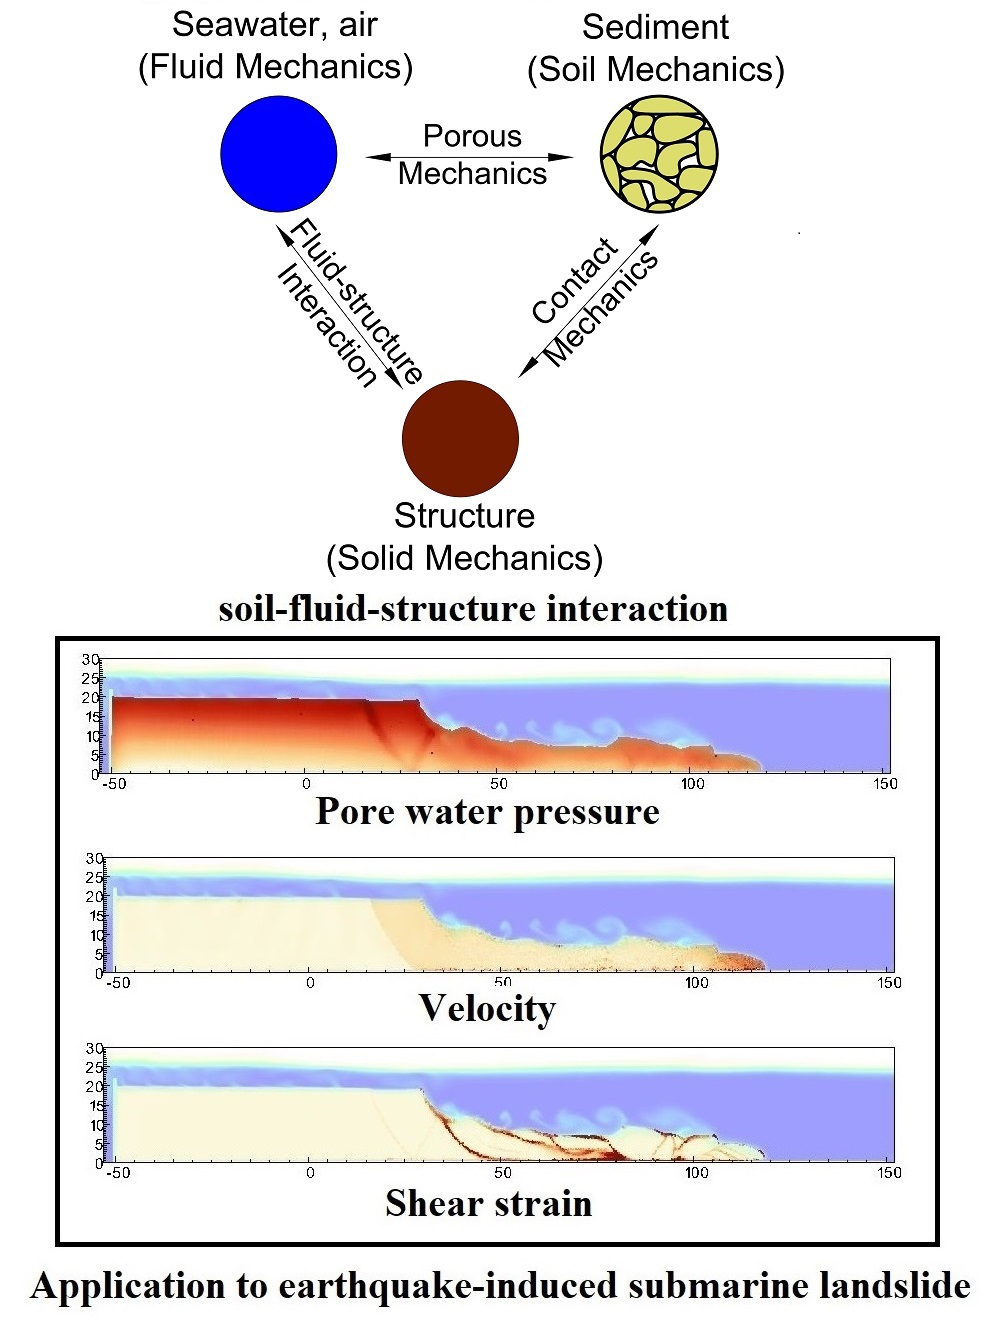
\includegraphics[scale=0.45]{abstract.jpg}
%
%
\end {graphicalabstract}

%%Research highlights
\begin{highlights}
\item MPMICE is introduced for multiphase flow in porous media.
\item Material Point method allows to model large deformation of non-isothermal porous media.
\item ICE (compressible multi-material CFD formulation) allows stabilizing pore water pressure and turbulent flow.
\item MPMICE is validated and apply to simulate the earthquake-induced submarine landslide.
\end {highlights}

\begin{keyword}
%% keywords here, in the form: keyword \sep keyword

%% PACS codes here, in the form: \PACS code \sep code

%% MSC codes here, in the form: \MSC code \sep code
%% or \MSC[2008] code \sep code (2000 is the default)
Material Point Method 
\sep MPMICE
\sep submarine landslide.
\end {keyword}
\end {frontmatter}
%
%
%
%______________________________________________________________________
%   Table of Contents    
%______________________________________________________________________
\newpage
\setcounter{secnumdepth}{-2}
\tableofcontents
%% \linenumbers

%______________________________________________________________________
\newpage
\section{\textsf{Nomenclature}}
\begin{tabular}{lll}
\\
\pmb{General variables}\\
\underline{\textsf{Variable}} & \underline{\textsf{Dimensions}} & \underline{\textsf{Description} }\\
$V$      				&   $[L^3]$     			& Representative volume\\
$n$      				&           				& Porosity\\
$\pmb{\sigma}$ 		&  $[ML^{-1}t^{-2}]$ 	& Total stress tensor\\
$\delt$       			&  $[t]$      				& Time increment\\
$\pmb{b}$ 		      &  $[ML^{1}t^{-2}]$ 	    	& Body force\\
$c_v$                   	&  $[L^2t^{-2}T^{-1}]$  	& Constant volume specific heat\\
$f_{d}$ 		  	    	&  $[MLt^{-2}]$ 			& Drag forces in momentum exchange term\\
$f^{int}$ 		  	&  $[MLt^{-2}]$ 			& Internal forces\\
$f^{ext}$ 		  	&  $[MLt^{-2}]$ 			& External forces\\
$q_{fs}$ 		  		&  $[MLt^{-2}]$ 			& Heat exchange term\\
$S$ 		  	    		&            				& Weighting function\\
$\nabla S$ 			&            				& Gradient of weighting function\\

\pmb{Solid phase}\\
\underline{\textsf{Variable}} & \underline{\textsf{Dimensions}} & \underline{\textsf{Description} }\\
$m_s   $       				&    $[M]$      		& Solid mass\\
$\rho_s$					&	$[ML^{-3}]$  	& Solid density\\
$\phi_s$				      &		  			& Solid volume fraction\\
$\overline{\rho}_s$			&	$[ML^{-3}]$  	& Bulk Solid density\\
$\pmb{x}_s$   			&  	$[L]$    			& Solid Position vector\\
$\pmb{U}_s$   			&  	$[Lt^{-1}]$    	& Solid Velocity vector\\
$\pmb{a}_s$   			&  	$[Lt^{-2}]$   	& Solid Acceleration vector\\
$\pmb{\sigma}^\prime$ 	&  	$[ML^{-1}t^{-2}]$ 	& Effective Stress tensor\\
$ \pmb{\epsilon}_s$ 	&  			 	& Strain tensor\\
$e_s$         				&  	$[L^2t^{-2}]$  	& Solid Internal energy per unit mass\\   
$T_s$           			&  	$[T]$      		& Solid Temperature\\
$\pmb{F}_s$     			&       	    			& Solid Deformation gradient\\
$V_s$     				&  	$[L^3]$      		& Solid Volume\\
\end {tabular}

\newpage
\begin{tabular}{lll}
\\
\pmb{Fluid phase}\\
\underline{\textsf{Variable}} & \underline{\textsf{Dimensions}} & \underline{\textsf{Description} }\\
$m_f   $       				&  $[M]$      				& Fluid mass\\
$\rho_f$	    		           	&   $[ML^{-3}]$  		& Fluid density\\
$\phi_f$				      &     					& Fluid volume fraction\\
$\overline{\rho}_f$			&  $[ML^{-3}]$  			& Bulk Fluid density\\
$\pmb{U}_f$   			&  $[Lt^{-1}]$    			& Fluid Velocity vector\\
$\pmb{\sigma}_f$ 			&  $[ML^{-1}t^{-2}]$ 	& Fluid stress tensor\\
$p_f$ 				&  $[ML^{-1}t^{-2}]$ 	& Fluid isotropic pressure\\
$\pmb{\tau}_f$ 			&  $[ML^{-1}t^{-2}]$ 	& Fluid shear stress tensor\\
$e_f$         				&  $[L^2t^{-2}]$  		& Fluid Internal energy per unit mass\\   
$T_f$           				&  $[T]$      				& Fluid Temperature\\
$\upsilon_f$    			&  $[L^3/M]$  			& Fluid Specific volume $\frac{1}{\rho_f}$\\
$\alpha_f$    		    		&  $[1/T]$  				& Thermal expansion\\
$\mu$    		    			&  $[ML^{-1}t^{-1}]$  	& Fluid vicousity\\
$V_f$     				&  	$[L^3]$      		& Fluid Volume\\

\pmb{Superscript}\\
\underline{\textsf{Variable}} & \underline{\textsf{Dimensions}} & \underline{\textsf{Description} }\\
$n$           			&             &    Current time step\\
$L$           			&             &    Lagrangian values\\
$n+1$         			&             &    Next time step\\
\pmb{Subscript}\\
$c$           			&             &    Cell-centered quantity\\
$p$           			&             &    Particle quantity\\
$i$           			&             &    Node quantity\\
$FC$           			&             &    Cell face quantity\\
$L, R $       			&             &    Left and Right cell faces\\
\end {tabular}


\newpage
%
%__________________________________________________
%% main text
\section{\textsf{Introduction}}

 Many geological natural processes and their interactions with man-made structures are influenced by soil-fluid-structure interactions. The prediction of these processes requires a tool that can capture complex interactions between soil, fluid, and structure, such as the process of submarine landslides. Indeed, The offshore infrastructure as well as coastal communities may be vulnerable to submarine landslides. Submarine landslides contain three stages: triggering, failure, and post-failure. Erosion or earthquakes can trigger slope failures in the first stage. Following the failure, sediments move quickly after the post-failure stage. In other words, solid-like sediments will behave like a fluid after failure. This phase transition makes the simulation of submarine landslides a challeging task.\\

Due to this phase transition, submarine landslide can be modeled by either the Computational Fluid Dynamics (CFD) or the particle-based methods. For simulating submarine slides, CFD methods solve governing equations in a full-Eulerian framework \cite{CFD1, CFD2,CFD3, CFD4} with interface capturing techniques. While CFD can handle complex flows (such as turbulent flows), it cannot account for the triggering mechanism of submarine landslides because it is not straightforward to consider 'soil constitutive laws' of sediment materials in the Eulerian framework. In contrast, particle-based methods can overcome this problem by using the Lagrangian framework. These methods have been extensively used to simulate landslides, like Material Point Method (MPM) \cite{Tran2019}, Smooth Particle Hydro Dynamics \cite{Capone2010}, Particle Finite Element Method \cite{Zhang2019}, or Coupled Eulerian Lagrangian Method \cite{Dey2016}. For simplicity, these simulations adopt total stress analysis which neglects the pore pressure development which is key factor triggering slope failures. \\

Recent developments in particle-based methods model the coupling of fluid flows in porous media by sets of Lagrangian particles. For the MPM family, it is the double-point MPM (\cite{Bandara2015, Tampubolon2017, Baumgarten2019}) where fluid particles and solid particles are overlapped in a single computational grid. Even if fluid flows are considered, particle-based methods have numerical instability in modeling the fluid flow, which requires additional numerical treatments such as the B-bar method \cite{Bandara2015}, null-space filter \cite{nullspace}, or least square approximation \cite{Zheng2021, CPLS}. Indeed, CFD is a more optimal option for complex fluid flows especially dealing with large distortions of continuum fluid media. Therefore, it could be ideal to combine the CFD with particle-based methods. More than 50 particle-based methods have been developed to solve large deformations of solids over the last two decades \cite{Chen2017}, but the MPM appears to be the best candidate for coupling with the CFD. Because MPM incorporates a stationary mesh during computation, just like CFD. As such, both MPM and CFD can be coupled naturally in a unified computational mesh.\\
%
%
\begin{figure}[h]
\center
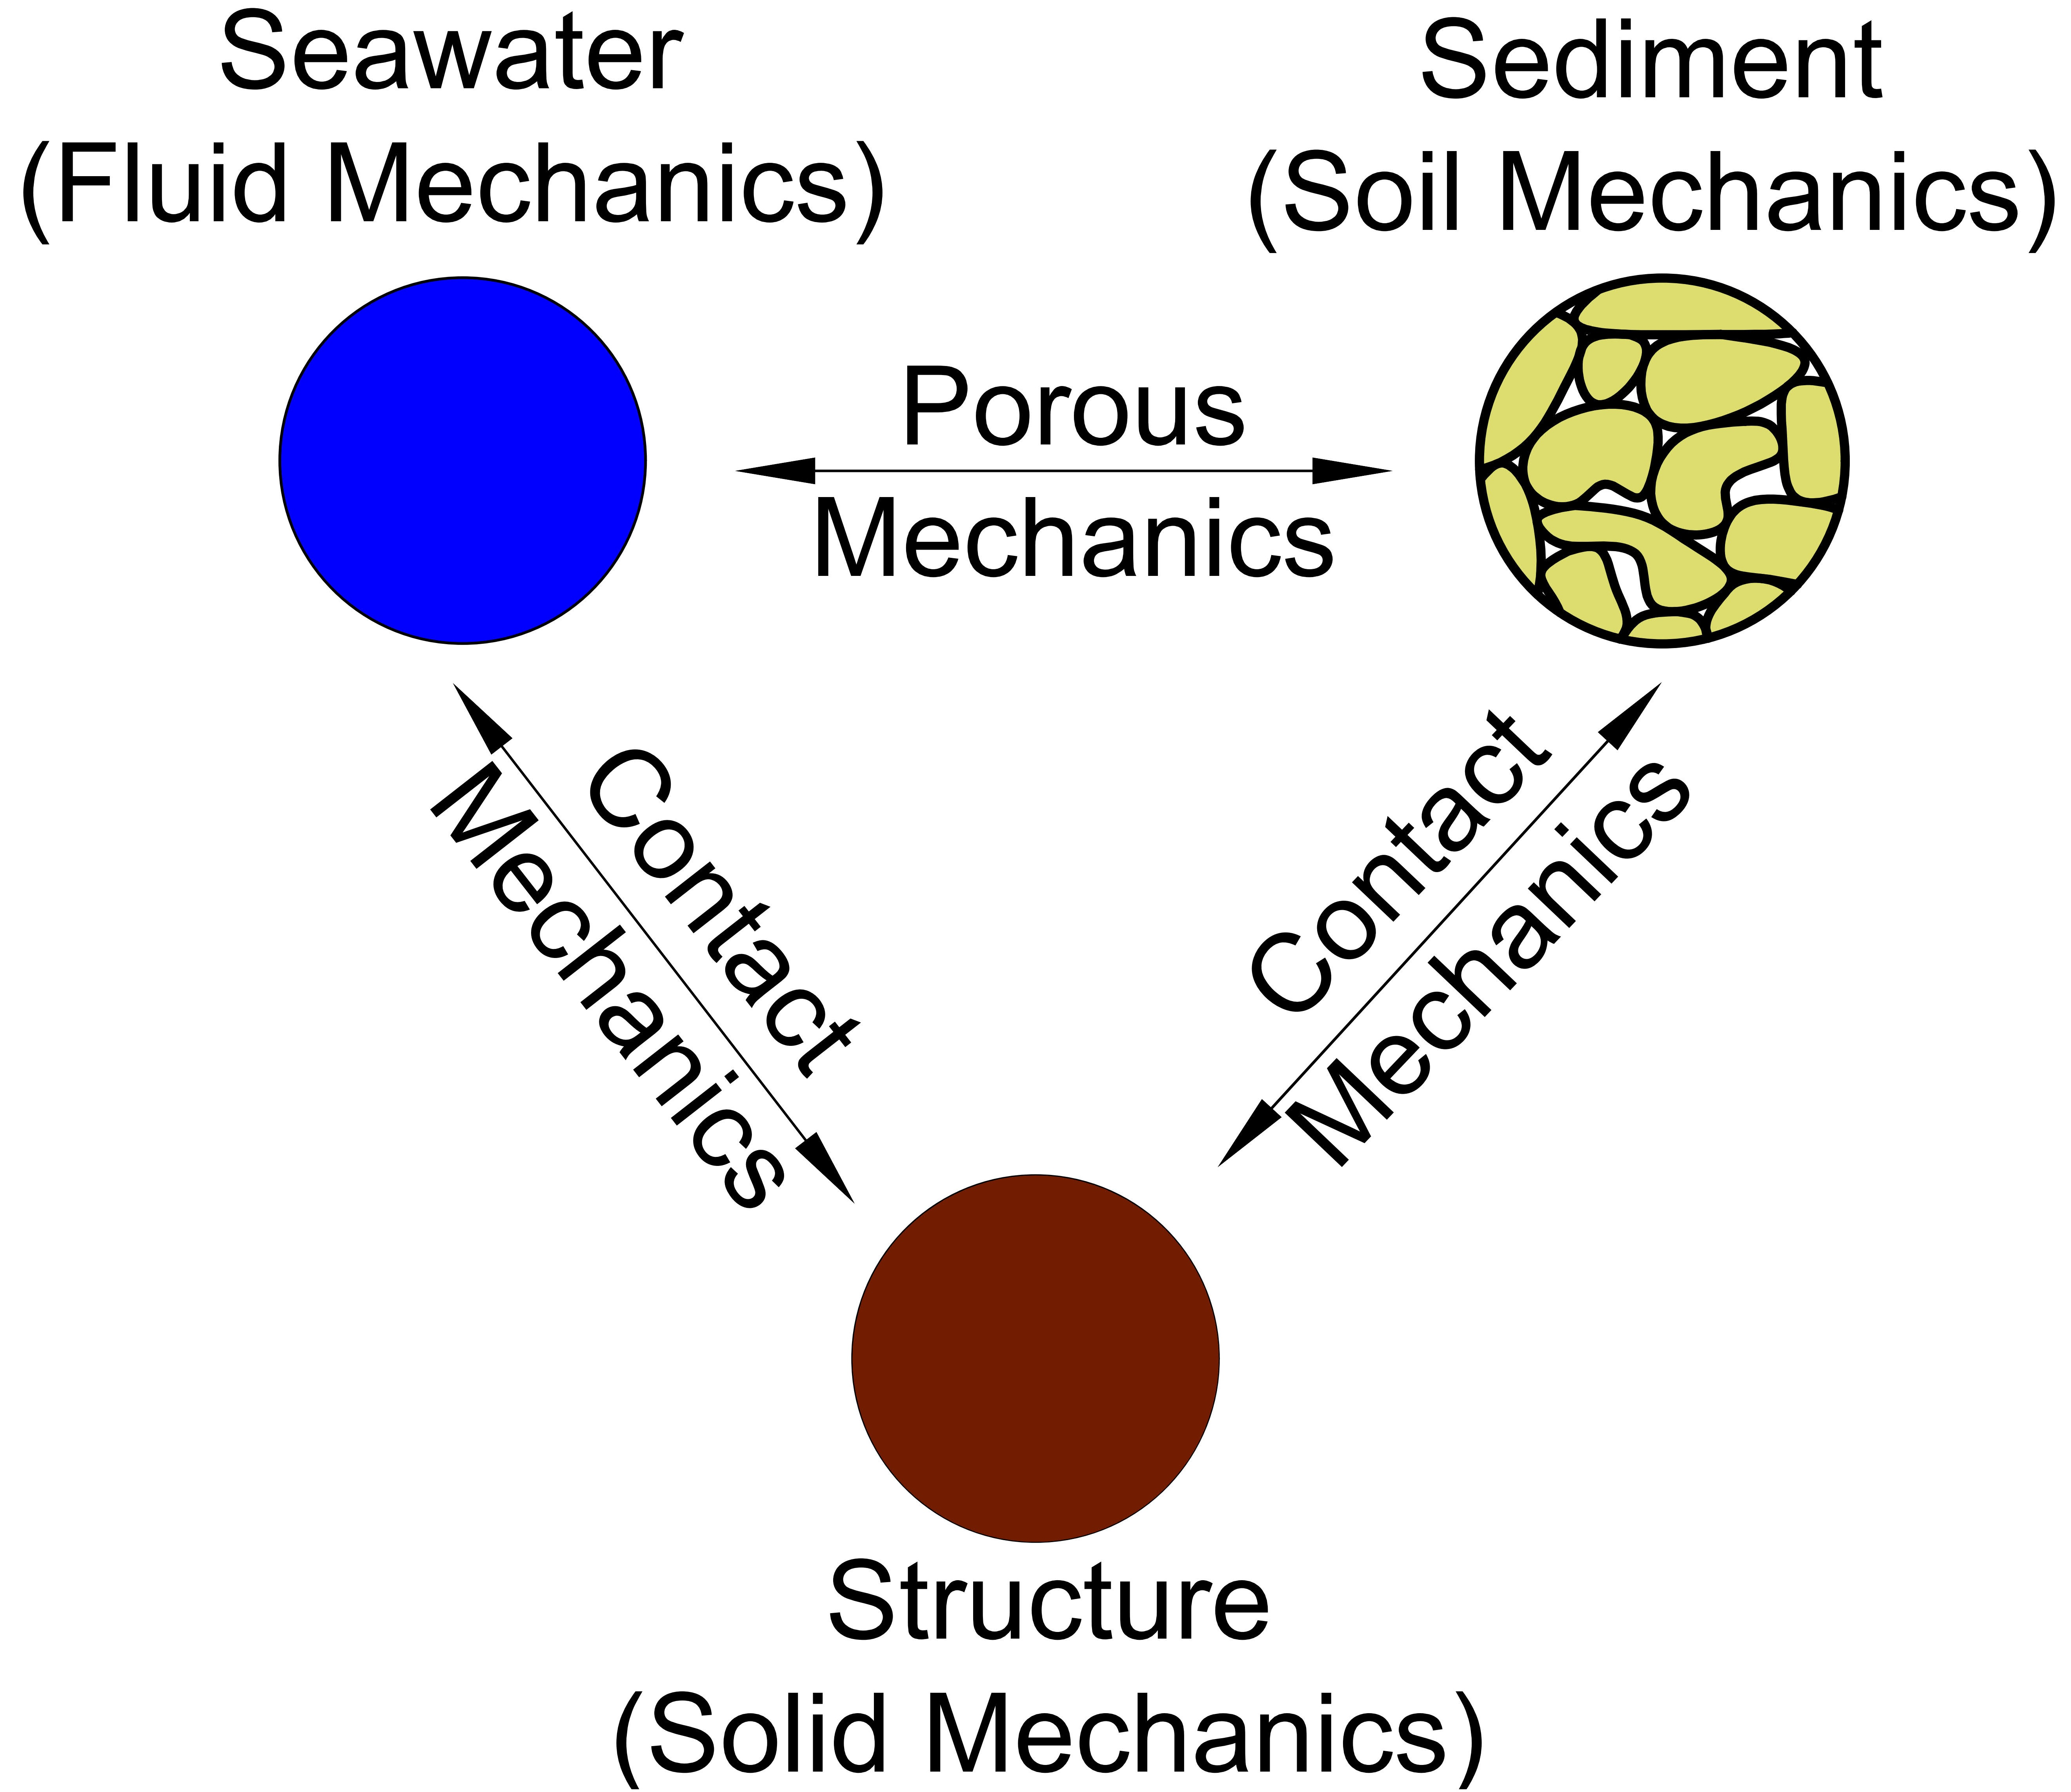
\includegraphics[scale=.3]{3phases.jpg}
\caption{Interaction between soil-fluid-structure}
\label{fig:3phases}
\end {figure}
%
%

%
%
\begin{figure}[h]
\center
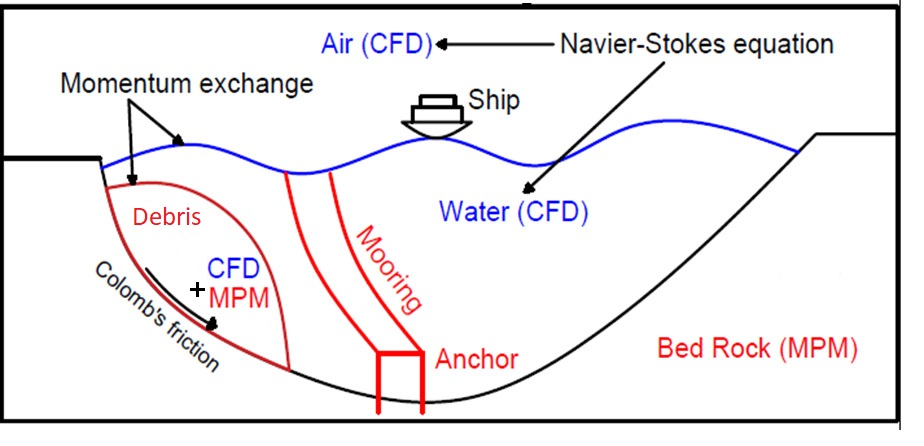
\includegraphics[scale=.4]{MPMICE.jpg}
\caption{Coupling of soil-water-structure interaction using MPMICE}
\label{fig:MPMICE}
\end {figure}
%
%

A numerical method for simulating soil-fluid-structure interaction (Figure \ref{fig:3phases}) involving large deformations, is presented in this work in order to simulate the interaction between sediment (soil), seawater (fluid) and offshore structures (structure) namely MPMICE (Figure \ref{fig:MPMICE}). In the MPMICE, the Material Point Method (MPM) is coupled with the Implicit Continuous Eulerian (ICE). The MPM method is a particle method that allows the porous soil to undergo arbitrary distortions. The ICE method, on the other hand, is a conservative finite volume technique with all state variables located at the cell center (temperature, velocity, mass, pressure). An initial technical report \cite{Kashiwa} at Los Alamos National Laboratory provided the theoretical and algorithmic foundation for the MPMICE, followed by the MPMICE development and implementation in the high-performance Uintah computational framework for simulating fluid-structure interactions \cite{MPMICE}. This paper primarily contributes further to the development of the MPMICE for analyzing the \textbf{soil}-fluid-structure interaction, since sediment should be considered as a porous media (soil) and not as a solid to capture the evolution of the pore water pressure. Baumgarten et al. \cite{Baumgarten2021} made the first attempt at coupling the Finite Volume Method with the MPM for the simulation of soil-fluid interaction. In contrast to the mentioned work, we use implicit time integration for the multi phase flows instead of explicit time integration for the single-phase flow.

%_______________________________
\section{\textsf{Theory and formulation}}
This section lay out the theoretical framework for the MPMICE model. We use the common notation of the continuum mechanics with vector and tensor denoted simply by using bold font and scalar denoted by using normal font. The notation are shown in Nomenclature.
%_______________________________
\subsection{\textsf{Assumptions}}
The following assumptions are made for the MPMICE model.
\begin{enumerate}
\item Solid phases (MPM) are described in a Lagrangian formulation while fluid phases (ICE) are described in an Eulerian formulation in the framework of continuum mechanics and mixture theory.
\item Solid grains are incompressible while the fluid phases are compressible. Solid's thermal expasion is negligible.
\item There is no mass exchange between solid and fluid phases.
\item Terzaghi's effective stress is valid. 
\end {enumerate}
%
%
%_______________________________
\subsection{\textsf{Governing equations}}
A representative element volume $\Omega$ is decomposed by two domains: solid domains $\Omega_s$ and fluid domains $\Omega_f$. Then, all domains are homogenized into two overlapping continua. Considering the volume fraction of solid $\phi_s = \Omega_s/\Omega$ and fluid $\phi_f = \Omega_f/\Omega$ with the true (or Eulerian) porosity $n=\sum{\phi_f}$ of the representative element volume, the average density of solid and fluid phases are defined as:\\
%
%
\begin{equation}
    \label{density} 
  \overline{\rho}_s   = \phi_s \rho_s, \qquad  \overline{\rho}_f   = \phi_f \rho_f \quad
\end {equation}
%
%
The mass of solid and fluid phases are:\\
%
%
\begin{equation}
    \label{mass} 
  m_s   = \int_{\Omega_s} \rho_s dV = \overline{\rho}_s V, \qquad  m_f   = \int_{\Omega_f} \rho_f dV = \overline{\rho}_f V
\end {equation}
%
%
Reviewing the Terzaghi's effective stress concept for the saturated porous media, the total stress $\pmb{\sigma}$ is calculated by:\\
%
%
\begin{equation}
    \label{Terzaghi} 
  \pmb{\sigma}   = \pmb{\sigma}^\prime -p_f\pmb{I}
\end {equation}
%
%
The balance equations are derived based on the mixture theory. The representative thermodynamic state of the fluid phases are given by the vector $[m_f,\pmb{U}_f,e_f,T_f,\upsilon_f]$ which are mass, velocity, internal energy, temperature, specific volume. The representative state of the solid phases are given by the vector $[m_s,\pmb{U}_s,e_s,T_s,\pmb{\sigma}^\prime,p_f]$ which are mass, velocity, internal energy, temperature, effective stress and pore water pressure. The derivation is presented in detail in the Appendix. \\
%
%_______________________________
% mass
%_______________________________
\underline{\hspace{5in}}\\
\underline{\textsf{Mass Conservation}}\\
The mass balance equations for both fluid (e.g., water, air) and solid phases are:\\
%
%
\begin{equation}
    \label{massbalance}
   \frac{1}{V}\frac{\partial m_f}{\partial t} + \nabla \cdot  (m_f \pmb{U}_f)= 0, \\ 
   \frac{1}{V}\frac{D_sm_s}{Dt} = 0    
\end {equation}
%
Solving the mass balance equation leads to:
%
%
\begin{equation}
  \frac{D_s n}{Dt} = \phi_s \nabla \cdot \pmb{U}_s  
\end {equation}
%
%
%_______________________________
% momentum
%_______________________________
\underline{\hspace{5in}}\\
\underline{\textsf{Momentum Conservation}}\\
The momentum balance equations for the fluid phases (e.g., water, air) are:
%
%
\begin{equation}
     \frac{1}{V} \left[ \frac{\partial (m_f \pmb{U}_f)}{\partial t} + \nabla \cdot  (m_f \pmb{U}_f \pmb{U}_f) \right] = - \phi_f \nabla p_f  +  \nabla \cdot \pmb{\tau}_f + \overline{\rho}_f \pmb{b} +  \sum \pmb{f}_{d}
\end {equation}
%
%
The momentum balance equations for the solid phases are:
%
%
\begin{equation}
     \frac{1}{V}\frac{D_s(m_s \pmb{U}_s)}{Dt} = 
    \nabla \cdot (\pmb{\sigma}^\prime) - \phi_s \nabla p_f 
    + \overline{\rho}_s \pmb{b} +  \sum \pmb{f}_{fric}    -  \sum \pmb{f}_{d}
\end {equation}
%
%
%_______________________________
% Energy
%_______________________________
\underline{\hspace{5in}}\\
\underline{\textsf{Energy Conservation}}\\
The internal energy balance equations for the fluid phases (e.g., water, air) are:
%
%
\begin{equation}
    \label{fluidenergy}
     \frac{1}{V} \left[ \frac{\partial (m_f e_f)}{\partial t} + \nabla \cdot  (m_f e_f \pmb{U}_f) \right]  = 
    -\overline{\rho}_f p_f  \frac{D_f\upsilon_f}{Dt} + \pmb{\tau}_f : \nabla \pmb{U}_f + \nabla \cdot \pmb{q}_f +  \sum q_{sf}
\end {equation}
%
%
The internal energy balance equations for the solid phase are:
%
%
\begin{equation}
    \label{solidenergy}
     \frac{m_s}{V}  c_v \frac{D_s( T_s)}{Dt} = \pmb{\sigma}^\prime: \frac{D_s( \pmb{\epsilon}_s^p)}{Dt} + \nabla \cdot \pmb{q}_s -  \sum q_{sf} 
\end {equation}
%
%
where $c_v$ is the specific heat at constant volume of the solid materials.
\underline{\hspace{5in}}\\
Closing the systems of equations, the following additional models are needed: \\
(1) A constitutive equation to describe the stress - strain behaviour of solid phase (computing effective stress $\pmb{\sigma}^\prime$). \\
(2) Optional turbulent model to compute the viscous shear stress $\pmb{\tau}_f$.\\
(3) Frictional forces $\pmb{f}_{fric}$ for the contact for soil-structure interaction between solid/porous materials with the friction coefficient $\mu_{fric}$. \\
(4) Exchange momentum models (computing drag force $\pmb{f}_{d}$) for interaction between materials. \\
(5) Energy exchange models (computing temerature exhange term $q_{sf}$) for interaction between materials. \\
(6) An equation of state to establish relations between thermodynamics variables of each fluid materials $[P_{f}, \overline{\rho}_f, \upsilon_f, T_f, e_f]$. \\
Four thermodynamic relations for the equation of states are:
%
%
\begin{equation}
\begin{gathered}
  e_f =  e_f (T_f, \upsilon_f)\\
 P_f =  P_f(T_f, \upsilon_f)\\
  \phi_f = \upsilon_f \overline{\rho}_f\\
  0 = n - \sum_{f=1}^{N_f} \upsilon_f \overline{\rho}_f\\
\end {gathered}
\end {equation}
%
%
%_______________________________
\subsubsection{Constitutive soil model}
As a result of the explicit MPM formulation, we can derive the constitutive law in the updated Lagrangian framework of "small strain - large deformation". Therefore, the rotation of the particles (representative element volume) is manipulated by rotating the Cauchy stress tensor. First, the deformation gradient is decomposed into the polar rotation tensor $\pmb{R}_s^{n+1}$ and stretch tensor $\pmb{V}_s^{n+1}$ as:
%
%
\begin{equation}
     \pmb{F}_s^{n+1} = \pmb{V}_s^{n+1} \pmb{R}_s^{n+1}
\end {equation}
%
%
Then, before calling the constitutive model, the stress and strain rate tensor are rotated to the reference configuration as:
%
%
\begin{equation}
     \pmb{\sigma}^{\prime,n*} =  (\pmb{R}_s^{n+1})^T \pmb{\sigma}^{\prime,n*} \pmb{R}_s^{n+1}
\end {equation}
%
%
\begin{equation}
    \delta \pmb{\epsilon}^{n*} =  (\pmb{R}_s^{n+1})^T \delta \pmb{\epsilon}_s^{n*} \pmb{R}_s^{n+1}
\end {equation}
%
%
Using the constitutive model with the input tensors $\pmb{\sigma}^{\prime,n*}, \delta \pmb{\epsilon}^{n*}$ to compute the Cauchy stress tensor at the advanced time step $\pmb{\sigma}^{\prime,n+1*}$ then rotating it back to current configuration as:
%
%
\begin{equation}
    \pmb{\sigma}^{\prime,n+1} =  \pmb{R}_s^{n+1} \pmb{\sigma}^{\prime,n+1*} (\pmb{R}_s^{n+1})^T
\end {equation}
%
%
In this paper, we adopt the hyper-elastic Neo Hooken model for the structure materials and additionally Mohr-Coulomb failure criteria for the soil (porous media) materials. The Cauchy stress of the hyper-elastic Neo Hookean model can be written as:
%
%
\begin{equation}
    \pmb{\sigma}^{\prime} =  \frac{ \lambda ln(J)}{J} + \frac{\mu}{J} (\pmb{F} \pmb{F}^T - \pmb{J})
\end {equation}
%
%
where $\lambda$ and $\mu$ are bulk and shear modulus ad J is the determinant of the deformation gradient $\pmb{F}$. And the yield function f and flow potentials g of the Mohr-Coulomb can be written as:
%
%
\begin{equation}
\begin{gathered}
   f =  \sigma_1^{\prime} -  \sigma_3^{\prime} -2c^{\prime} cos(\phi^{\prime}) - (\sigma_1^{\prime} +  \sigma_3^{\prime})sin(\phi^{\prime})\\
   g =  \sigma_1^{\prime} -  \sigma_3^{\prime} -2c^{\prime} cos(\psi^{\prime}) - (\sigma_1^{\prime} +  \sigma_3^{\prime})sin(\psi^{\prime})
\end {gathered}
\end {equation}
%
%
where the $c^{\prime}$, $\phi^{\prime}$ and $\psi^{\prime}$ are cohesion and friction angle and dilation angle. $\sigma_1^{\prime}$ and $\sigma_3^{\prime}$ are maximum and minimum principal stress.
%_______________________________
\subsubsection{Turbulent model}
The turbulent effect is modelled using a statistical approach namely large-eddy simulation. In this approach, the micro-scale turbulent influence in the dynamics of the macro-scale motion is computed through simple models like Smagorinsky model. In the Smagorinsky model, the residual stress tensor is:
%
\begin{equation}
     \tau_{ij} = 2 \mu_{eff} (\overline{S}_{ij} - \frac{1}{3} \delta_{ij} \overline{S}_{kk}) + \frac{1}{3} \delta_{ij} \tau_{kk}
\end {equation}
%
%
where the the strain rate tensor is given by:
%
\begin{equation}
     \overline{S}_{ij} = \frac{1}{2} (\frac{\delta \overline{\pmb{U}}_i}{\delta x_j} + \frac{\delta \overline{\pmb{U}}_j}{\delta x_i})
\end {equation}
%
%
and the effective viscosity is sum of molecular viscosity and turbulent viscosity $\mu_{eff} = \mu + \mu_t$ in which the turbulent viscosity $\mu_t$ is calculated by:
%
\begin{equation}
    \mu_t = (C_s \triangle)^2 \sqrt{2 \overline{S}_{ij} \overline{S}_{ij}}
\end {equation}
%
%
where $C_s$ is the Smagorinsky constant with the value of 0.1 and $\triangle = \sqrt[3]{dx dy dz}$ is the grid size that defines the subgrid length scale.
%_______________________________
\subsubsection{Frictional force for soil-structure interaction}
MPMICE includes a contact law for the interaction between soil and structure using the first Coulomb friction contact for MPM presented by Bardenhagen et al. (\cite{MPMcontact}).  The magnitude of the friction force at the contact depends on the friction coefficient $\mu_{fric}$ and the normal force  $ \pmb{f}_{norm}$  computed from the projection of the contact force  in the normal direction.
%
\begin{equation}
   \pmb{f}_{fric} = \mu_{fric}  \pmb{f}_{norm}
\end {equation}
%
%
The contact determines whether the soil is sliding or sticking to the structure by comparing the friction force with the sticking force $\pmb{f}_{stick}$  computed from the projection of the contact force in the tangent direction as:
%
\begin{equation}
\begin{gathered}
\textrm{   if    }    \pmb{f}_{fric} \geq  \pmb{f}_{stick}   \textrm{    no sliding    } \\
\textrm{    if    }   \pmb{f}_{fric} <   \pmb{f}_{stick}   \textrm{    sliding occurs    }  
\end {gathered}
\end {equation}
Frictional sliding between solid materials also generates dissipation and the work rate generated from the sliding can be calculated as:
%
\begin{equation}
   \Delta W_{friction} = \pmb{f}_{fric} d
\end {equation}
%
%
where d is the sliding distance which can computed based on the sliding velocity between two materials. 
%_______________________________
\subsubsection{Momentum and Energy exchange model}
Currently, the energy exchange coefficient $H_{sf}$ is assumed to be constant for the sake of simplicity. Then the energy exchange can be written as:
%
%
\begin{equation}
     q_{sf} = H_{sf} (T_f -T_s)
\end {equation}
%
%
On the other hand, the drag force can be calculated as:
%
%
\begin{equation}
    f_{d} = K (\pmb{U}_s - \pmb{U}_f)  
\end {equation}
%
%
For the momentum exchange between fluid flows and porous media, we assume that the drag force $\pmb{f}_{d}$ depends on the average grain size of the grains $D_p$, the porosity $n$, the fluid viscosity $\mu_f$, and is proportional to the relative velocities of soil grains and fluid $(\pmb{U}_s - \pmb{U}_f)$. Based on recent investigation of CFD simulations of fluid flow around mono- and bi-disperse packing of spheres for $0.1 < \phi_s < 0.6$ and $Re < 1000$ \cite{Drag}. The drag force is given by: \\
%
%
\begin{equation}
     \pmb{f}_{d} = \frac{18\phi_s(1-\phi_s)\mu_f}{D_p^2} F(\phi_s, Re) (\pmb{U}_s - \pmb{U}_f)  
\label{fd}
\end {equation}
%
%
where Reynolds number $Re$ are computed as:
%
%
\begin{equation}
     Re = \frac{n \rho_f D_p}{\mu_f} |\big\|(\pmb{U}_s - \pmb{U}_f)\big\|
\end {equation}
%
%
The function $F(\phi_s, Re)$ can be calculated as:
%
%
\begin{equation}
     F(\phi_s, Re)  = F(\phi_s, 0)  + \frac{0.413Re}{24 (1-\phi_s)^2} (\frac{(1-\phi_s)^{-1}+3\phi_s(1-\phi_s)+8.4Re^{-0.343}}{1+10^{3\phi_s}Re^{-(1+4\phi_s)/2}})
\end {equation}
%
%
where the low Reynold coefficient $ F(\phi_s, Re\rightarrow0)$ is:
%
%
\begin{equation}
     F(\phi_s, 0)  = \frac{10\phi_s}{ (1-\phi_s)^2}+(1-\phi_s)^2(1+1.5\sqrt{\phi_s})
\end {equation}
%
%
When validating the model with analytical solution, it requires to know the hydraulic conductivity $K$. In such case, we convert the equation (\ref{fd}) to Kozeny-Carman formula by assuming $F(\phi_s, Re) = 10\phi_s/(1-\phi_s)^2$, leading to 
%
%
\begin{equation}
     \pmb{f}_{d} = \frac{180 \phi_s^2\mu_f}{D_p^2 (1-\phi_s)} (\pmb{U}_s - \pmb{U}_f)  
\label{fd}
\end {equation}
%
%
Then, the draging force following the Darcy law is given by:
%
%
\begin{equation}
     \pmb{f}_{d} =  \frac{n^2 \mu_f}{ \kappa}(\pmb{U}_s - \pmb{U}_f)  
\end {equation}
%
%
where $\kappa$ being intrinsic permeability of soil which can be written as:
%
%
\begin{equation}
     \kappa  =  \frac{K \mu_f}{\rho_f  g}
\end {equation}
%
%
As such, the hydraulic conductivity will be expressed as:
%
%
\begin{equation}
    K = \frac{D_p^2 (1-\phi_s)^3}{180 \phi_s^2 \mu_f} \rho_f  g
\end {equation}
%
%

\subsubsection{Solving momentum and energy exchange with an implicit solver}
%
%
\begin{figure}[h]
\center
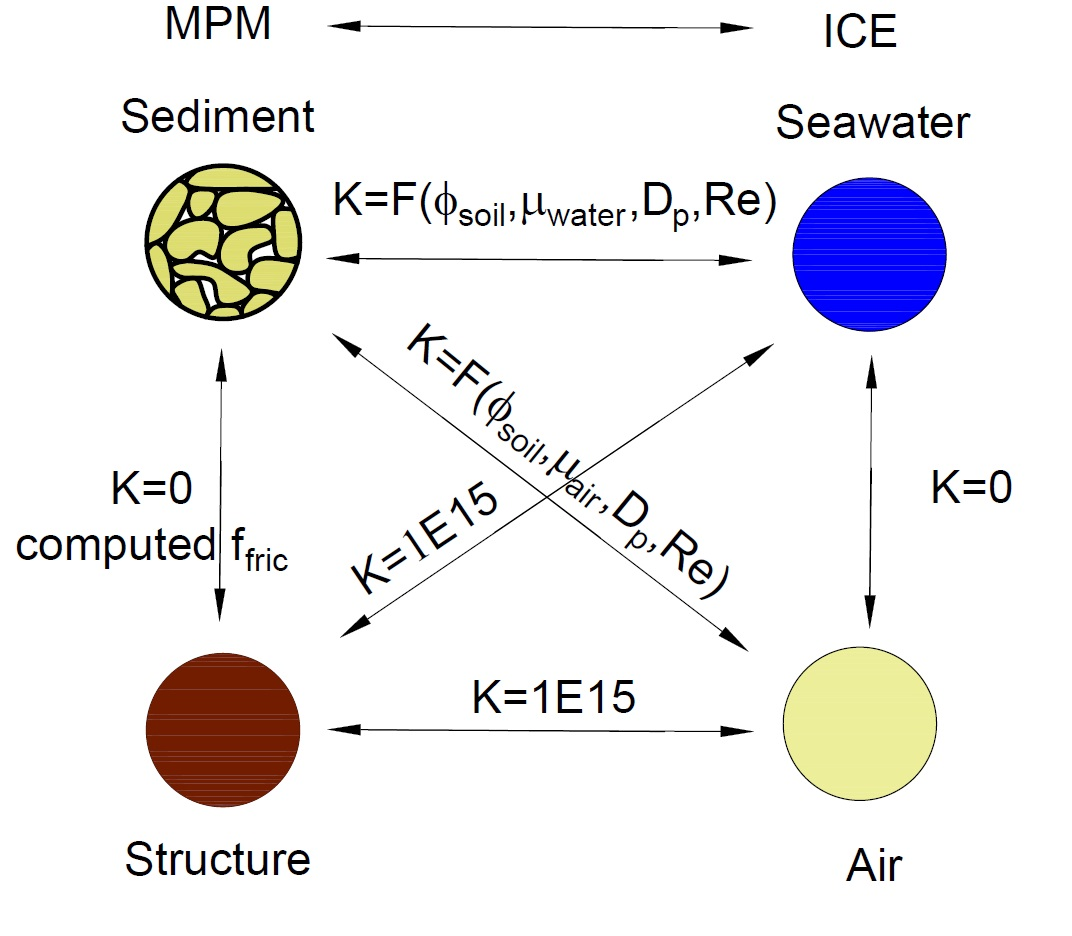
\includegraphics[scale=1.0]{K.jpg}
\caption{Momentum exchange coefficient between materials}
\label{fig:K}
\end {figure}
%
%
The derivation of the implicit integration for the momentum exchange is presented in the Appendix's section 'Momentum and energy exchange with an implicit solver'. The linear equations for multi phases i,j=1:$N$
has the form as:
%
\[ \begin{vmatrix} (1 + \beta_{ij})  &  -\beta_{ij} \\
                  -\beta_{ji}       &  (1 + \beta_{ji})
    \end {vmatrix}
    \begin{vmatrix} \Delta \pmb{U}_{i} \\
                    \Delta \pmb{U}_{j}
    \end {vmatrix}
    =
    \begin{vmatrix}  \beta_{ij}(\pmb{U}_{i}^{*} - \pmb{U}_{j}^{*}) \\
                    \beta_{ji}(\pmb{U}_{i}^{*} - \pmb{U}_{j}^{*})
    \end {vmatrix}                
\]
%
%
where the intermediate velocity for fluid phases f=1:$N_f$ and for solid/porous phases s=1:$N_s$ can be calculated by:
%
\begin{equation}
\begin{gathered}
\pmb{U}_{f}^{*} = \pmb{U}_{f}^{n} + \delt (-\frac{\nabla P_{f}^{n+1}}{\rho_f^n}  + \frac {\nabla \cdot \pmb{\tau}_f^{n}}{\overline{\rho}^n_{f}} + \pmb{b}) \\
\pmb{U}_{s}^{*} = \pmb{U}_{s}^{n} + \delt (\frac{\nabla \cdot \pmb{\sigma}^{'n}}{\overline{\rho}^n_{s}}    - \frac{\nabla P_{f}^{n+1}}{\rho_s}  + \pmb{b})
\end {gathered}
\end {equation}
%
%
Also, the momentum exchange coefficient can be computed at every time step as $\beta_{12} = K/\overline{\rho}_{f}^n$ and $\beta_{21} = K/\overline{\rho}_{s}^n$ with the coefficient depending on the different type of interactions (see Figure \ref{fig:K}) as for example: \\
\begin{enumerate}
\item The drag force is set to zero in soil-structure interactions, and instead the frictional force is computed.
\item As a result of fluid-structure interaction, the momentum exchange coefficient should be extremely high (1E15) when the solid material points are considered to be zero-porosity/zero-permeability.
\item In the case of soil-fluid interaction, the drag force is calculated using the equation (\ref{fd}). Considering that air has a much lower viscosity than water, its drag force is much lower than the drag force of water in a pore.
\item A momentum exchange coefficient of 1E5 is applied between multiphase flows. This value is far higher than reality \cite{Stewart1974}, but it is necessary to have enough numerical stability to conduct simulations in the numerical example.
\end {enumerate}
Similar approach applied for the ernergy exchange term leading to:
%
%
\[ \begin{vmatrix} (1 + \eta_{ij})  &  -\eta_{ij} \\
                  -\eta_{ji}       &  (1 + \eta_{ji})
    \end {vmatrix}
    \begin{vmatrix} \Delta T_{i} \\
                    \Delta T_{j}
    \end {vmatrix}
    =
    \begin{vmatrix}  \eta_{ij}(T_{i}^{n} - T_{j}^{n}) \\
                    \eta_{ji}(T_{j}^{n} - T_i^{n})
    \end {vmatrix}                
\]
with $\eta$ being the energy exchange coefficient.
%_______________________________
\subsubsection{Equation of state for fluid plases}
%
%
\begin{figure}[H]
\center
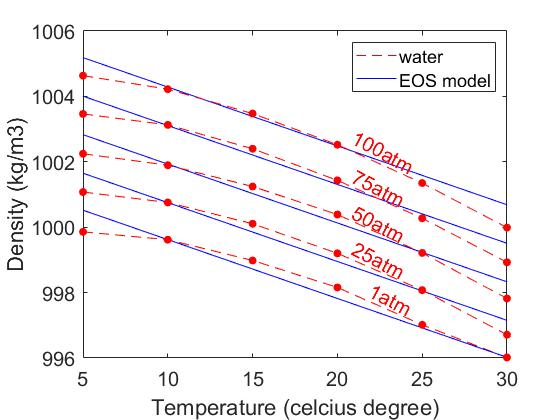
\includegraphics[scale=.5]{water1.jpg}
\caption{Equation of state of water}
\label{fig:water1}
\end {figure}
%
%
The equation of state establishes relations between thermodynamics variables $[P_f, \rho_f, T_f]$. The choice of the equation of state depends on the types of the fluid materials. For example, for the air, it is possible to assume the equation of state for the perfect gas which obeys:
%
%
\begin{equation}
    P_f = \rho_f R T_f
\end {equation}
%
%
where $R$ is the gas constant. For the water, a simple linear equation of state is in the following form:
%
%
\begin{equation}
    P_f = P_{ref} + K_f (\rho_f - \rho_{ref} - \alpha_f(T_f - T_{ref}))
\label{waterEOS}
\end {equation}
%
%
where reference pressure $P_{ref}$ = 1 atm = 101325 Pa, reference temperature $T_{ref}$ = 10°C, reference density  $\rho_{ref}$ = 999.8 kg/m3, the bulk modulus of water $K_f$ = 2 GPa, and the water thermal expansion $\alpha_f$ = 0.18 °$C^{-1}$. Equation (\ref{waterEOS}) matches well with the state of the water (see Figure \ref{fig:water1}).

%_______________________________
\section{\textsf{Numerical implementation}}
\label{Discretization}
%
%
\begin{figure}[H]
\center
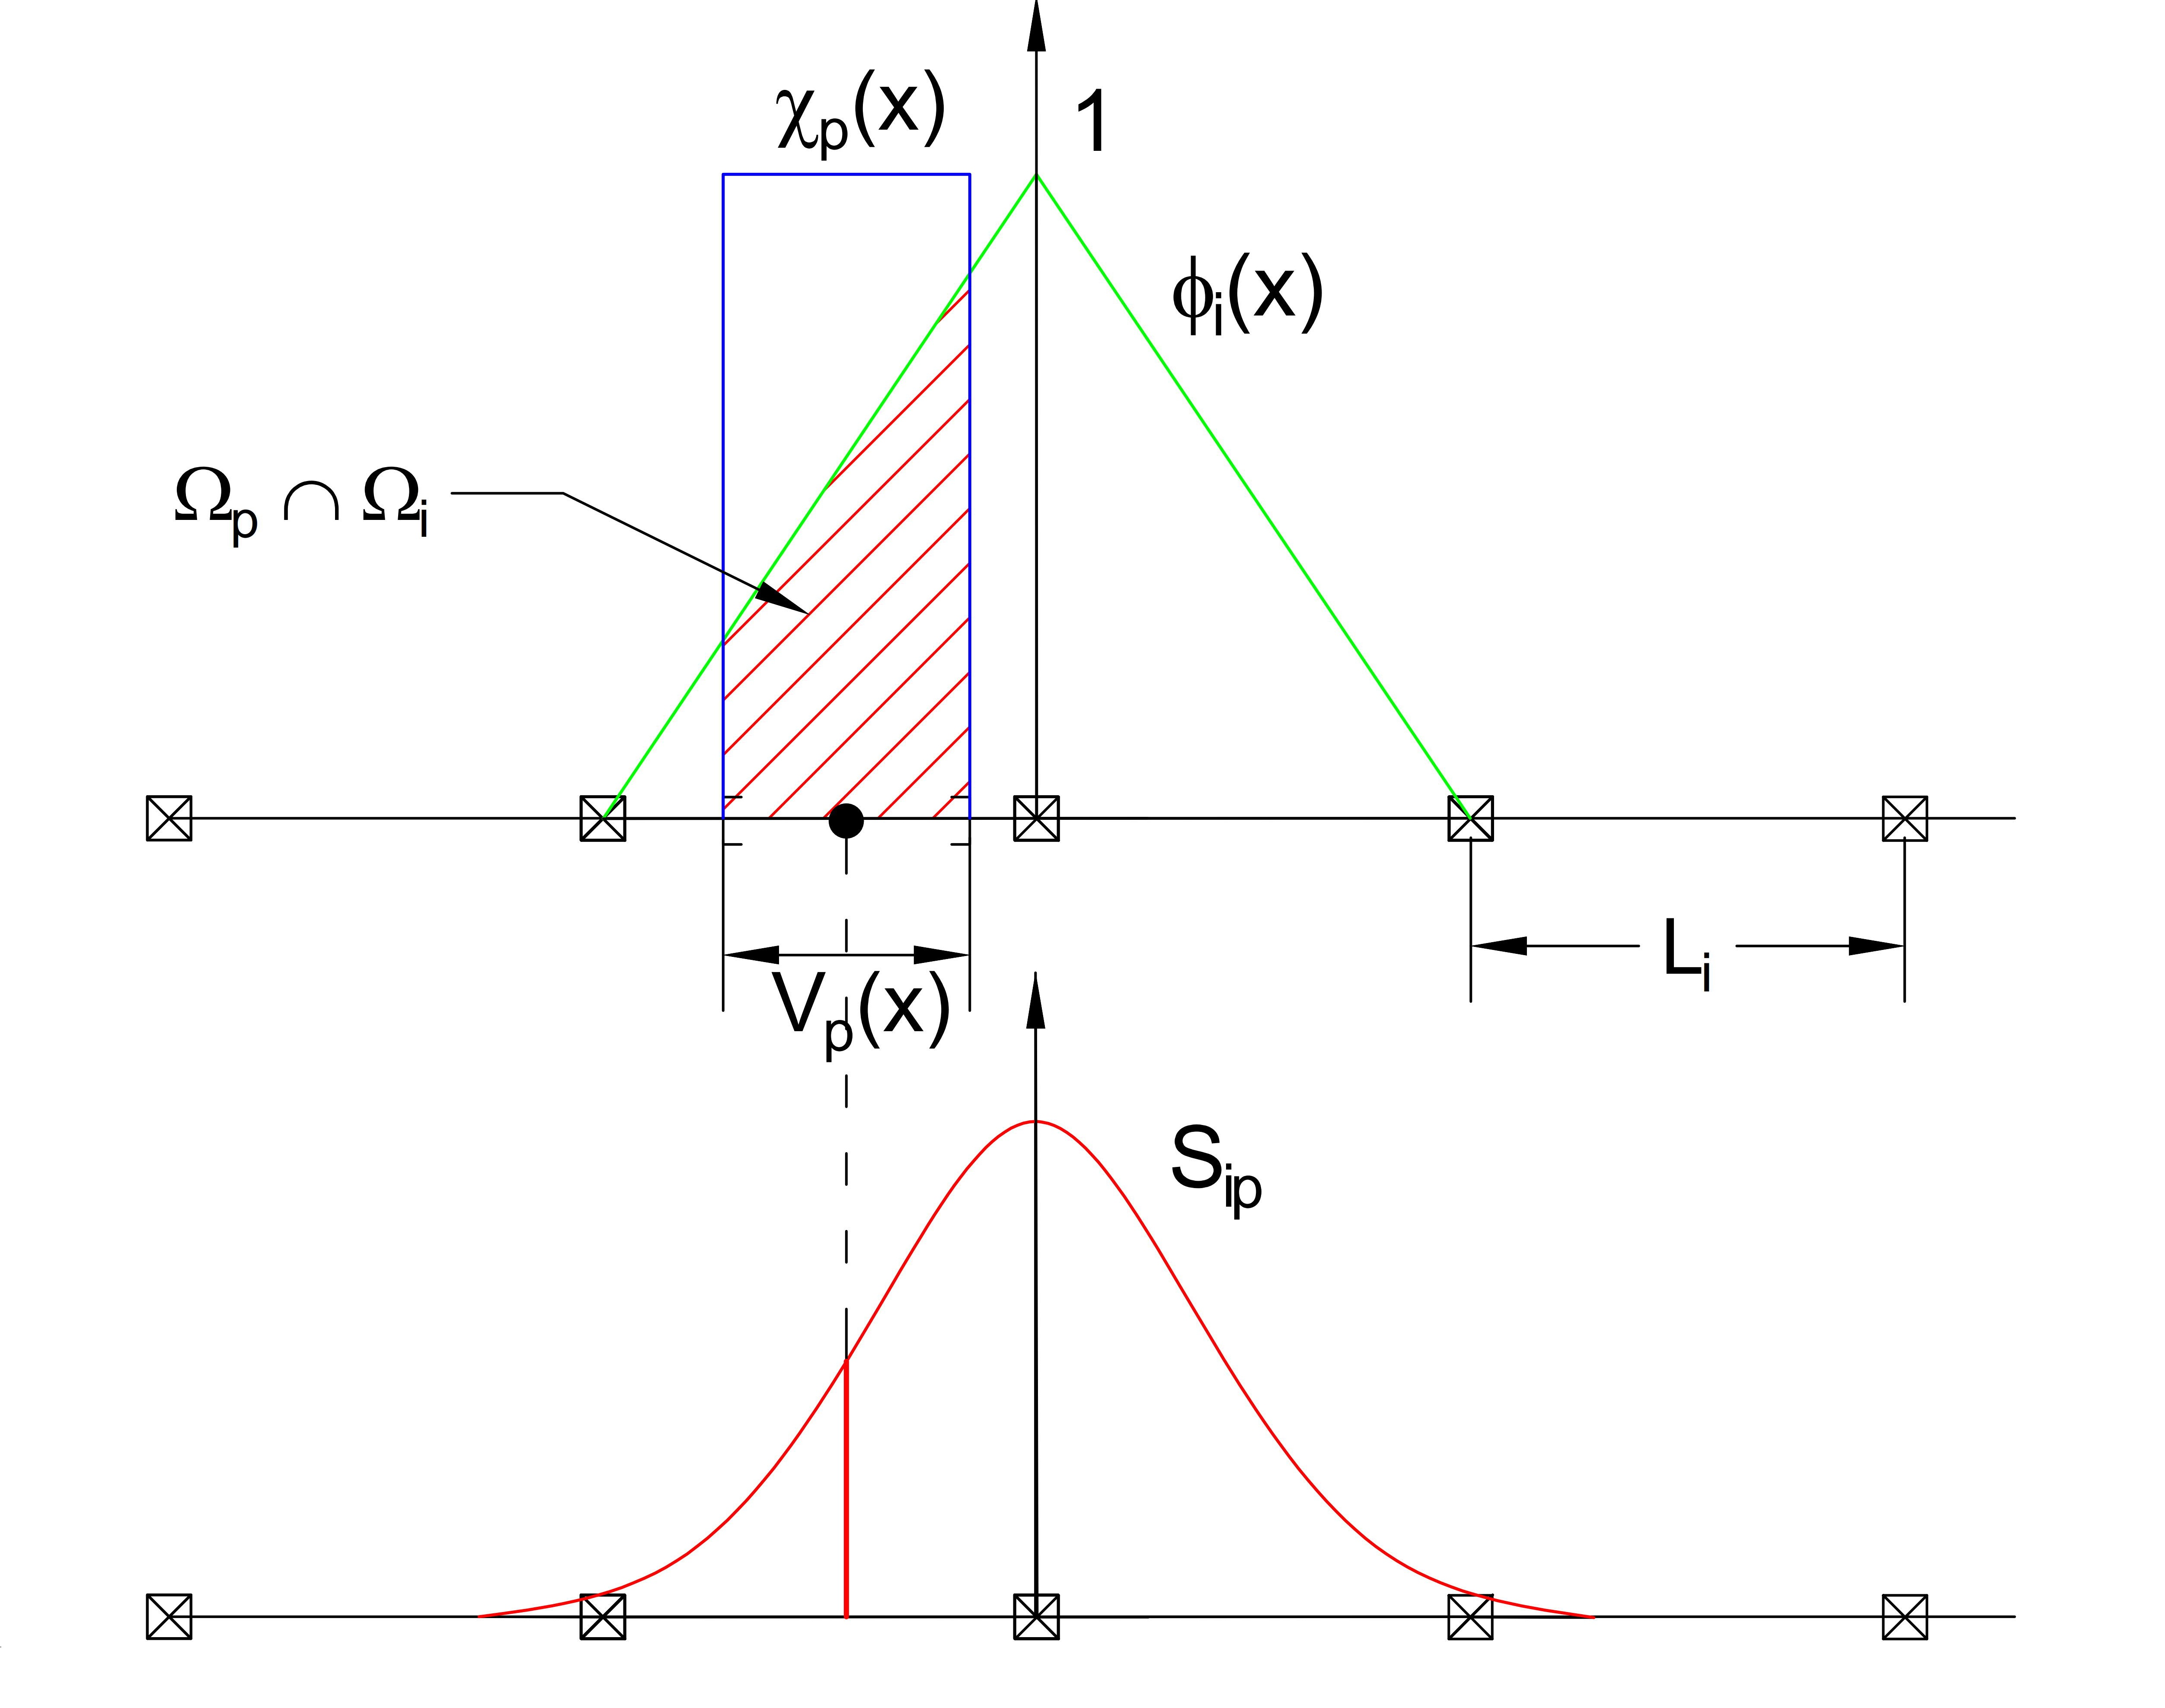
\includegraphics[scale=.5]{GIMPshape.jpg}
\caption{GIMP weighting function (red as a convolution of the linear basis shape function (green) and the characteristic function (blue)}
\label{fig:GIMP}
\end {figure}
%
The fluid phases are discretized in the grid with the state variables stored at the centroid of the cells $[\rho_{f,c},\pmb{U}_{f,c},T_{f,c},\upsilon_{f,c}]$ while the solid phase is discretized in the particles with the state variables $[m_{sp},\pmb{U}_{sp},T_{sp},\pmb{\sigma}^\prime_{sp}]$. In the Material Point Method, we use the generalized interpolation technique \cite{GIMP} using the weight function as a convolution of a grid shape function $N_i(\pmb{x})$ in a nodal domain $\Omega_i$ and a characteristic function $\chi_p (\pmb{x})$ in a particle domain $\Omega_p$ with the volume $V_p (\pmb{x})$ as follows:
%
%
\begin{equation}
     S_{ip} = \frac {1}{V_p} \int_{\Omega_i \cap \Omega_p} N_i(\pmb{x}) \chi_p (\pmb{x}) d\pmb{x}
\end {equation}
%
%
where the volume $V_p (\pmb{x})$ of the material point p can be calculated as:
%
%
\begin{equation}
     V_{p} = \int_{\Omega_p} \chi_p (\pmb{x}) d\pmb{x}
\end {equation}
%
The characteristic function is the Heaviside function as $\chi_p = 1  \text{  if  } \pmb{x} \in \Omega_p$, otherwise 0 (see Figure \ref{fig:GIMP}). For the interpolation of the centroid of the cell, the linear basis function is used as:
%
\begin{equation}
     S_{ci}  = N_i(\pmb{x_c}) 
\end {equation}
%
The time discretization are solved using the following steps.
%
%
\begin{sidewaysfigure}
\center
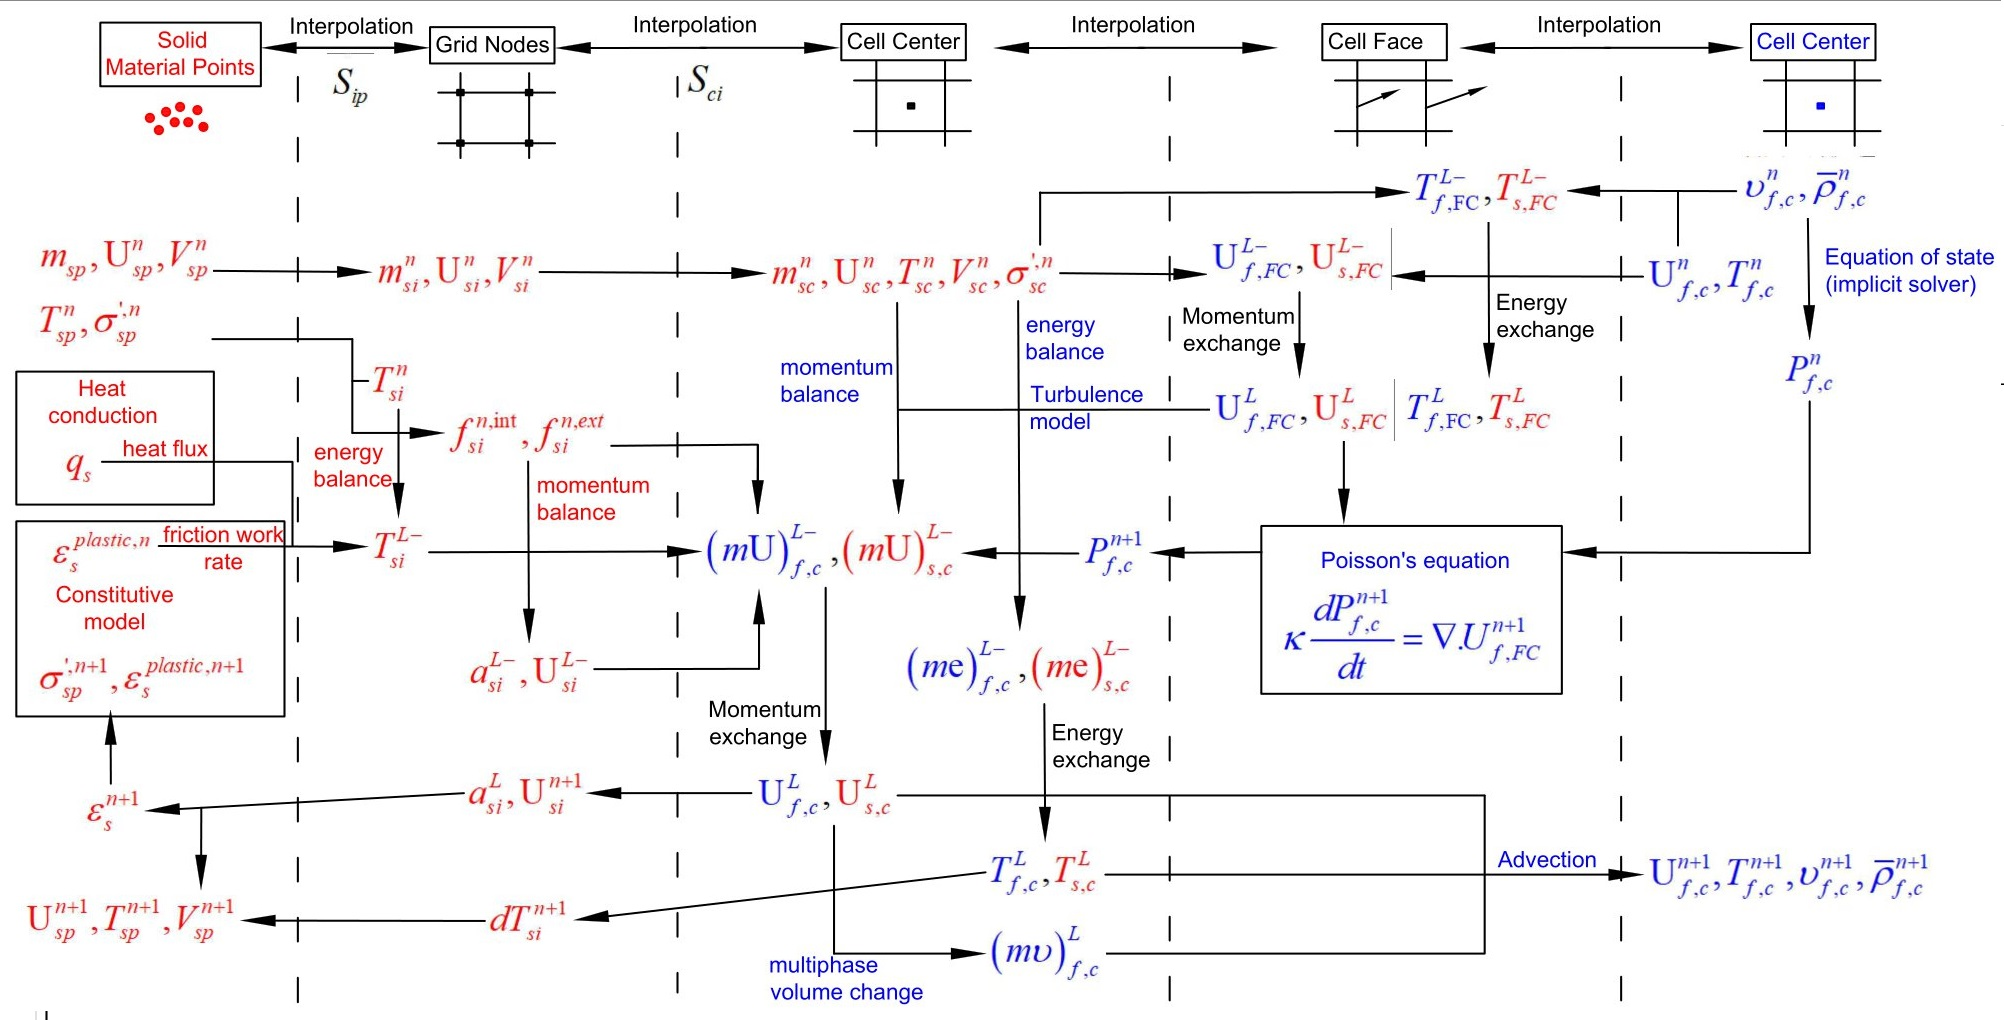
\includegraphics[scale=0.9]{MPMICE_chart.jpg}
\caption{Numerical implementation of MPMICE}
\label{fig:MPMICE_chart}
\end {sidewaysfigure}
%
%
\subsection{\textsf{Interpolation from Solid Particle to Grid}}
%
%
The nodal values of the solid state (mass, velocity, temperature, volume) are:
%
%
\begin{equation}
\begin{gathered}
     m_{si}^n = \sum{S_{ip}m_{sp}}\\
     \pmb{U}_{si}^n = \frac {\sum{S_{ip} (m\pmb{U})_{sp}^n}}{m_{si}^n}\\
     T_{si}^n = \frac {\sum{S_{ip} (mT)_{sp}^n}}{m_{si}^n}\\
     V_{si}^n = \frac {\sum{S_{ip} (mV)_{sp}^n}}{m_{si}^n}\\
     \pmb{\sigma}_{si}^n = \frac {\sum{S_{ip} (\pmb{\sigma}V)_{sp}^n}}{V_{si}^n}\\
\end {gathered}
\end {equation}
%
%
The nodal internal forces is calculated by:
%
%
\begin{equation}
     \pmb{f}_{si}^{int,n} = -\sum{\nabla S_{ip} (\sigma_{sp}^\prime)^n V_{sp}^n}
\end {equation}
%
%
The nodal external forces $f_{si}^{ext,n}$ and the nodal frictional forces $f_{si}^{fric}$ from contact between materials are computed here.\\
Then we compute the solid cell variables as:
%
%
\begin{equation}
\begin{gathered}
     m_{sc}^n = \sum{S_{ci}m_{si}}\\
   \rho_{sc}^n = \frac{m_{sc}^n}{V}\\  
     \pmb{U}_{sc}^n = \sum{S_{ci} \pmb{U}_{si}^n}\\
     T_{sc}^n = \sum{S_{ci} T_{si}^n}\\
     V_{sc}^n = \sum{S_{ci} V_{si}^n}\\
     \pmb{\sigma}_{sc}^n = \sum{S_{ci} \pmb{\sigma}_{si}^n}\\
\end {gathered}
\end {equation}
%
%
\subsection{\textsf{Compute equation of state for fluid phase}}
The total fluid material volume of a cell is:
%
%
\begin{equation}
\label{V}
    V_{total} = \sum_{f=1}^{N_f} M_f \upsilon_f 
\end {equation}
%
%
We need to find $P_{f,c}^n$ which allows each fluid materials obey their equation of states $[P_f, \rho_f, \upsilon_f, T_f, e_f]$ but also allow mass of all fluid materials to fill the entire the pore volume without ongoing compression or expansion following the condition as follows:
%
%
\begin{equation}
    0 = n - \sum_{f=1}^{N_f} \upsilon_f \overline{\rho}_f\\
\label{n}
\end {equation}
%
%
Then, we can use the Newton-Raphson interation to find the value of $P_{f,c}^n$ which satisfies the equation (\ref{V}, \ref{n}) and each equation of states of each fluid materials.
\subsection{\textsf{Compute cell face velocity}}
Following the derivation in the Appendix: Advanced Fluid Pressure, we first compute the fluid cell face velocity as:
%
%
\begin{equation}
\label{faced_vel_fluid}
    \pmb{U}_{f,FC}^{L-} = \frac{(\overline{\rho} \pmb{U})_{f,FC}^n}{\overline{\rho}_{f,FC}^n} + \delt (-\frac{\nabla^{FC} P_{f,c}^n}{\rho_{f,FC}^n}  +\frac{\nabla^{FC} \cdot \pmb{\tau}^{n}}{\overline{\rho}_{s,FC}}+ \pmb{b})
\end {equation}
%
%
The equation (\ref{faced_vel_fluid}) is discretized in three dimension (noted that $\nabla^{FC} \cdot \pmb{\tau} = 0$), for example the discretized equation in the x direction is:
%
\begin{equation}
U_{fx}^{L-} = \frac{(\overline{\rho} U)_{fx,R}^n + (\overline{\rho} U)_{fx,L}^n}{\overline{\rho}_{fx,L}^n + \overline{\rho}_{fx,R}^n} + \delt (-\frac{2(\upsilon_{fx,L}^n \upsilon_{fx,R}^n)}{\upsilon_{fx,L}^n + \upsilon_{fx,R}^n} \frac{P_{f,cx,R}^n - P_{f,cx,L}^n}{\Delta x} + b_x)
\end {equation}
%
%
The cell face solid velocity can be calculated as:
\begin{equation}
\label{faced_vel_solid}
\pmb{U}_{s,FC}^{L-} = \frac{(\overline{\rho} \pmb{U})_{s,FC}^n}{\overline{\rho}_{s,FC}^n} + \delt ( \frac{\nabla^{FC} \cdot \pmb{\sigma}_c^{'n}}{\overline{\rho}_{s,FC}}    - \frac{\nabla^{FC} P_{f,c}^n}{\rho_s}   + \pmb{b})
\end {equation}
The equation (\ref{faced_vel_solid}) is discretized in three dimension (noted that $\nabla^{FC} \cdot \sigma_{ij} = 0$ with $i \neq j$), for example the discretized equation in the x direction is:
%
\begin{equation}
U_{sx}^{L-} = \frac{(\overline{\rho} U)_{sx,R}^n + (\overline{\rho} U)_{sx,L}^n}{\overline{\rho}_{sx,L}^n + \overline{\rho}_{sx,R}^n} + \delt (\frac{2(\sigma_{xx,R} - \sigma_{xx,L})}{(\overline{\rho}_{sx,L}^n + \overline{\rho}_{sx,R}^n)\Delta x}-\frac{P_{f,cx,R}^n - P_{f,cx,L}^n}{\rho_s \Delta x} + b_x)
\end {equation}
%
%
Then, we compute the modified cell face velocity $\pmb{U}_{FC}^{L}$ considering the momentum exchange (see the Appendix: Momentum exchange with an implicit solve) as follows:
%
\begin{equation}
\begin{gathered}
   \pmb{U}_{f,FC}^{L} = \pmb{U}_{f,FC}^{L-} + \Delta \pmb{U}_{f,FC}\\
   \pmb{U}_{s,FC}^{L} = \pmb{U}_{s,FC}^{L-} + \Delta \pmb{U}_{s,FC}
\end {gathered}
\end {equation}
%
%
The linear equation below is solved to obtain the increment of velocity with i,j = 1 : $N$ as:
%
%
\[ \begin{vmatrix} (1 + \beta_{ij})  &  -\beta_{ij} \\
                  -\beta_{ji}       &  (1 + \beta_{ji})
    \end {vmatrix}
    \begin{vmatrix} \Delta \pmb{U}_{i,FC} \\
                    \Delta \pmb{U}_{j,FC}
    \end {vmatrix}
    =
    \begin{vmatrix}  \beta_{ij}(\pmb{U}_{i,FC}^{L-} - \pmb{U}_{j,FC}^{L-}) \\
                    \beta_{ji}(\pmb{U}_{j,FC}^{L-} - \pmb{U}_{i,FC}^{L-})
    \end {vmatrix}                
\]
%
%
\subsection{\textsf{Compute cell face temperature}}
Similar to the velocity, the faced temperature is computed, for example in x direction, as:
%
\begin{equation}
\begin{gathered}
T_{fx}^{L-} = \frac{(\overline{\rho} T)_{fx,R}^n + (\overline{\rho} T)_{fx,L}^n}{\overline{\rho}_{fx,L}^n + \overline{\rho}_{fx,R}^n} \\
T_{sx}^{L-} = \frac{(\overline{\rho} T)_{sx,R}^n + (\overline{\rho} T)_{sx,L}^n}{\overline{\rho}_{sx,L}^n + \overline{\rho}_{sx,R}^n} 
\end {gathered}
\end {equation}
%
%
Then, we compute the modified cell face temperature $T_{FC}^{L}$ considering the energy exchange (see the Appendix: Momentum and energy exchange with an implicit solver) as follows:
%
\begin{equation}
\begin{gathered}
   T_{f,FC}^{L} = T_{f,FC}^{L-} + \Delta T_{f,FC}\\
   T_{s,FC}^{L} = T_{s,FC}^{L-} + \Delta T_{s,FC}
\end {gathered}
\end {equation}
%
%
The linear equation below is solved to determine the increment of velocity with i,j = 1 : $N$ as:
%
%
\[ \begin{vmatrix} (1 + \eta_{ij})  &  -\eta_{ij} \\
                  -\eta_{ji}       &  (1 + \eta_{ji})
    \end {vmatrix}
    \begin{vmatrix} \Delta T_{i,FC} \\
                    \Delta T_{j,FC}
    \end {vmatrix}
    =
    \begin{vmatrix}  \eta_{ij}(T_{i,FC}^{L-} - T_{j,FC}^{L-}) \\
                    \eta_{ji}(T_{j,FC}^{L-} - T_{i,FC}^{L-})
    \end {vmatrix}                
\]
%
%
\subsection{\textsf{Compute fluid pressure (implicit scheme)}}
For single phase flow, the increment of the fluid pressure can be computed as:
%
\begin{equation}
  \kappa_f \frac{\Delta P}{dt} = \nabla^c \cdot \pmb{U}_{f,FC}^{n+1}
\end {equation}
%
For multi-phase flows, the increment of the fluid pressure of the mixture can be computed as:
%
\begin{equation}
  \kappa \frac{\Delta P}{dt} = \sum_{f=1}^{N_f}  \nabla^c \cdot (\phi_{f,FC} \pmb{U}_{f,FC})^{n+1}
\end {equation}
%
where $\kappa =  \sum_{f=1}^{N_f}  (\phi_{f,FC} \kappa_f) / \sum_{f=1}^{N_f}  (\phi_{f,FC})$. Then, the fluid pressure at cell center is:

\begin{equation}
  P_c^{n+1} =  P_c^{n} + \Delta P_c^{n}
\end {equation}
%
%
%We solve the generalized Poisson's equation below by employing a preconditioned conjugate gradient technique with a multi-grid pre-conditioner
%
%\begin{equation}
%  \left(  
%   \kappa - \nabla^c \frac{\delt}{\overline{\rho}_{f,FC}} \cdot \nabla^{FC}
%  \right) \Delta P_c^{n}
%  = - \nabla^c \cdot \pmb{U}_{f,FC}^{L}
%\end {equation}
%
%
%The fluid pressure at cell center is
%
%\begin{equation}
%  P_c^{n+1} = P_{eq} + \Delta P_c^{n}
%\end {equation}
%
%
Finally, the cell face advanced fluid pressure is:
%
%
\begin{equation}
    P_{FC}^{n+1} = (\frac{P_{c,L}^{n+1}}{\overline{\rho}_{f,L}^n} + \frac{P_{c,R}^{n+1}}{\overline{\rho}_{f,R}^n}) / (\frac{1}{\overline{\rho}_{f,L}^n} + \frac{1}{\overline{\rho}_{f,R}^n}) = (\frac{P_{c,L}^{n+1} \overline{\rho}_{f,R}^n + P_{c,R}^{n+1} \overline{\rho}_{f,L}^n}{\overline{\rho}_{f,L}^n \overline{\rho}_{f,R}^n})
\end {equation}
%
%
\subsection{\textsf{Compute viscous shear stress term of the fluid phase}}
This part compute the viscous shear stress $\Delta (m \pmb{U})_{_{f,c},\tau}$ for a single viscous compressible Newtonian fluid and optionally shear stress induced by the turbulent model.
%
%
\subsection{\textsf{Compute nodal internal temperature of the solid phase}}
%
%
The nodal internal temperature rate is computed based on the heat conduction model as below:
%
%
\begin{equation}
     dT_{si}^{L-} = \frac{(\Delta W_{si}^n + \Delta W_{fric,i}^n + \nabla^i \cdot \pmb{q}_{si}^n)}{m_{si}^n c_v}
\end {equation}
%
%
where $\Delta W_{si}^n = \pmb{\sigma}^\prime : \frac{D_s( \pmb{\epsilon}_s^p)}{Dt} $ is the mechanical work rate computed from the constitutive model with $\pmb{\epsilon}_s^p$ is the plastic strain, $ \Delta W_{fric,i}^n$ is the work rate computed from the contact law due to the frictional sliding between solid materials. The heat flux is $\pmb{q}_s = \overline{\rho}_s \beta_s \nabla T_s$ with $\beta_s$ being the thermal conductivity of the solid materials.

\begin{equation}
     T_{si}^{L-} = T_{si}^n + dT_{si}^{L-}
\end {equation}
%
%
\subsection{\textsf{Compute and integrate acceleration of the solid phase}}
After interpolating from material points to the nodes, the nodal acceleration and velocity are calculated by:
%
%
\begin{equation}
     \pmb{a}_{si}^{L-} = \frac{\pmb{f}_{si}^{int,n} + \pmb{f}_{si}^{ext,n}}{m_{si}^n} + \pmb{g}
\end {equation}
\begin{equation}
     \pmb{U}_{si}^{L-} = \pmb{U}_{si}^n + \pmb{a}_{si}^{L-} \delt
\end {equation}
%
%
\subsection{\textsf{Compute Lagrangian value (mass, momentum and energy)}}
For the fluid phase, the linear momentum rate, the energy rate are:
\begin{equation}
 \Delta (m \pmb{U})_{f,c} = V n_c^n \nabla^c P_{c}^{n+1} +\Delta (m \pmb{U})_{_{f,c},\tau} + V \overline{\rho}_{f,c}^n g
\end {equation}
%
%
\begin{equation}
 \Delta (me)_{f,c} = V n_c^n P_{c}^{n+1} \nabla^c \cdot \pmb{U}_{f,FC}^{*} + \nabla^c \cdot \pmb{q}_{f,c}^n
\end {equation}
%
%
The Lagrangian value of the mass, linear momentum and energy of fluid phases without momentum exchange are:
%
%
\begin{equation}
 m_{f,c}^L = V \overline{\rho}_{f,c}^n 
\end {equation}
%
%
\begin{equation}
 (m \pmb{U})_{f,c}^{L-} = V \overline{\rho}_{f,c}^n \pmb{U}_{f,c}^n + \Delta (m \pmb{U})_{f,c} 
\end {equation}
%
%
\begin{equation}
 (me)_{f,c}^{L-} = V \overline{\rho}_{f,c}^n T_{f,c}^n    c_v + \Delta (me)_{f,c} 
\end {equation}
%
%
For the solid phase, the Lagrangian value of the linear momentum and energy of solid phase are:
%
\begin{equation}
 m_{sc}^L = m_{sc}^n
\end {equation}
%
\begin{equation}
 (m \pmb{U})_{sc}^{L-} = \sum{S_{ci} m_{si}^n \pmb{U}_{si}^{L-}} + V (1-n_c^n) \nabla^c P_{f,c}^{n+1}
\end {equation}
%
\begin{equation}
 (me)_{sc}^{L-} =  \sum{S_{ci} m_{si}^n T_{si}^L} c_v
\end {equation}
%
%
To consider the momentum exchange, the Lagrangian velocity is modified as:
%
\begin{equation}
\begin{gathered}
\pmb{U}_{f,c}^{L} = \pmb{U}_{f,c}^{L-} + \Delta \pmb{U}_{f,c} \\
\pmb{U}_{sc}^{L} = \pmb{U}_{sc}^{L-} + \Delta \pmb{U}_{sc}
\end {gathered}
\end {equation}
%
%
where the cell-centered intermediate velocity can be calculated by:
%
\begin{equation}
\begin{gathered}
\pmb{U}_{f,c}^{L-} = \frac{(m \pmb{U})_{f,c}^{L-}}{m_{f,c}^L} \\
\pmb{U}_{sc}^{L-} = \frac{(m \pmb{U})_{sc}^{L-}}{m_{sc}^L} 
\end {gathered}
\end {equation}
%
%
And the increment of the velocity $\pmb{U}_{f,c}$, $\Delta \pmb{U}_{sc}$ can be computed by solving the linear equation with i,j = 1 : $N$ as:
%
%
\[ \begin{vmatrix} (1 + \beta_{ij})  &  -\beta_{ij} \\
                  -\beta_{ji}       &  (1 + \beta_{ji})
    \end {vmatrix}
    \begin{vmatrix} \Delta \pmb{U}_{i,c} \\
                    \Delta \pmb{U}_{j,c}
    \end {vmatrix}
    =
    \begin{vmatrix}  \beta_{ij}(\pmb{U}_{i,c}^{L-} - \pmb{U}_{j,c}^{L-}) \\
                    \beta_{ji}(\pmb{U}_{j,c}^{L-} - \pmb{U}_{i,c}^{L-})
    \end {vmatrix}                
\]
%
%
To consider the energy exchange, the Lagrangian temperature  is modified as:
%
\begin{equation}
\begin{gathered}
T_{f,c}^{L} = T_{f,c}^{L-} + \Delta T_{f,c} \\
T_{sc}^{L} = T_{sc}^{L-} + \Delta T_{sc}
\end {gathered}
\end {equation}
%
%
where the cell-centered intermediate temperature can be calculated by:
%
\begin{equation}
\begin{gathered}
T_{f,c}^{L-} = \frac{(m T)_{f,c}^{L-}}{m_{f,c}^L c_v} \\
T_{sc}^{L-} = \frac{(m T)_{sc}^{L-}}{m_{sc}^L c_v} 
\end {gathered}
\end {equation}
%
%
And the increment of the velocity can be computed by solving the linear equation with i,j = 1 : $N$ as:
%
%
\[ \begin{vmatrix} (1 + \eta_{ij})  &  -\eta_{ij} \\
                  -\eta_{ji}       &  (1 + \eta_{ji})
    \end {vmatrix}
    \begin{vmatrix} \Delta T_{i,c} \\
                    \Delta T_{j,c}
    \end {vmatrix}
    =
    \begin{vmatrix}  \eta_{ij}(T_{i,c}^{L-} - T_{j,c}^{L-}) \\
                    \eta_{ji}(T_{j,c}^{L-} - T_{i,c}^{L-})
    \end {vmatrix}                
\]
%
%
Finally, we obtain the cell-centered solid  acceleration and temperature rate as:
%
%
\begin{equation}
 d\pmb{U}_{sc}^L = \frac{(m \pmb{U})_{sc}^L - (m \pmb{U})_{sc}^n}{m_{sc}^L \delt}
\end {equation}
%
\begin{equation}
 dT_{sc}^L = \frac{(me)_{sc}^L - (me)_{sc}^n}{m_{sc}^L c_v \delt}
\end {equation}
%
%
\subsection{\textsf{Compute Lagrangian specific volume of the fluid phase}}
To compute the Lagrangian value of the specific volume of the fluid phase, we need to compute the Lagrangian temperature rate as below:
%
%
\begin{equation}
 T_{f,c}^{n+1} = \frac{(me)_{f,c}^L}{m_{f,c}^L c_v}
\end {equation}
%
%
\begin{equation}
 \frac{D_f T_{f,c}}{Dt} =  \frac{T_{f,c}^{n+1} - T_{f,c}^{n}}{\delt}
\end {equation}
%
%
As such, the Lagrangian specific volume rate is:
%
%
\begin{equation}
 \Delta (m \upsilon)_{f,c} = V f_{f,c}^{\phi} \nabla \cdot \pmb{U} + (\phi_{f,c} \alpha_{f,c} \frac{D_f T_{f,c}}{Dt} - f_{f,c}^{\phi} \sum_{n=1}^{N} \phi_{nc} \alpha_{nc} \frac{D_n T_{n,c}}{Dt})
\end {equation}
%
%
where $ f_f^{\phi} = (\phi_f  \kappa_f ) / (\sum_{n=1}^{N} \phi_n \kappa_n)$ and  $\pmb{U} = \nabla \cdot (\sum_{s=1}^{N_s} \phi_{sc} \pmb{U}_{sc} + \sum_{f=1}^{N_f}  \phi_{fc} \pmb{U}_{f,c})$.
%
%
Finally, the Lagrangian specific volume is:
\begin{equation}
 (m \upsilon)_{f,c}^L = V \overline{\rho}_{f,c}^n \upsilon_{f,c}^n + \Delta (m\upsilon)_{f,c} 
\end {equation}
%
%
\subsection{\textsf{Compute advection term and advance in time}}
The time advanced mass, linear momentum, energy and specific volume are:
%
%
\begin{equation}
 m_{f,c}^{n+1} = m_{f,c}^L - \delt  \nabla \cdot (\overline{\rho}_{f,c}^L,\pmb{U}_{f,FC}^{L})
\end {equation}
%
%
\begin{equation}
 (m \pmb{U})_{f,c}^{n+1} = (m \pmb{U})_{f,c}^L - \delt  \nabla \cdot ((\overline{\rho} \pmb{U})_{f,c}^L,\pmb{U}_{f,FC}^{L})
\end {equation}
%
%
\begin{equation}
 (me)_{f,c}^{n+1} = (me)_{f,c}^L - \delt  \nabla \cdot ((\overline{\rho} c_v T)_{f,c}^L,\pmb{U}_{f,FC}^{L})
\end {equation}
%
%
\begin{equation}
 (m \upsilon)_{f,c}^{n+1} = (m \upsilon)_{f,c}^L - \delt  \nabla \cdot ((\overline{\rho} \upsilon)_{f,c}^L,\pmb{U}_{f,FC}^{L})
\end {equation}
%
%
Finally, the state variables of the fluid phases of the next time step are:
%
%
\begin{equation}
\overline{\rho}_{f,c}^{n+1} = \frac{m_{f,c}^{n+1}} {V}
\end {equation}
%
%
\begin{equation}
 \pmb{U}_{f,c}^{n+1} = \frac{(m \pmb{U})_{f,c}^{n+1}}{m_{f,c}^{n+1}} 
\end {equation}
%
%
\begin{equation}
 T_{f,c}^{n+1} = \frac{(me)_{f,c}^{n+1}}{m_{f,c}^{n+1}}
\end {equation}
%
%
\begin{equation}
 \upsilon_{f,c}^{n+1} = \frac{(m \upsilon)_{f,c}^{n+1}}{m_{f,c}^{n+1}}
\end {equation}
%
%
\subsection{\textsf{Interpolate from cell to node of the solid phase}}
%
First we interpolate the acceleration, velocity and temperature rate to the node as below:
%
%
\begin{equation}
 \pmb{a}_{si}^n = \sum{S_{ci} d\pmb{U}_{sc}^L}
\end {equation}
%
%
\begin{equation}
 \pmb{U}_{si}^{n+1} = \sum{S_{ci} d\pmb{U}_{sc}^L} \delt
\end {equation}
%
\begin{equation}
 dT_{si}^n =  \sum{S_{ci} dT_{sc}^L}
\end {equation}
%
%
Then the boundary condition and contact forces $f_{si}^{fric}$ are applied to the nodal velocity and the acceleration is modified by:
%
%
\begin{equation}
     \pmb{a}_{si}^n = \frac{\pmb{v}_{si}^{n+1} - \pmb{v}_{si}^n}{\delt}
\end {equation}
%
%
\subsection{\textsf{Update the particle variables}}
%
%
The state variables of the solid phase $[\pmb{U}_{sp}^{n+1},\pmb{x}_{sp}^{n+1},\nabla \pmb{U}_{sp}^{n+1}, T_{sp}^{n+1},  \nabla T_{sp}^{n+1}, \pmb{F}_{sp}^{n+1},V_{sp}^{n+1}]$ (velocity, position, velocity gradient, temperature, temperature gradient, deformation gradient, volume) are updated as: 
%
%
\begin{equation}
     \pmb{U}_{sp}^{n+1} = \pmb{U}_{sp}^n + \sum{S_{sp} \pmb{a}_{si}^n \delt} 
\end {equation}
%
%
\begin{equation}
     \pmb{x}_{sp}^{n+1} = \pmb{x}_{sp}^n + \sum{S_{sp} \pmb{U}_{si}^{n+1} \delt} 
\end {equation}
%
%
\begin{equation}
    \nabla \pmb{U}_{sp}^{n+1} = \sum{\nabla S_{sp} \pmb{U}_{si}^{n+1}} 
\end {equation}
%
%
\begin{equation}
     T_{sp}^{n+1} = T_{sp}^n + \sum{S_{sp} dT_{si}^n \delt} 
\end {equation}
%
%
\begin{equation}
     \nabla T_{sp}^{n+1} = \sum{\nabla S_{sp} T_{sp}^n \delt} 
\end {equation}
%
%
\begin{equation}
     \pmb{F}_{sp}^{n+1} = (\pmb{I} + \nabla \pmb{U}_{sp}^{n+1} \delt)\pmb{F}_{sp}^n
\end {equation}
%
%
\begin{equation}
     V_{sp}^{n+1} = det(\pmb{F}_{sp}^{n+1}) V_{sp}^o
\end {equation}
%
%
Finally, the effective stress $(\pmb{\sigma}^\prime)^{n+1}$ is updated from the constitutive model and the pore water pressure is interpolated from the cell as:
%
%
\begin{equation}
     p_{f}^{n+1} = \sum{S_{si} P_{c}^{n+1}} 
\end {equation}
%
%
%_______________________________
\section{\textsf{Numerical examples}}
All input files and the analytical calculations in this section are provided in the Github repository (https://github.com/QuocAnh90/Uintah\textunderscore NTNU) for the reproduction of the numerical results.\\
To prevent repetition, we present the parameters of water and air, which remain consistent across all simulations. The water has a bulk modulus of 2 GPa, a density of 998 kg/m3 at a reference temperature of 5 degrees Celsius and a reference pressure of 10325 Pa (1atm), a dynamic viscosity $\mu_f$ of 1 mPa s).  The air has a ideal gas with a density of 1.17 kg/m3 at a reference temperature of 5 degrees Celsius and a reference pressure of 10325 Pa (1atm), a dynamic viscosity $\mu_f$ of $18.45E^{-3}$ mPa s). 
%_______________________________
\subsection{\textsf{Fluid Flow through isothermal porous media}}
%
%
\begin{figure}[h]
\center
%add desired spacing between images, e. g. ~, \quad, \qquad, \hfill etc. 
%(or a blank line to force the subfigure onto a new line)
\begin{subfigure}[c]{0.5\linewidth}
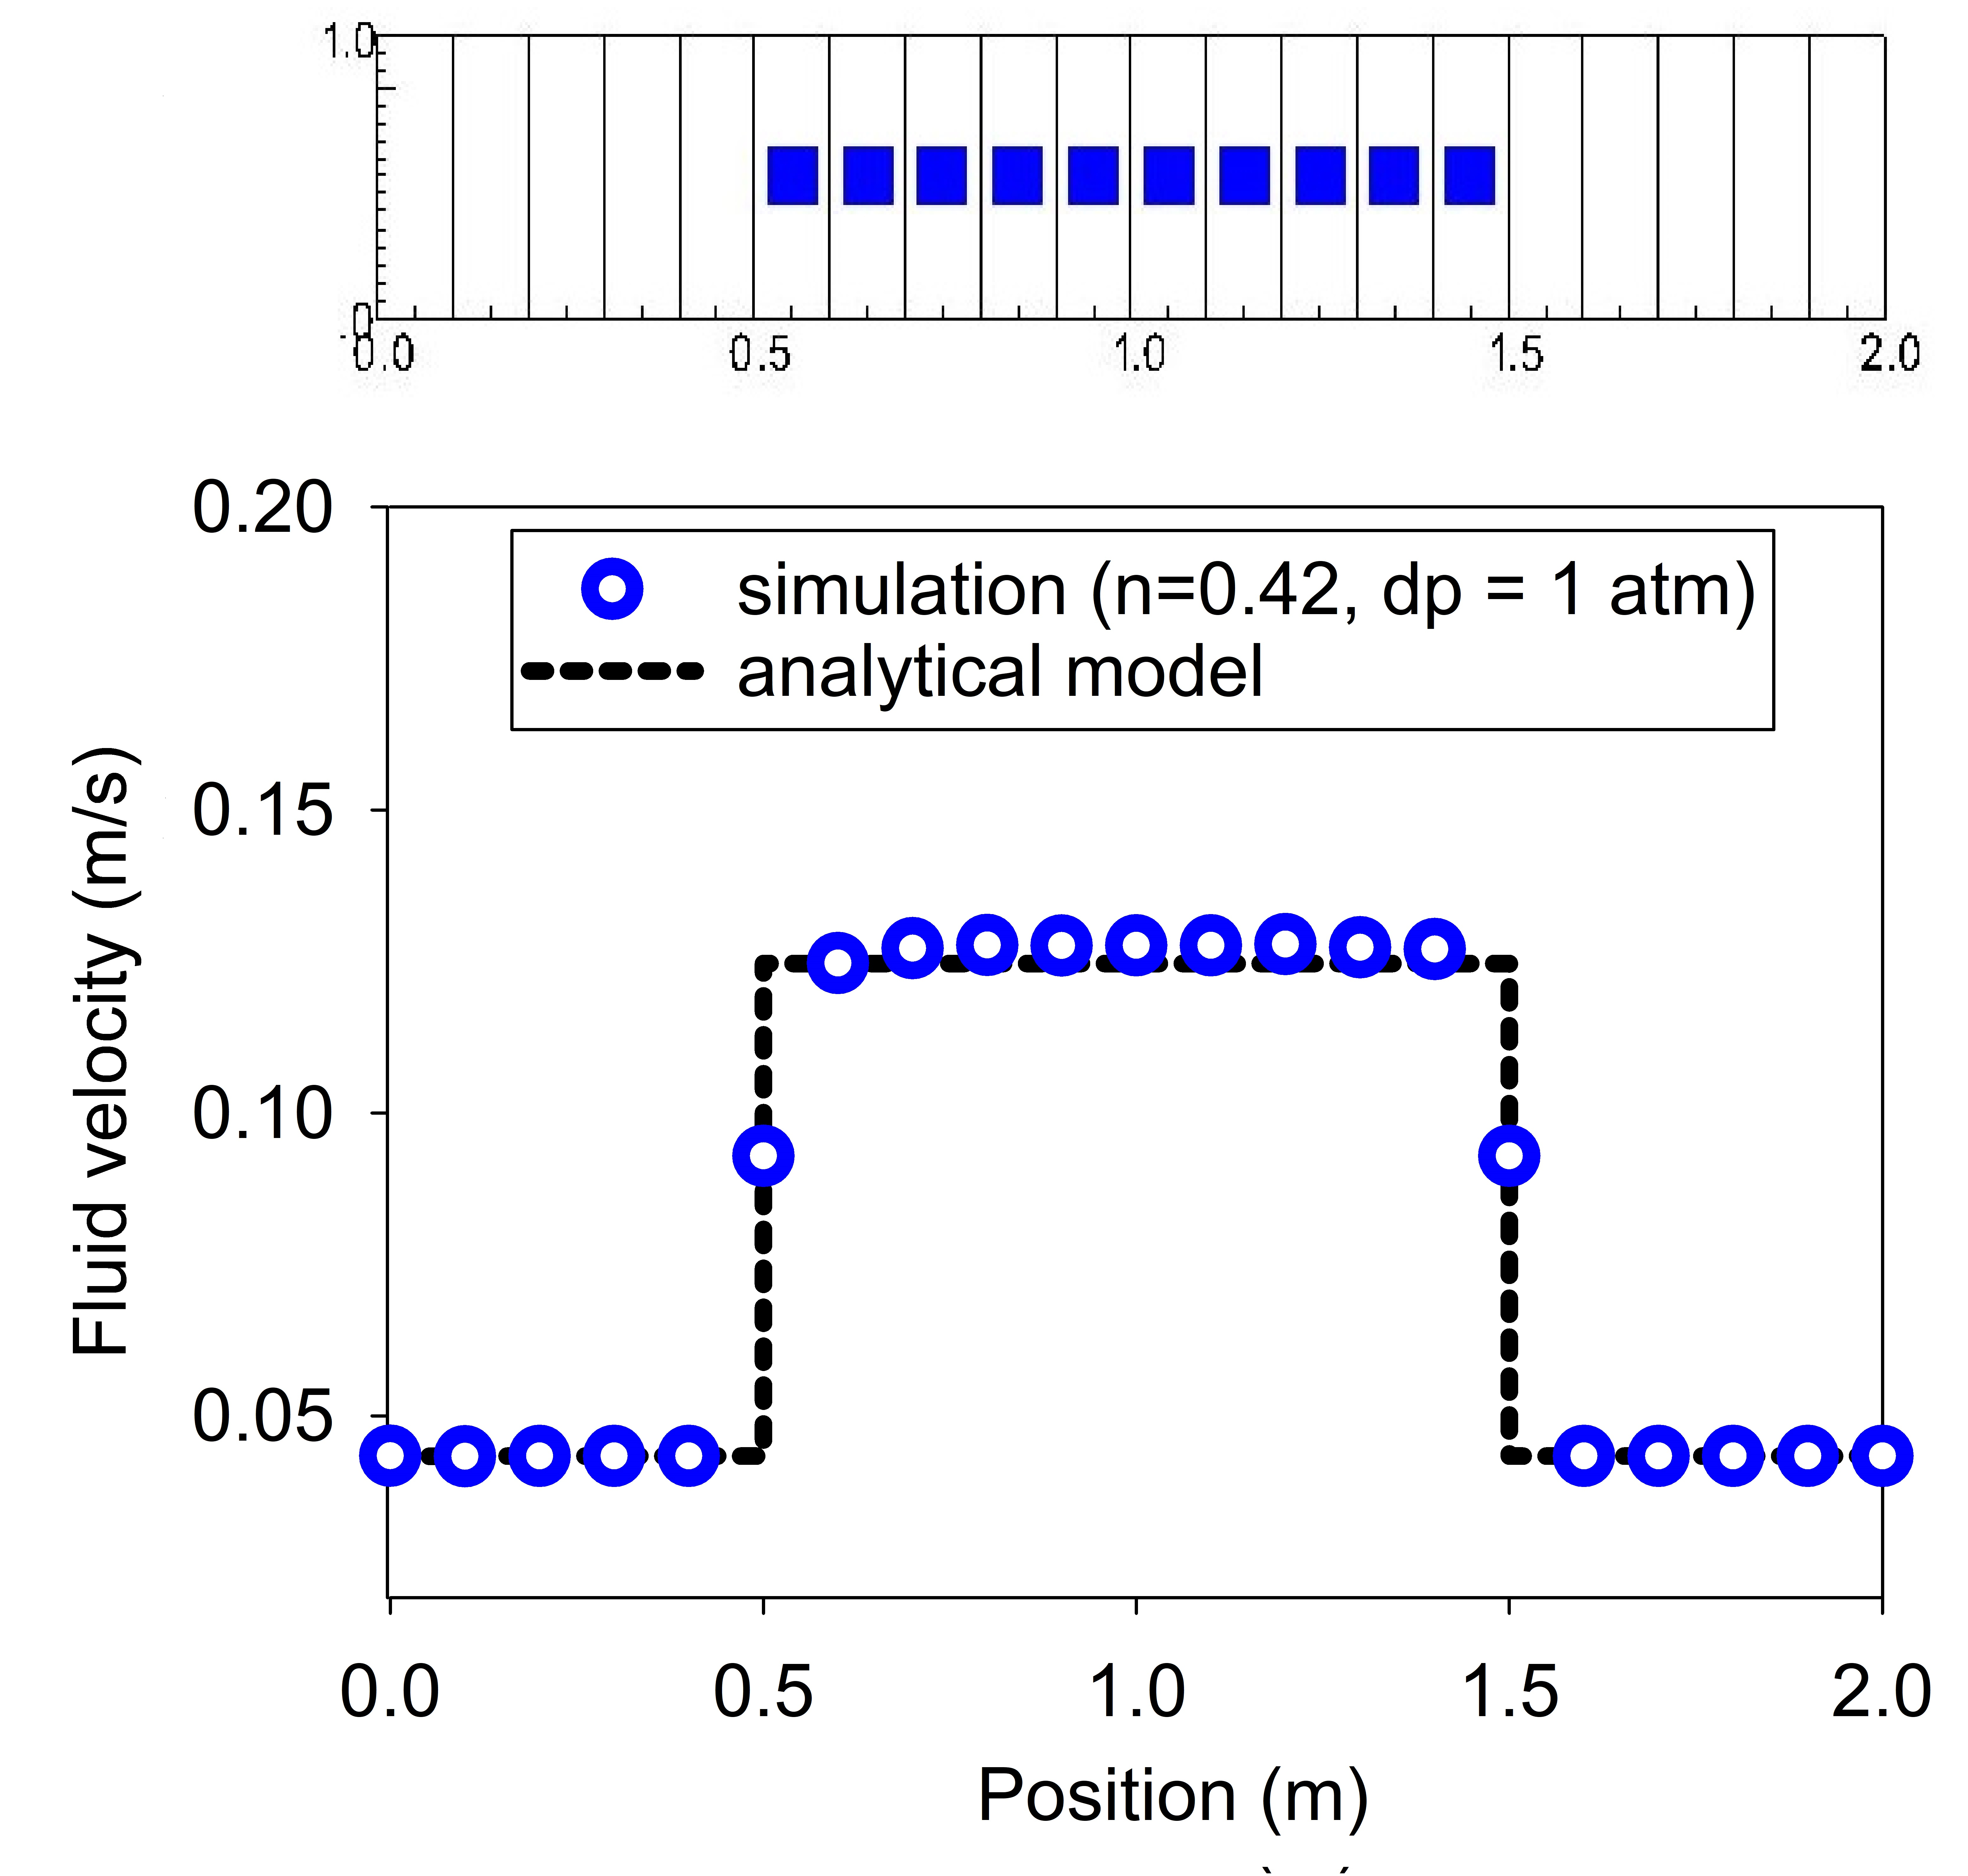
\includegraphics[width=\linewidth]{porousflow1.jpg}
\caption{Discretization of the model}
\label{fig:3c}
\end {subfigure}\hfill    
\begin{subfigure}[d]{0.5\linewidth}
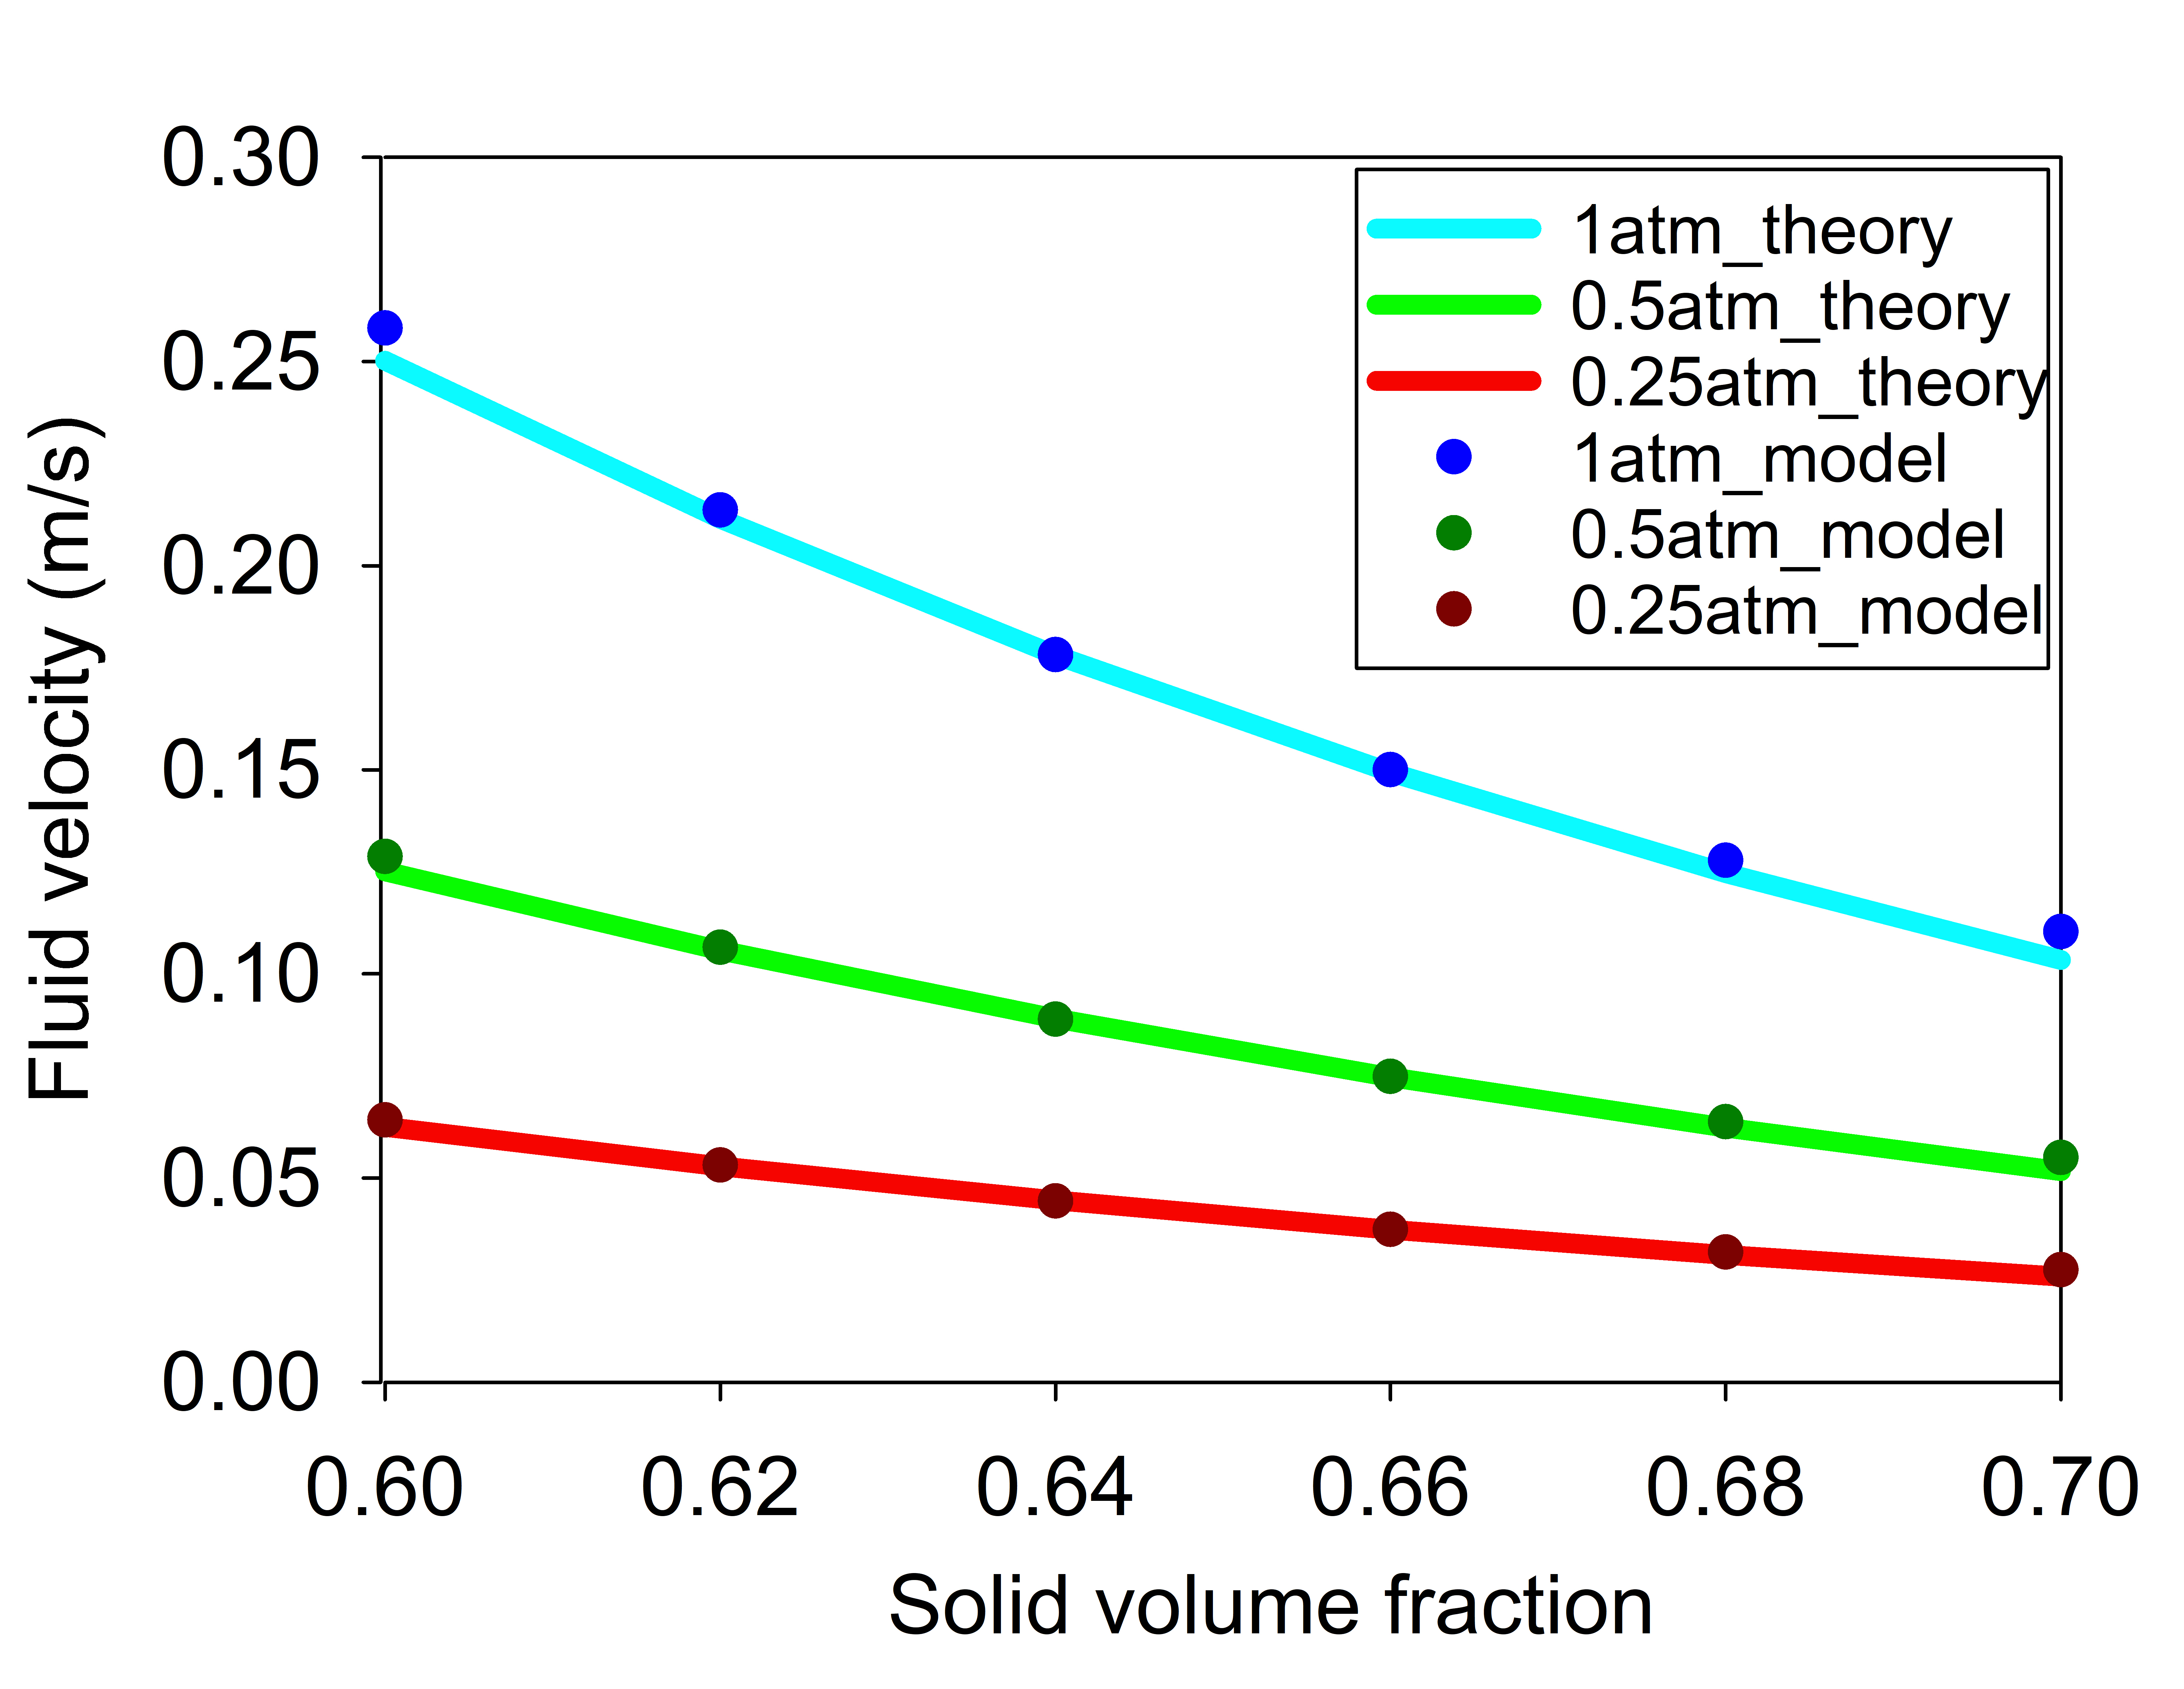
\includegraphics[width=\linewidth]{porousflow.jpg}
\caption{Comparison between analytical model and simulation}
\label{fig:3d}
\end {subfigure}
\caption{Numerical results of the fluid flow through isothermal porous media}
\label{fig:porousflow}
\end {figure}
%
%
Fluid flow through porous media is important in many engineering disciplines, like predicting water flow in soil. Fluid flow velocity in one dimension can be calculated from the porous media's hydraulic conductivity $K$ as:\\
%
%
\begin{equation}
  {U}_f   = K \frac{\Delta p_f}{L}
\end {equation}
%
%
If the Carman-Kozeny formula is adopted $F = 10\phi_s/(1-\phi_s)^2$, the hydraulic conductivity will be expressed as  $K = D_p^2 (1-\phi_s)^3 \rho_f  g / 180 \phi_s^2  \mu_f $. Then, the analytical formula of average velocity in one dimension through the porous media is:\\
%
%
\begin{equation}
  {U}_f  = \frac{1}{n} \frac{D_p^2 (1-\phi_s)^3}{180 \phi_s^2 \mu_f} \frac{\Delta p_f}{L}
\end {equation}

%
%
Our numerical model is validated by modeling fluid flow through a 1m long porous media. The porous media is modeled by elastic material with Young's modulus is 10 MPa, Poisson's ratio is 0.3, and density is 2650 kg/m3. The volume fraction of porous media $\phi_s$ is [0.6, 0.62, 0.66, 0.68, 0.7] and the average grain diameter $d$ is 1mm. The model is discretized in 20 finite element and the porous media in 10 finite element with 1 material point per element. The pressure gradient is applied with three different value [0.25, 0.5, 1] atm. Figure \ref{fig:porousflow} shows a good agreement of fluid flow prediction between the theory and the model.
%
%_______________________________
\subsection{\textsf{Isothermal consolidation}}
%
%
\begin{figure}[h]
\center
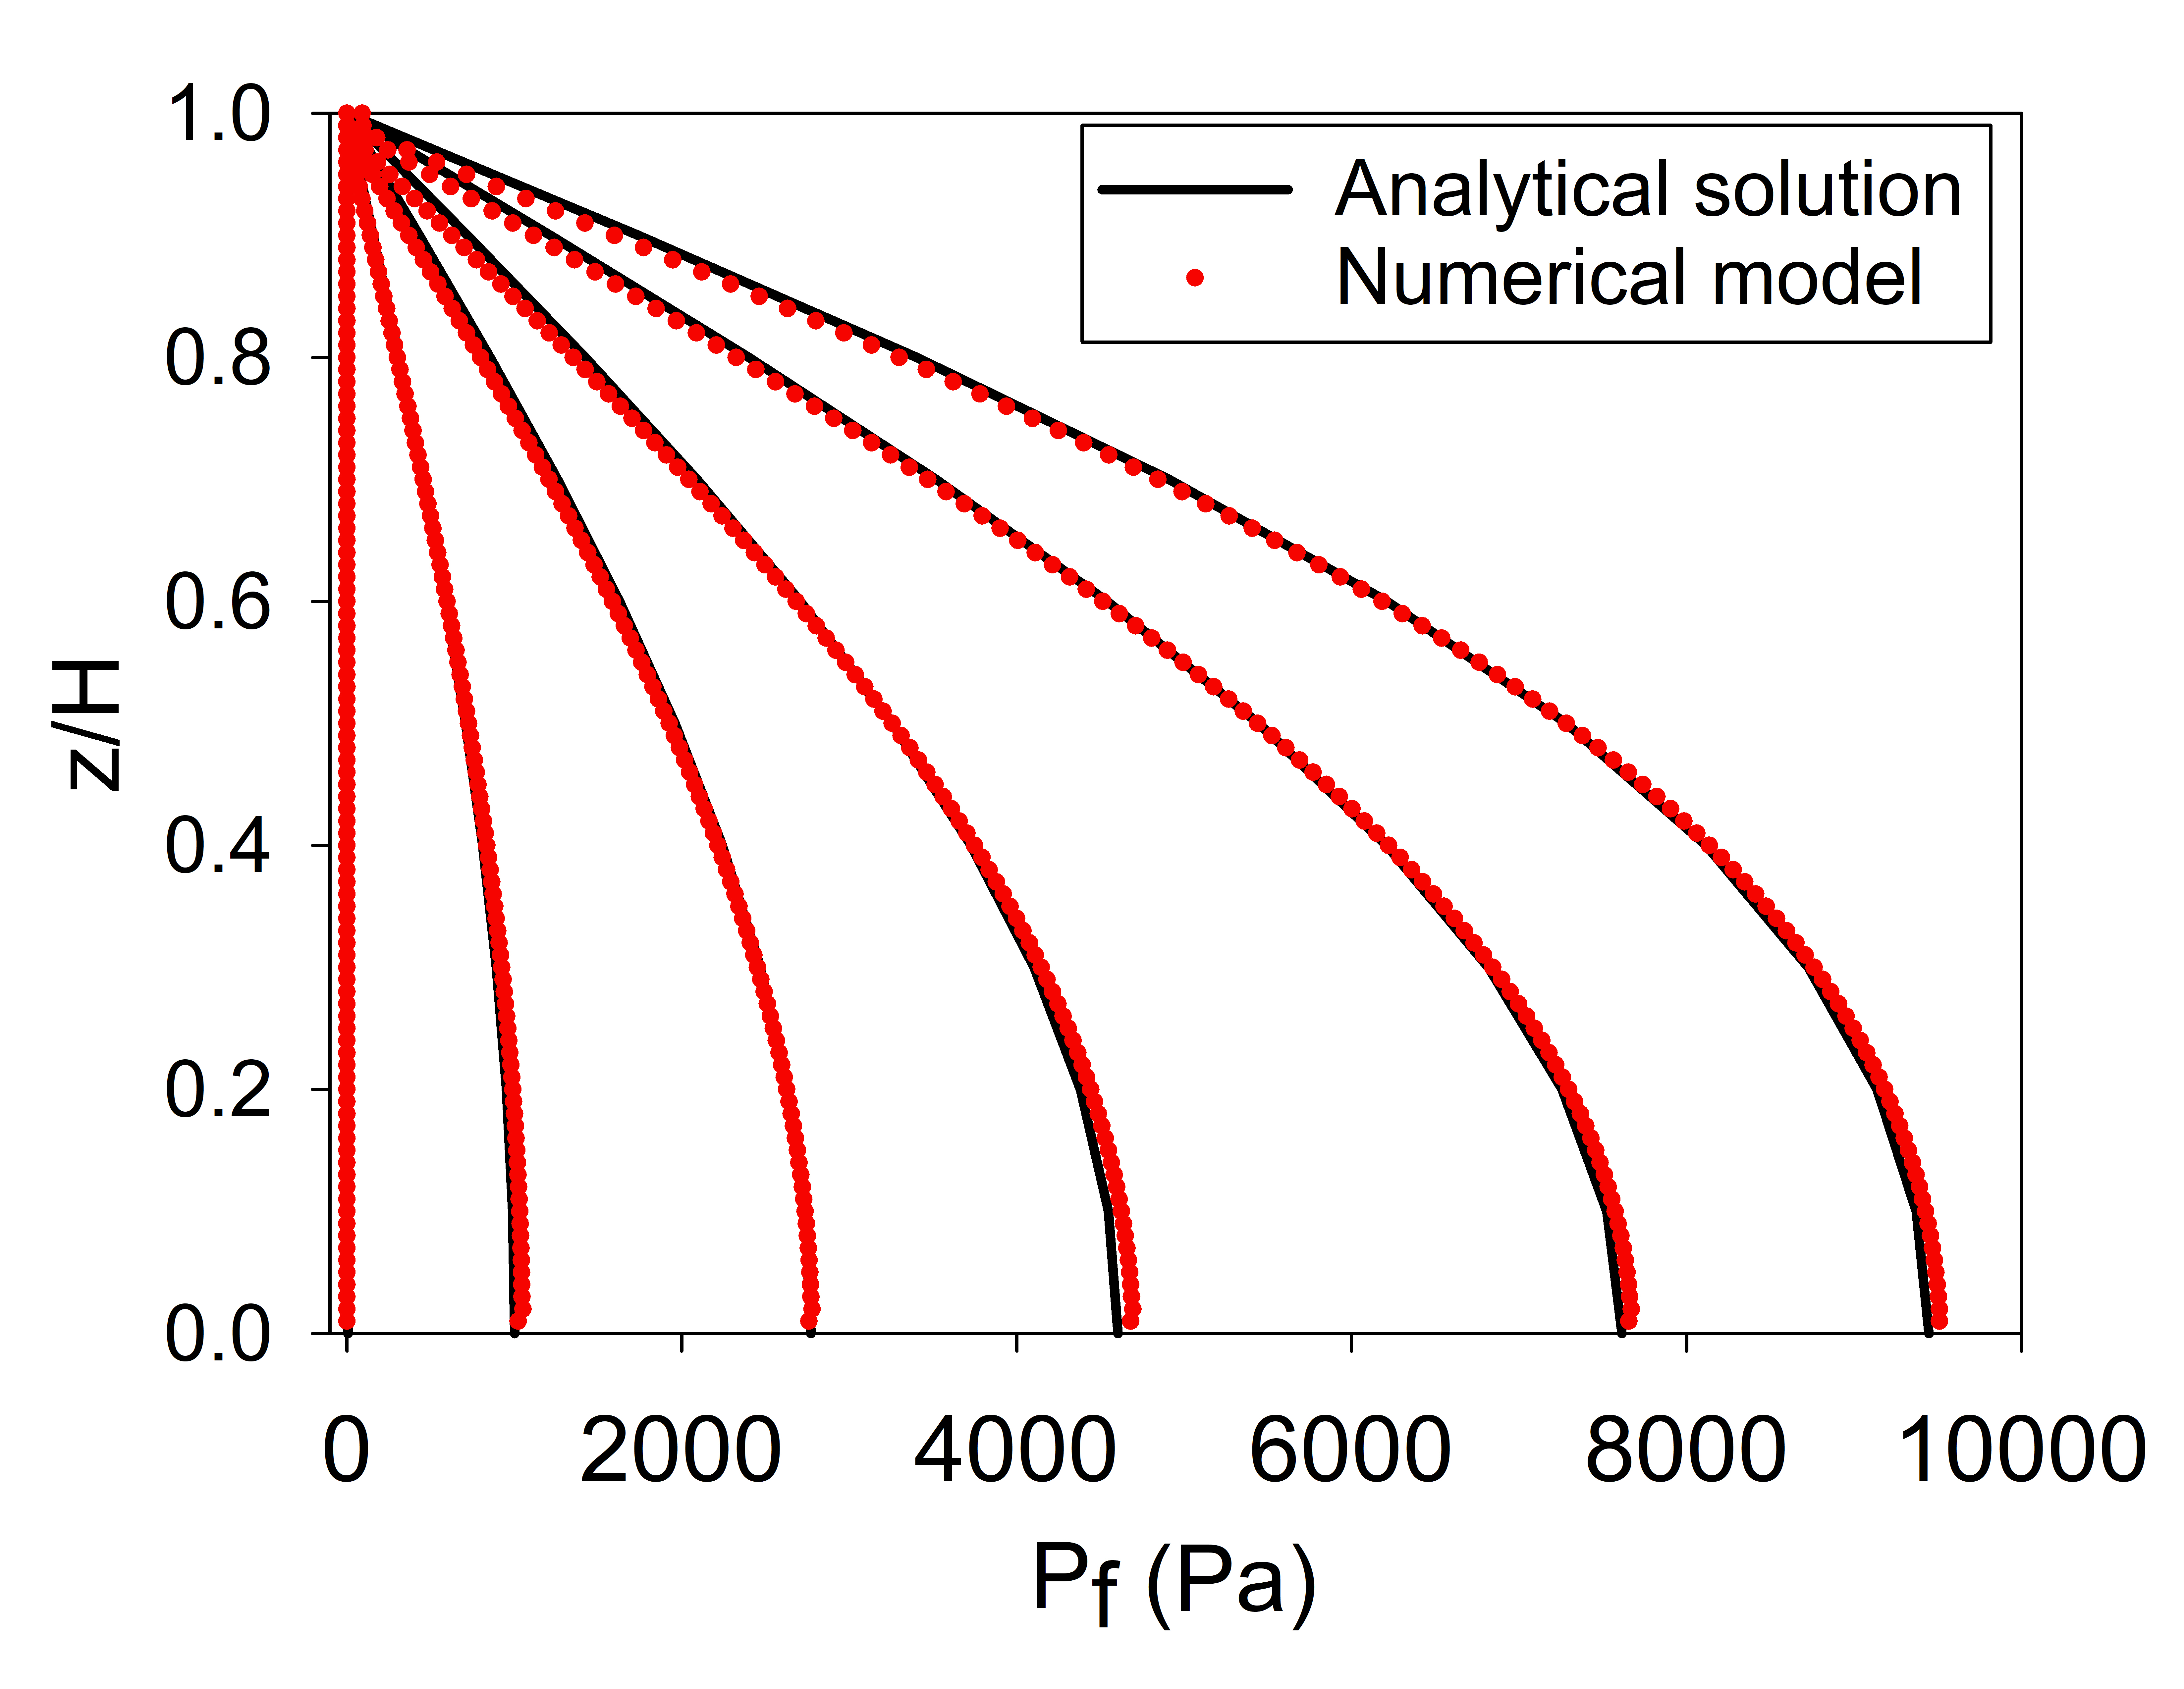
\includegraphics[scale=.3]{consolidation.jpg}
\caption{Compasion between analytical solution and numerical solution}
\label{fig:consolidation}
\end {figure}
%
%
A common benchmark for a fully saturated porous media is the simulation of one-dimensional consolidation. Using the Carman-Kozeny formula, the time-dependent pressure can be calculated as:
%
%
\begin{equation}
  p_f  = \sum_{m=1}^{\infty} \frac{2F_{ext}}{M} \sin (\frac{Mz}{H}) e^{-M^2T_V} \textrm{    with    }   M = \frac{\pi}{2} (2m+1)
\end {equation}
%
%
where the consolidation rate $T_v =C_vt/H^2$, the consolidation coefficient $C_v = E_v n^3 d^2/(180(1-n)^2\mu) $ and the Oedometer modulus $E_v = E(1-\upsilon)/(1+\upsilon)/(1-2\upsilon)$.
Our numerical model is validated by modeling the consolidation of a 1m column. The porous media is modeled by elastic material with Young's modulus is 10 MPa, Poisson's ratio is 0.3, and density is 2650 kg/m3. The volume fraction of porous media $\phi_s$ is 0.7 which is equivalent to the porosity of 0.3 and the average grain diameter $d$ is 1mm. The model is discretized in 100 finite element with 1 material point per element. The external pressure applies to the top of the column is 10 kPa. Figure \ref{fig:consolidation} shows a good agreement of fluid flow prediction between the theory and the model.
%_______________________________
\subsection{\textsf{Thermal induced cavity flow}}
%
%
\begin{figure}
\center
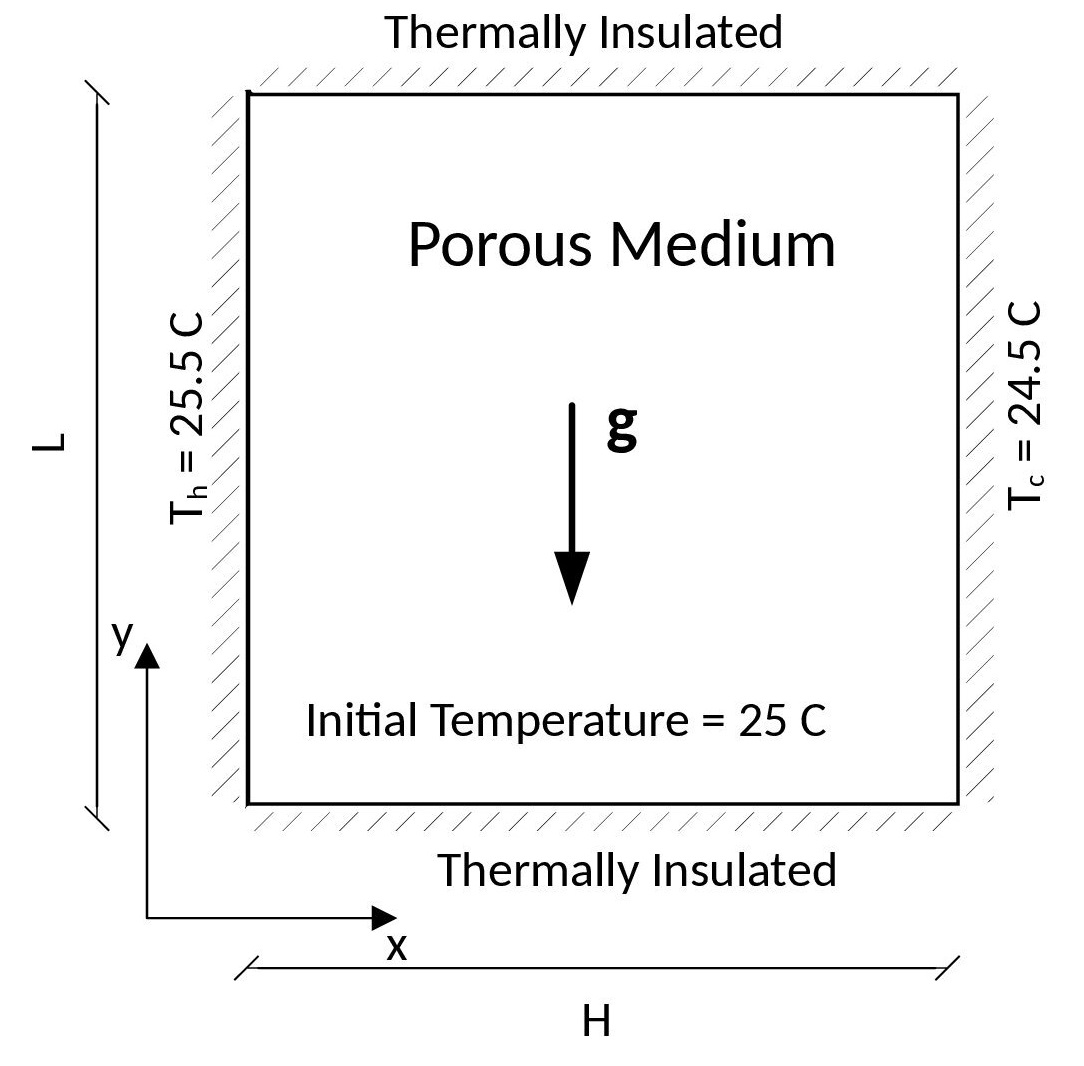
\includegraphics[scale=.5]{box_thermal.jpg}
\caption{Model schematic  \cite{Ali}}
\label{fig:thermalModel}
\end {figure}
%
%
\begin{figure}
\center
%add desired spacing between images, e. g. ~, \quad, \qquad, \hfill etc. 
%(or a blank line to force the subfigure onto a new line)
\begin{subfigure}[c]{0.5\linewidth}
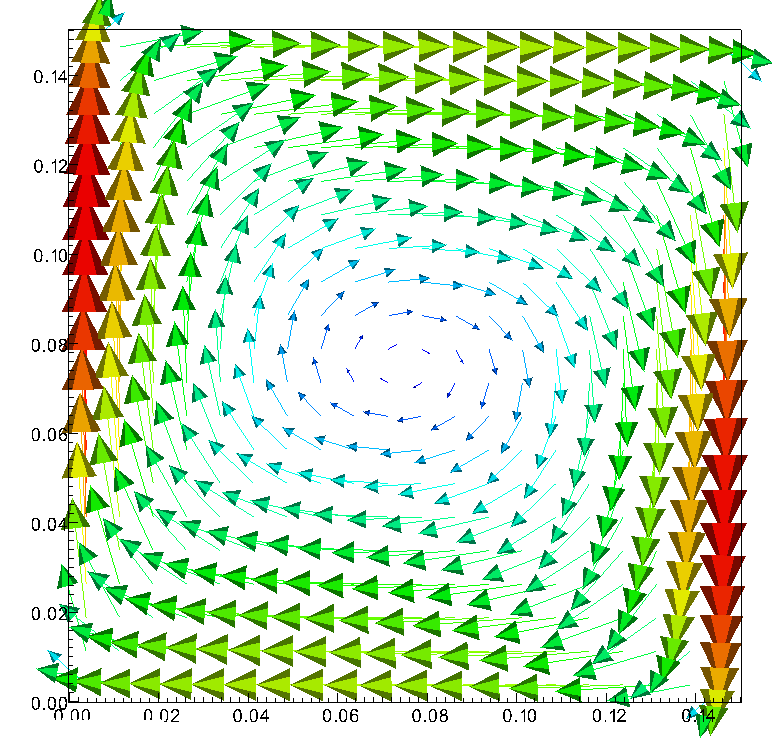
\includegraphics[width=\linewidth]{thermal.png}
\caption{MPMICE model}
\end {subfigure}\hfill    
\begin{subfigure}[d]{0.5\linewidth}
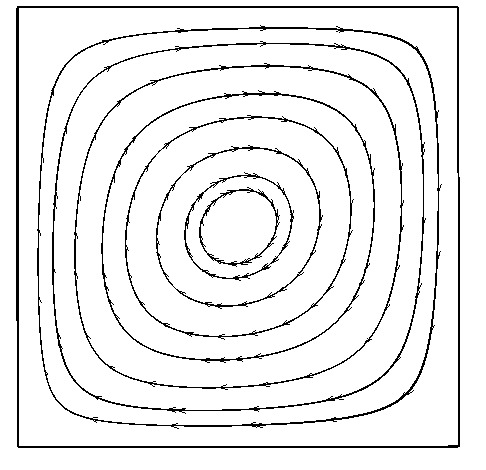
\includegraphics[width=\linewidth]{velocity_thermal-1.jpg}
\caption{FEM model \cite{Ali}}
\end {subfigure}
\caption{Comparison between MPMICE model and FEM model}
\label{fig:thermal}
\end {figure}
%
%
Another benchmark is the thermal induced cavity flow in porous media. Temperature and velocity distributions are calculated for a square non-deformable saturated porous media The top and bottom walls are insulated, and the left and right walls are at fixed temperature gradient of 1 degree. The fluid motion at stead state are cavity flow due to the temperature induced density variation. The numerical is validated by comparing with the numerical solution of the finite element method. The porous media is modeled by non deformable material, and density is 2500 kg/m3. The specific heat capacity of the water and porous skeleton are 4181 J/kg.K and 835 J/kg.K respectively. The thermal conductivity of the water and porous skeleton are 0.598 W/m.K and 0.4 W/m.K. The volume fraction of porous media $\phi_s$ is 0.6 which is equivalent to the porosity of 0.4 and the average grain diameter $d$ is 1mm. The model is discretized in 20 x 20 finite element with 4 material point per element. Figure \ref{fig:thermal} shows a good agreement of numerical results of the model compared with the numerical solution of the finite element method.
%_______________________________
\subsection{\textsf{Underwater debris flow}}
%
%
\begin{figure}[h]
\center
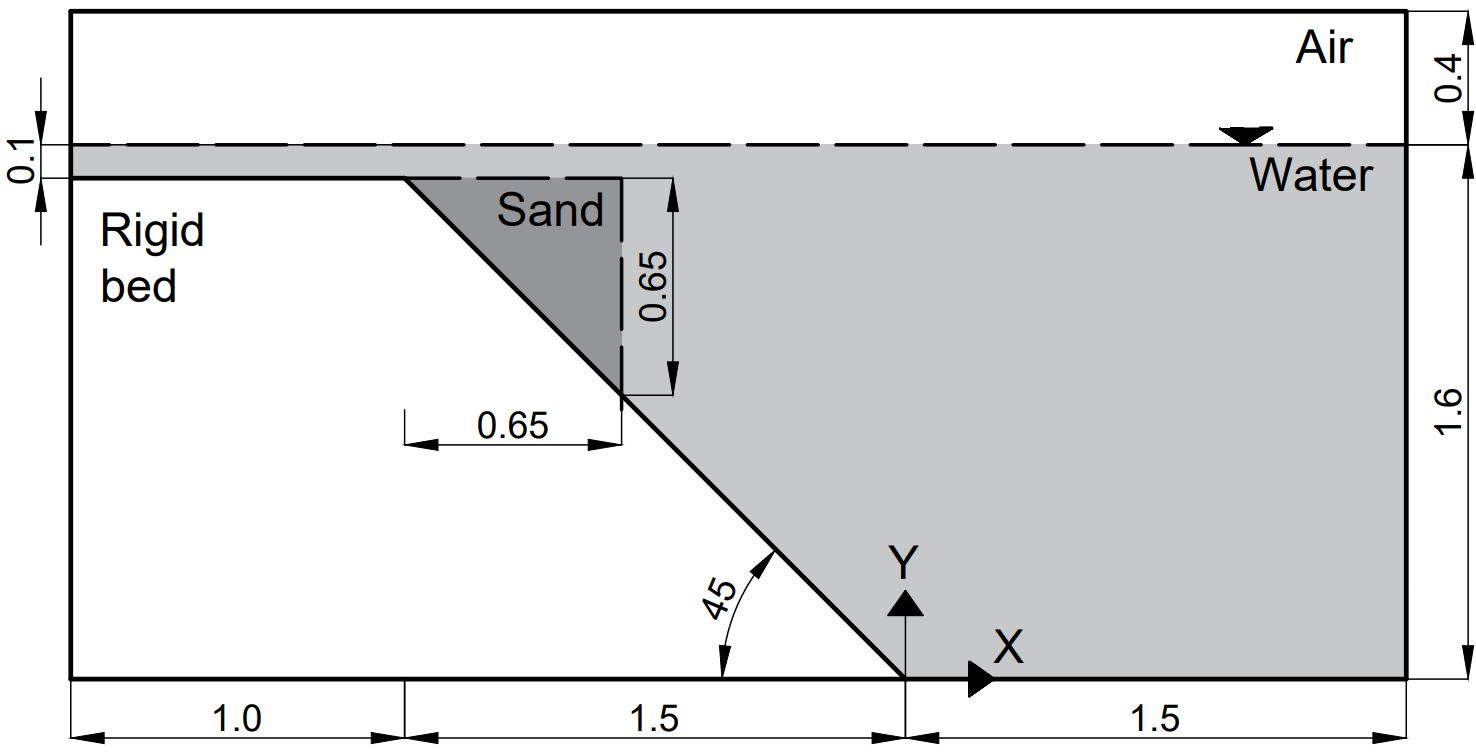
\includegraphics[scale=.3]{SandBoxscheme.jpg}
\caption{Model schematic}
\label{fig:SandBoxModel}
\end {figure}
%
%

The numerical example is validated using the experimental work of Rzadkiewicz et al. on submarine debris flow \cite{Rzadkiewicz}. In their experiment, sand within a triangular box is released and slides along a rigid bed inclined at 45 degrees under water (see Figure \ref{fig:SandBoxModel}). The material properties in the numerical model are selected based on the experiment by Rzadkiewicz et al. \cite{Rzadkiewicz}. The sand is characterized by a saturated density of 1985 $kg/m^3$ and a friction angle of 10 degrees. The effect of Young's modulus on debris flow run-out is negligible due to the extreme deformation of the debris, so a Young's modulus of 50 MPa with a Poisson's ratio of 0.25 is chosen. The rigid bed, being much stiffer, has bulk modulus and shear modulus values of $117E^7$ Pa and $43.8E^7$ Pa, respectively. The numerical parameters used in this example are presented in Table \ref{table2}.\\
The boundary conditions imposed in the numerical model are as follows: on all boundary faces, the velocity is set to zero (U = 0 m/s) and the temperature is set to 5 degrees Celsius (T = 5°C). At the top boundary, the pressure has a Neumann boundary condition of dp/dx = 0 kPa, and the density has a Neumann boundary condition of d$\rho$/dx = 0 $kg/m^3$. The background mesh consists of 700 x 400 cells, resulting in a total of 280,000 cells. Each cell in the debris flow and rigid bed contains 2 x 2 material points.\\
Figure \ref{saturatedflowb} illustrates snapshots of the underwater debris flow sliding, demonstrating that the model captures the typical hydroplaning mechanism of the debris flow. Hydroplaning refers to the lifting of the debris flow, causing it to lose contact with the bottom layer. The elevation of the free surface at 0.4s and 0.8s is compared between our proposed method and other methods in Figure \ref{watersurface}. Our computed results align well with the experimental results \cite{Zhang2019}.\\
Unlike other computational models that rely on total stress analysis \cite{Tran2019, Capone2010, Zhang2019, Dey2016}, our proposed model utilizes effective stress analysis, enabling the analysis of water pressure and temperature within the debris flow. Additionally, we investigate the differences between underwater debris flow and saturated debris flow in terms of their interaction with obstacles. Figure \ref{saturatedflow} presents snapshots of simulations of both underwater and saturated debris flow. The saturated debris flow (Figure \ref{saturatedflowa}) exhibits behavior similar to frictional flow, where grains have contact forces with each other. Conversely, the underwater debris flow (Figure \ref{saturatedflowb}) behaves like turbulent flow, with grains being separated from each other and exhibiting no contact forces (as reflected by the near-zero effective stress in the turbulence domain).
%
%
%\begin{figure}
%\center
%add desired spacing between images, e. g. ~, \quad, \qquad, \hfill etc. 
%(or a blank line to force the subfigure onto a new line)
%\begin{subfigure}[c]{0.5\linewidth}
%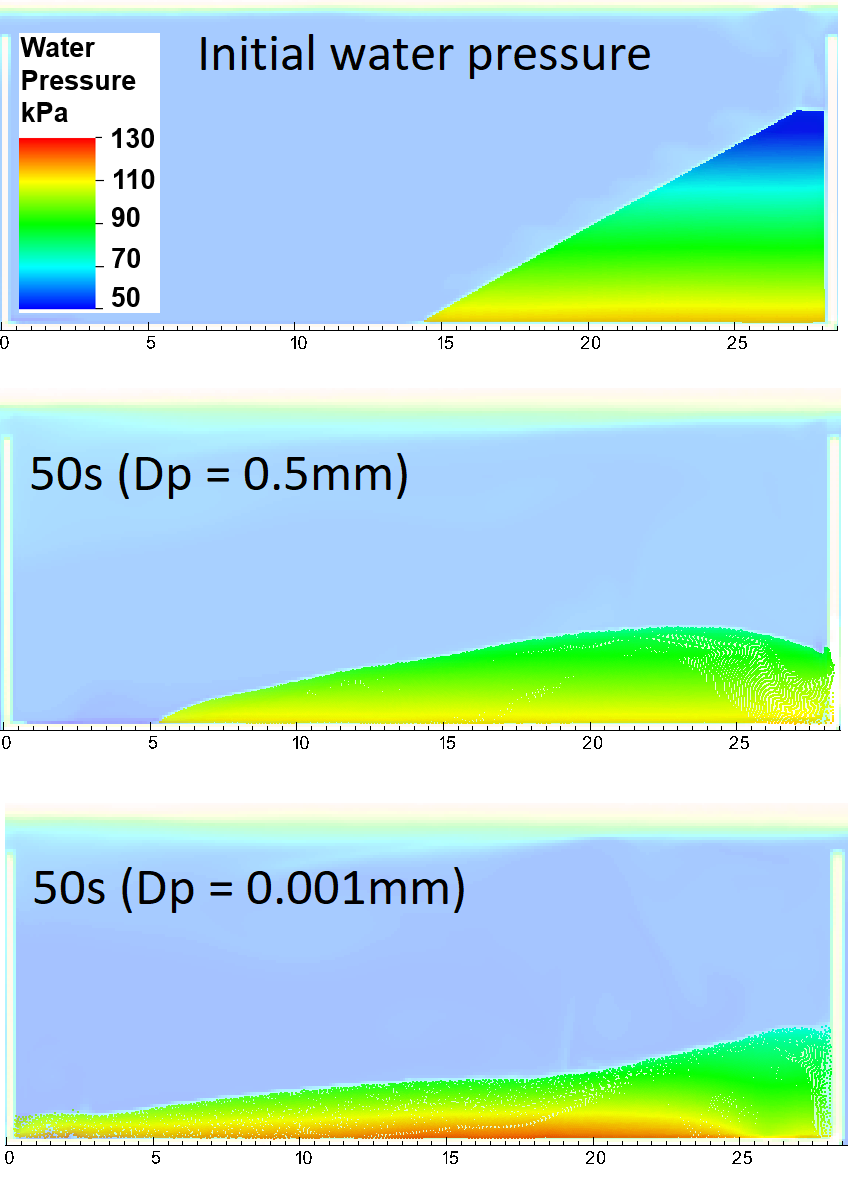
\includegraphics[width=\linewidth]{1.jpg}
%\caption{0.4 seconds}
%\label{0.4s}
%\end {subfigure}\hfill    
%\begin{subfigure}[d]{0.5\linewidth}
%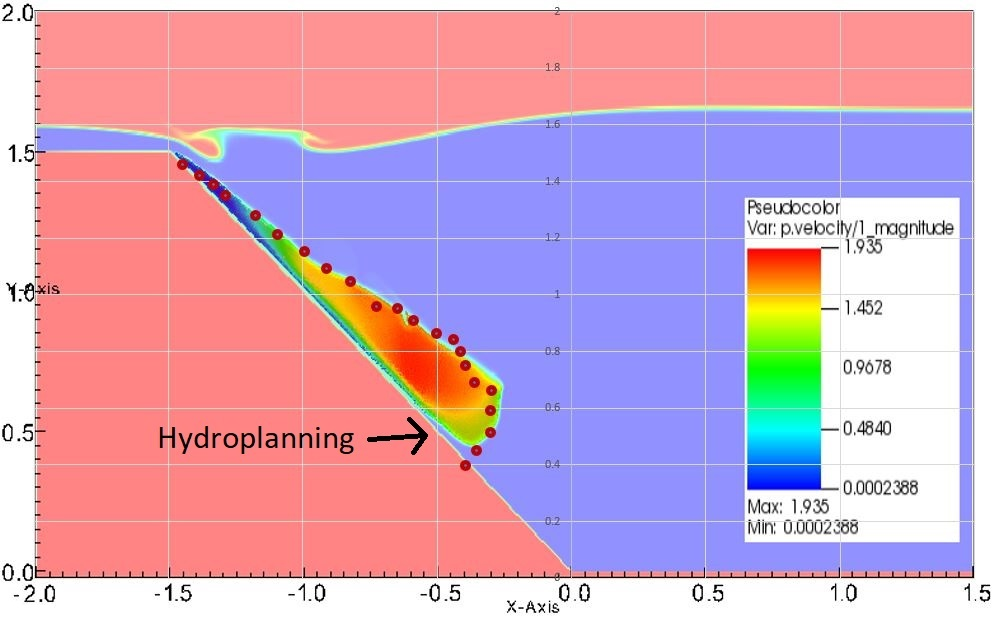
\includegraphics[width=\linewidth]{2.jpg}
%\caption{0.8 seconds}
%\label{0.8s}
%\end {subfigure}
%\caption{Simulation of underwater debris flow}
%\label{fig:debris}
%\end {figure}
%
%
\begin{table}[h]
\center
\begin{tabular}{|c|c|c|c|c|c|c|}
\hline
\textbf{Materials}                                                 & \textbf{\begin{tabular}[c]{@{}c@{}}Bulk \\ modul\\ (Pa)\end {tabular}} & \textbf{\begin{tabular}[c]{@{}c@{}}Shear \\ modul\\ (Pa)\end {tabular}} & \textbf{\begin{tabular}[c]{@{}c@{}}Density\\ (kg/m3)\end {tabular}} & \textbf{\begin{tabular}[c]{@{}c@{}}Temp\\ (C)\end {tabular}} & \textbf{\begin{tabular}[c]{@{}c@{}}Dynamic \\ vicosity\\ (Pa s)\end {tabular}} & \textbf{\begin{tabular}[c]{@{}c@{}}Friction \\ angle\\ (degrees)\end {tabular}} \\ \hline
\begin{tabular}[c]{@{}c@{}}Water\\ (at surface)\end {tabular}       & 2.15e9                                                                  & -                                                                        & 999.8                                                              & 5                                                           & 855e-6                                                                        & -                                                                       \\ \hline
\begin{tabular}[c]{@{}c@{}}Air\\ (at top \\ boundary)\end {tabular} & -                                                                       & -                                                                        & 1.177                                                              & 5                                                           & 18.45e-6                                                                      & -                                                                       \\ \hline
\begin{tabular}[c]{@{}c@{}}Sand\\ (porous \\ media)\end {tabular}   & 8.33e6                                                                  & 20e6                                                                     & 1985                                                               & 5                                                           & -                                                                             & 10                                                                     \\ \hline
\begin{tabular}[c]{@{}c@{}}Rigid bed\\ (solid)\end {tabular}        & 117e7                                                                 & 43.8e7                                                                   & 8900                                                               & 5                                                           & -                                                                             & -                                                                       \\ \hline
\end {tabular}
\caption{Numerical parameters for the underwater submarine debris}
\label{table2}
\end {table}

%
%
\begin{figure}[H]
\center
%add desired spacing between images, e. g. ~, \quad, \qquad, \hfill etc. 
%(or a blank line to force the subfigure onto a new line)
\begin{subfigure}[c]{0.5\linewidth}
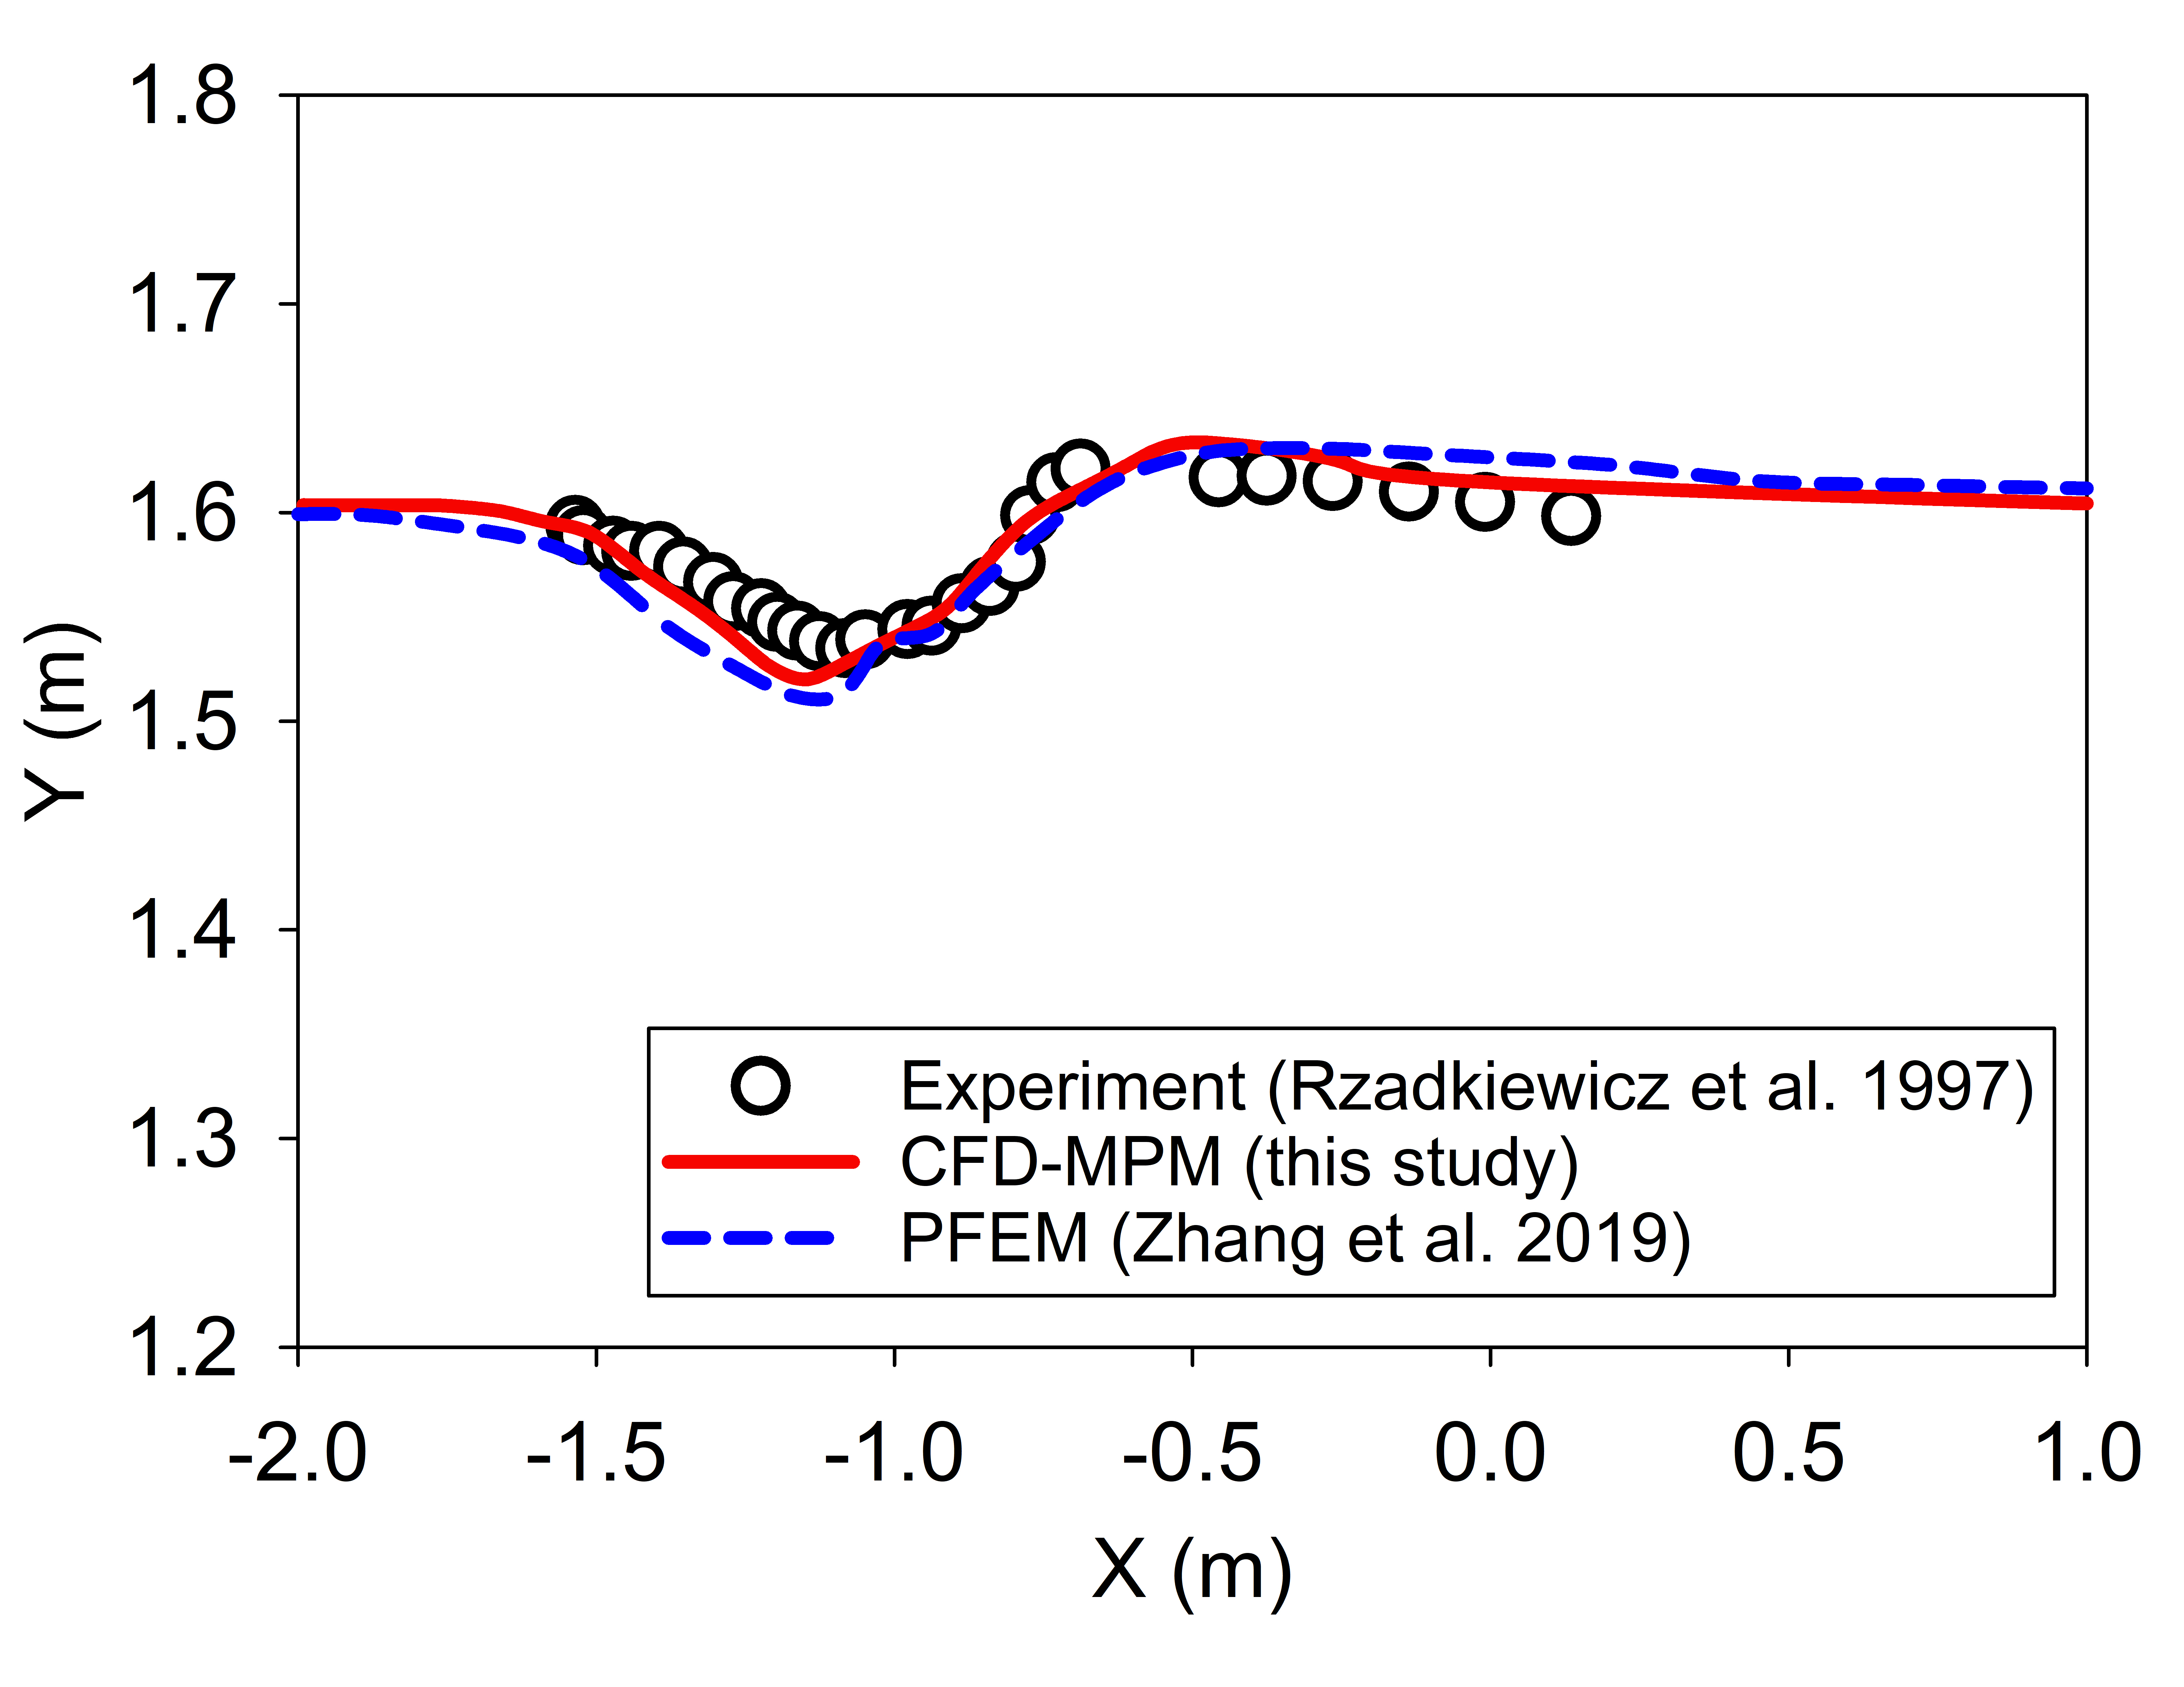
\includegraphics[width=\linewidth]{0.4swater.jpg}
\caption{0.4 seconds}
\label{0.4swater}
\end {subfigure}\hfill    
\begin{subfigure}[d]{0.5\linewidth}
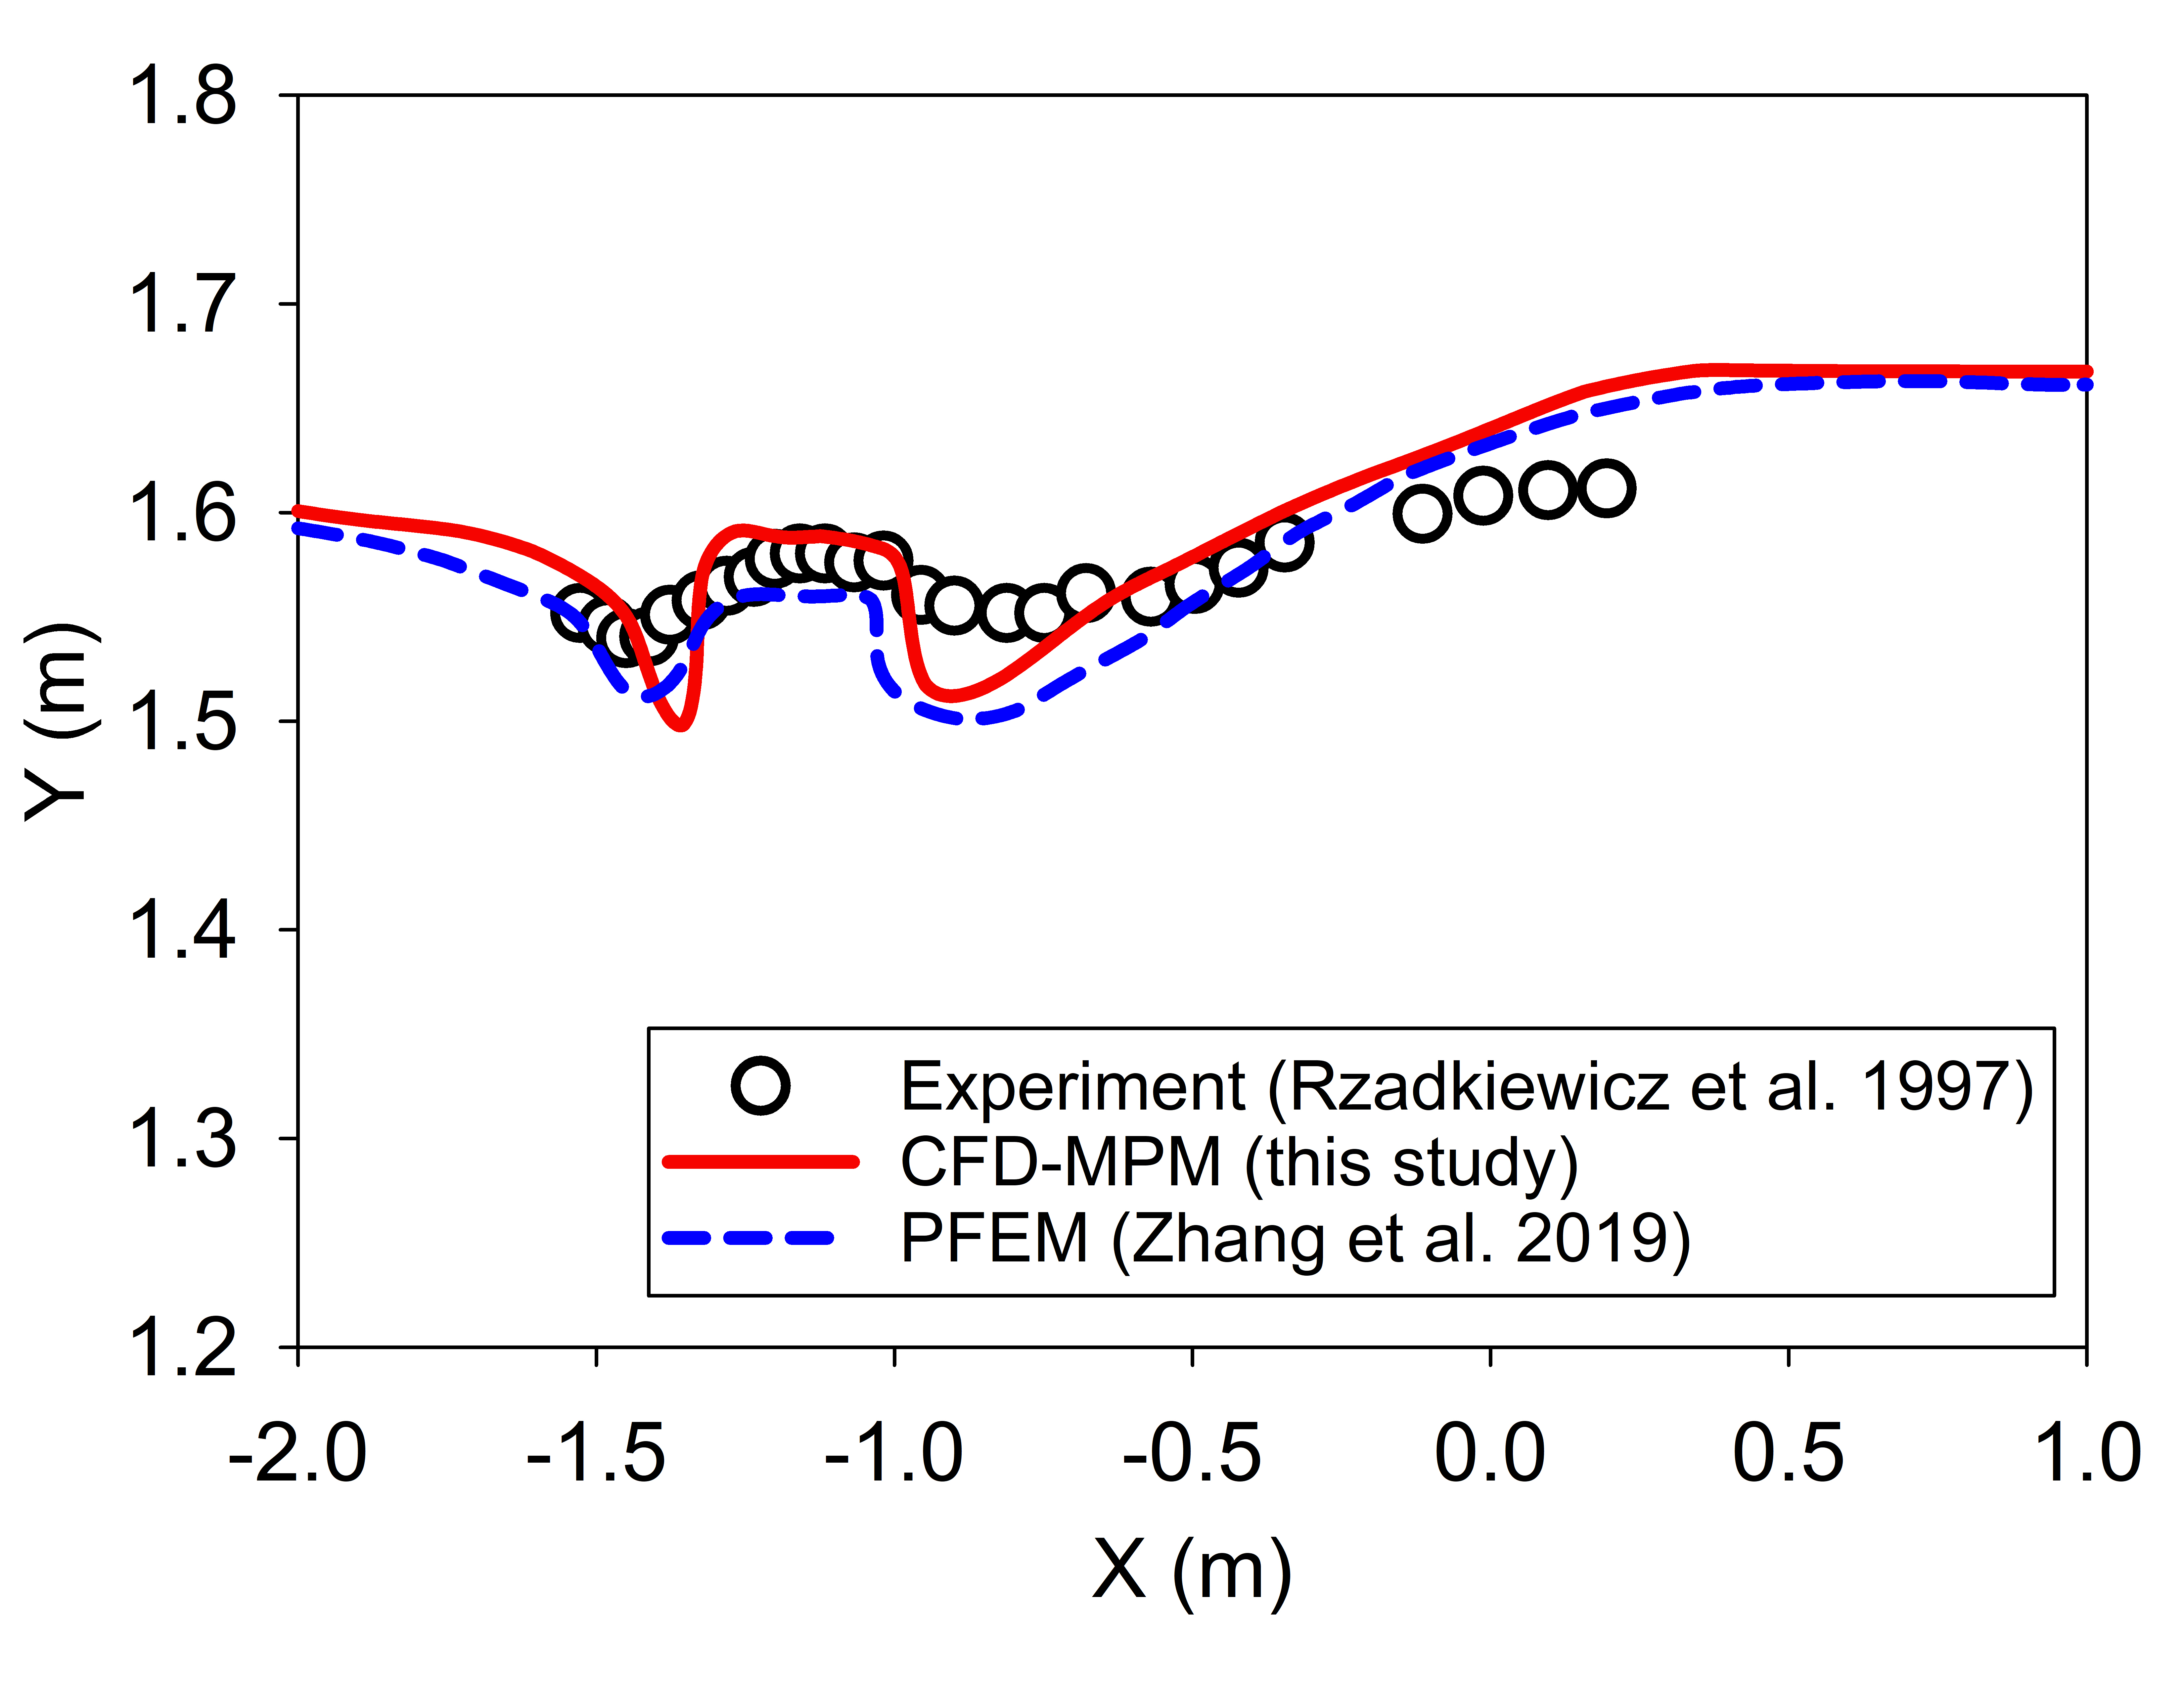
\includegraphics[width=\linewidth]{0.8swater.jpg}
\caption{0.8 seconds}
\label{0.8swater}
\end {subfigure}
\caption{Evolution of water level in the simulation of underwater debris flow}
\label{watersurface}
\end {figure}
%
%
%
%
\begin{figure}[]
\center
%add desired spacing between images, e. g. ~, \quad, \qquad, \hfill etc. 
%(or a blank line to force the subfigure onto a new line)
\begin{subfigure}[c]{0.5\linewidth}
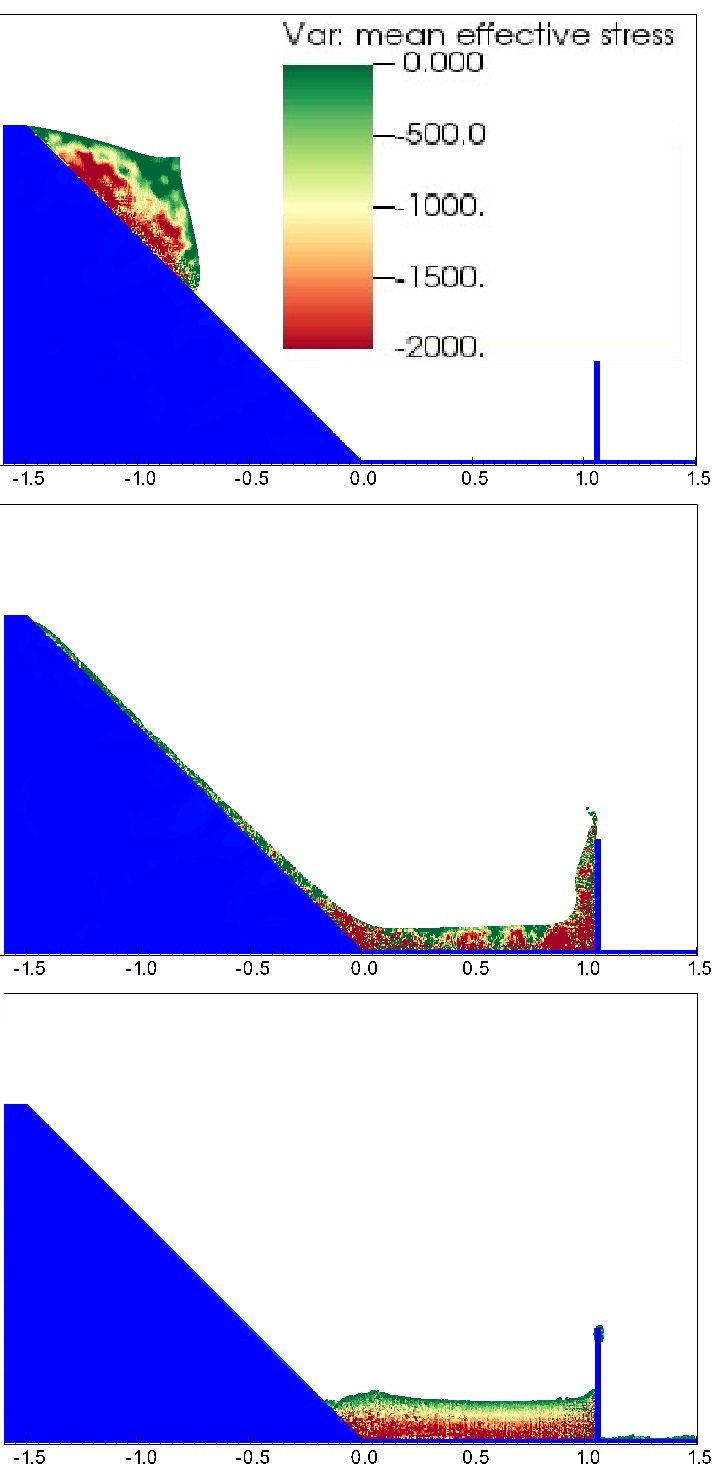
\includegraphics[width=\linewidth]{SHMPM.jpg}
\caption{saturated debris flow using MPM}
\label{saturatedflowa}
\end {subfigure}\hfill    
\begin{subfigure}[d]{0.5\linewidth}
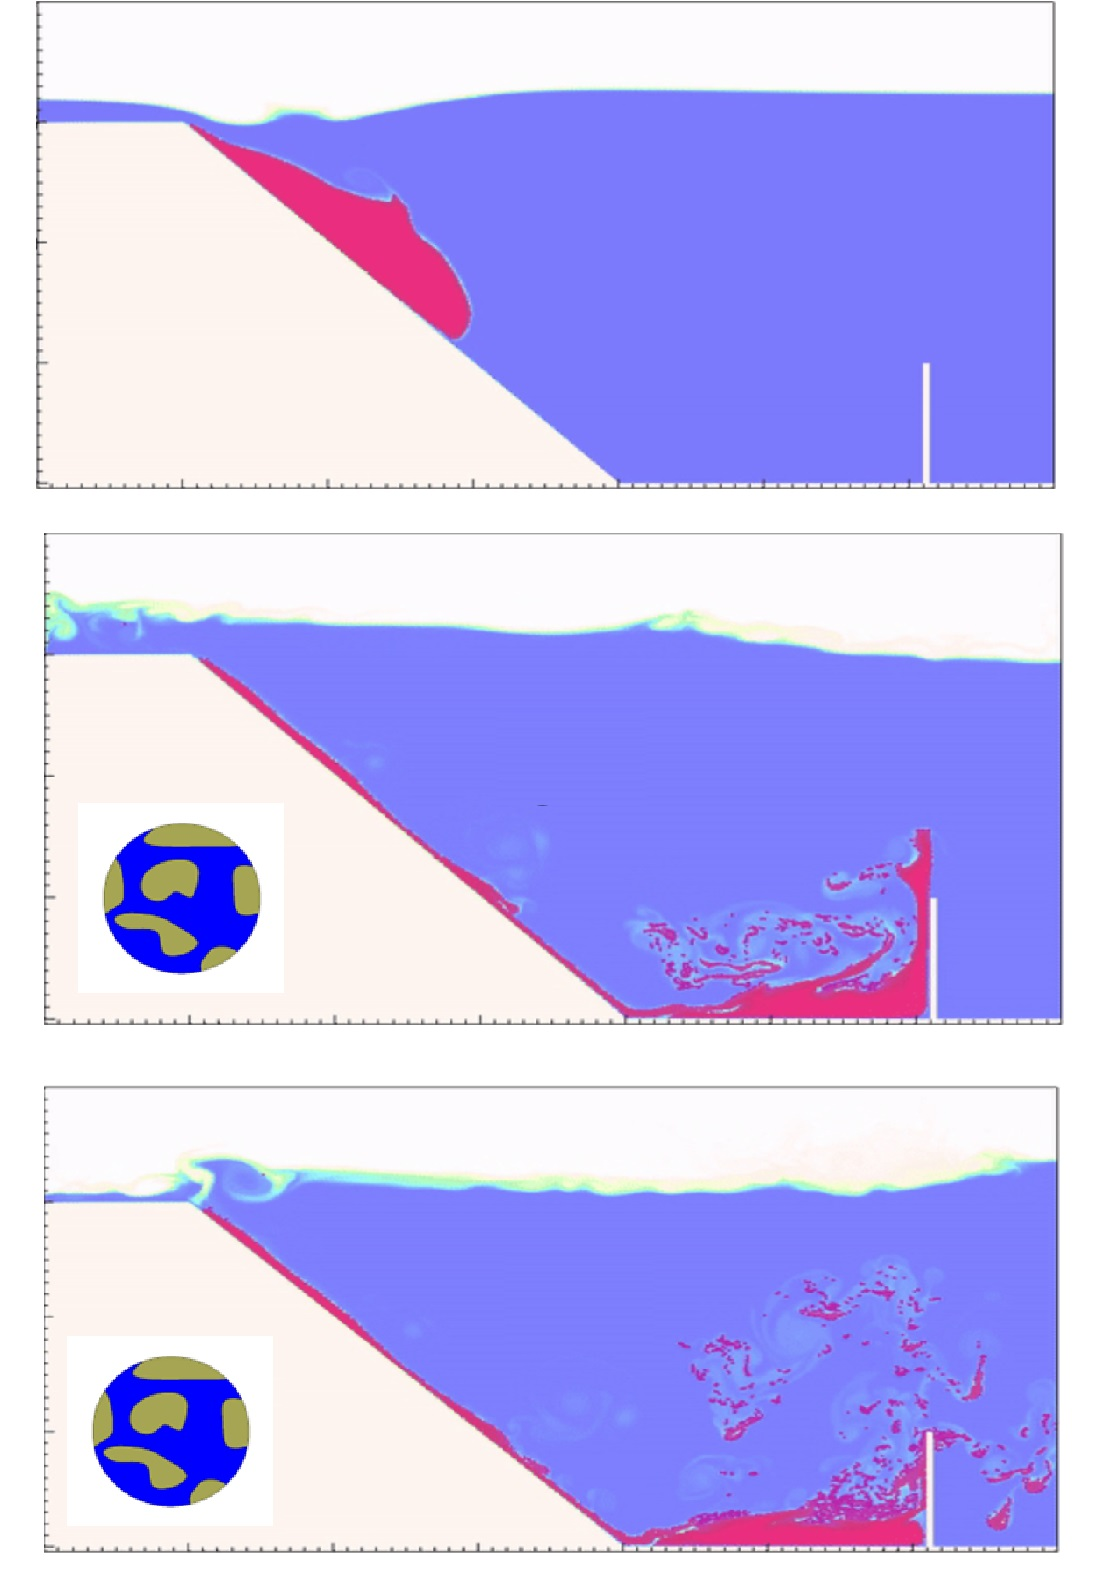
\includegraphics[width=\linewidth]{MPMICE_debris.jpg}
\caption{underwater debris flow using MPMICE}
\label{saturatedflowb}
\end {subfigure}
\caption{Simulation of Debris Flow: Mean Effective Stress Distribution (Green Color Indicates Near-Zero Effective Stress)}
\label{saturatedflow}
\end {figure}
%
%

%_______________________________
\subsection{\textsf{Validation of soil response to the seismic loading}}
%
%
\begin{figure}[H]
\center
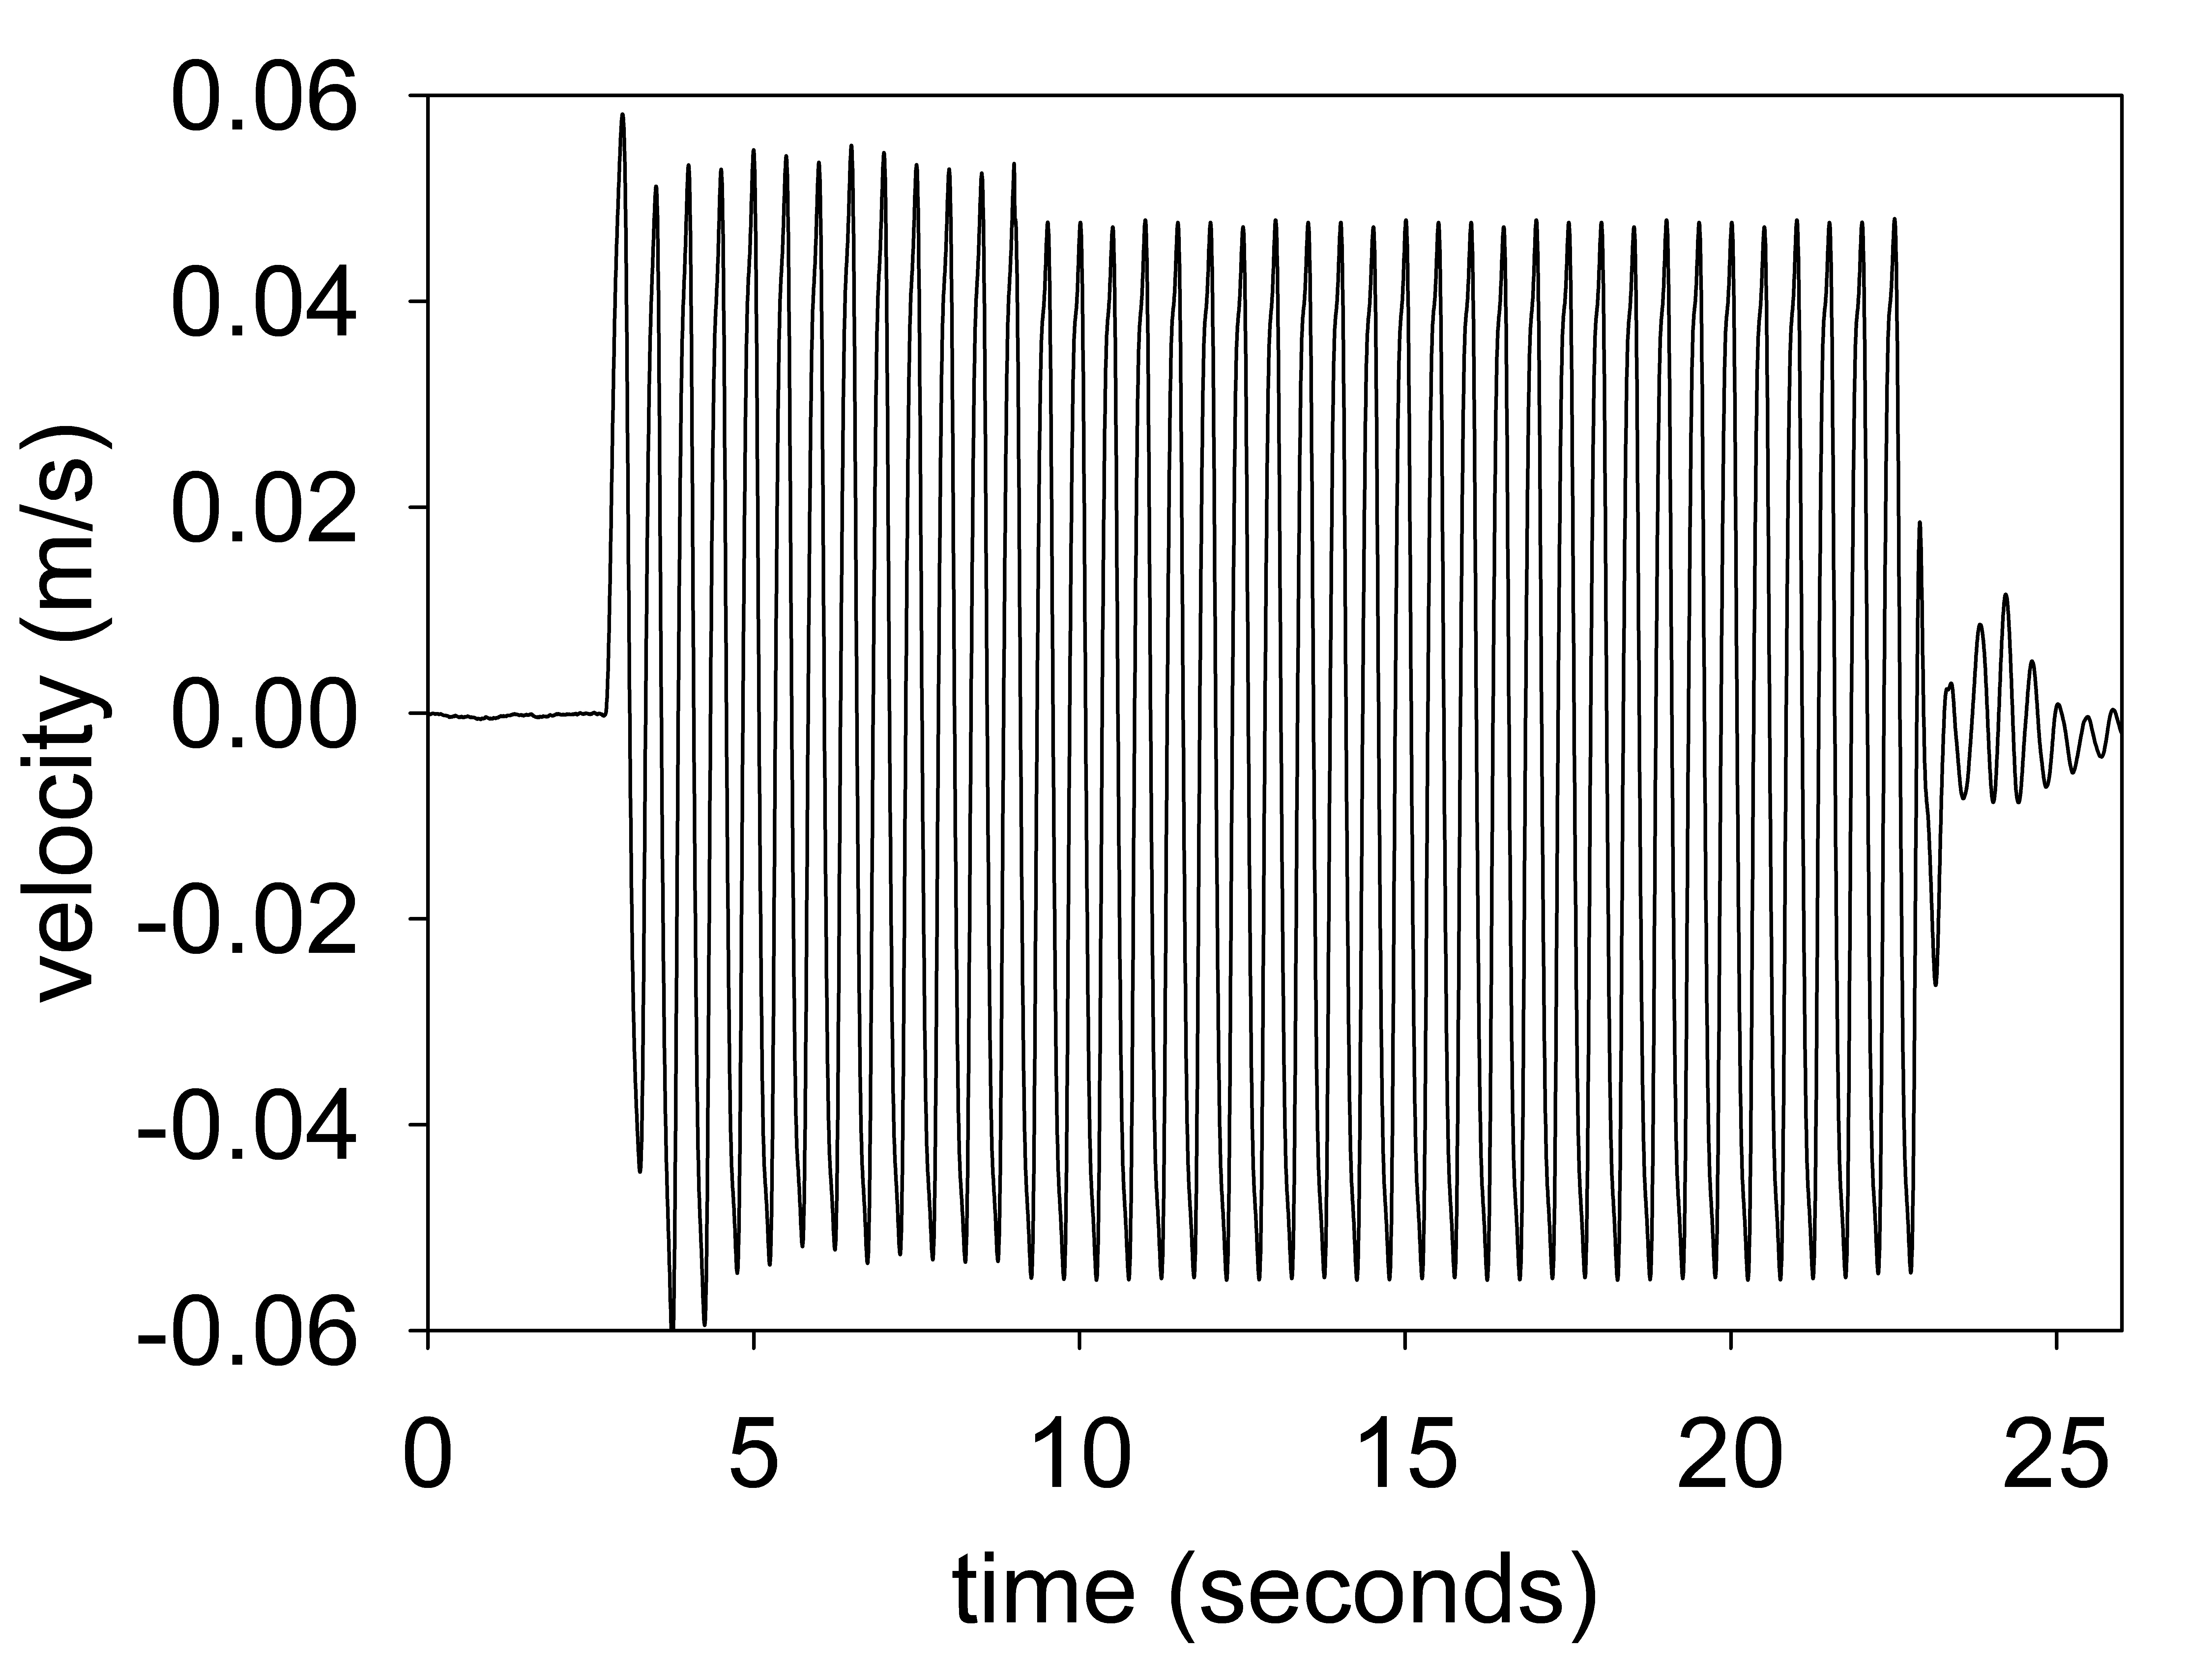
\includegraphics[scale=0.25]{vel.jpg}
\caption{Seismic loading}
\label{fig:vel_profile}
\end {figure}
%
%
\begin{figure}[H]
\center
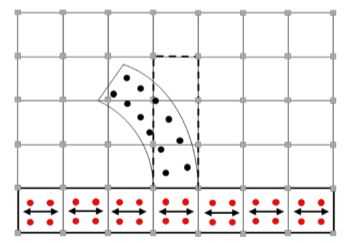
\includegraphics[scale=0.75]{MPM_seismic.jpg}
\caption{Material points prescribed velocity as kinematic boundary condition \cite{Alsardi}}
\label{fig:seismic_method}
\end {figure}
%
%
An experimental study conducted by Hiraoka et al. \cite{Hiraoka} aimed to investigate the influence of seismic shaking on the deformation of a 0.5 m-high sand slope. The sand used in the experiment was partially saturated, with a moisture content of 10 percent. The provided soil parameters for the Mohr Coulomb model include the effective friction angle of 23 degrees, apparent cohesion of 0.78 kPa, Young's modulus of 2.57 MPa, and Poisson's ratio of 0.33, and moist unit weight of 16.5 kN/m3. The soil's dilatancy angle was assumed to be 0 \cite{Hiraoka}. The experimental setup consisted of a shaking table box with a steel horizontal base and smooth glass vertical sidewalls. Laser sensors were used to monitor the displacement of the slope's toe and crest. Figure \ref{fig:vel_profile} displays the velocity-time history employed in the experiment. 
%
%
\begin{figure}[H]
\center
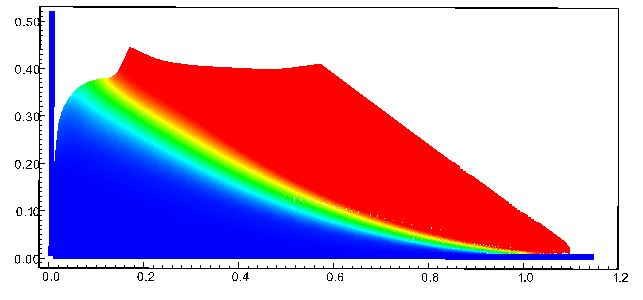
\includegraphics[scale=0.75]{seismic.jpg}
\caption{Numerical model of the seismic-induced slope failure with displacement color}
\label{fig:seismic}
\end {figure}
%
%

To simulate the seismic loading in our numerical model, we adopted a method presented by Alsardi et al. \cite{Alsardi}, which involves specifying the velocity at the corresponding material points representing either the shaking table or the bedrock at the site (see Figure \ref{fig:seismic_method}). In our simulation, we considered the horizontal base to be fully rough and the vertical contact to be fully smooth. The initial stress condition was initiated using gravity and seismic loading induced the slope failure (see Figure \ref{fig:seismic}).\\
Previous studies by Bhandari et al. \cite{Bhandari}, Alsardi et al. \cite{Alsardi}, and Hiraoka et al. \cite{Hiraoka} attempted to model this experiment using MPM and SPH models. In this study, we compared our results with those obtained from other particle-based methods (Figure \ref{fig:Toe}). The main difference is that we did not apply 5 percent numerical damping in our model, unlike the other methods. We found that the final displacement of the slope toe in our MPM model was higher than that observed in the experiment. Nevertheless, the validation of the Mohr-Coulomb model under seismic response demonstrated a reasonable soil behavior in terms of displacement.
%
%
\begin{figure}[H]
\center
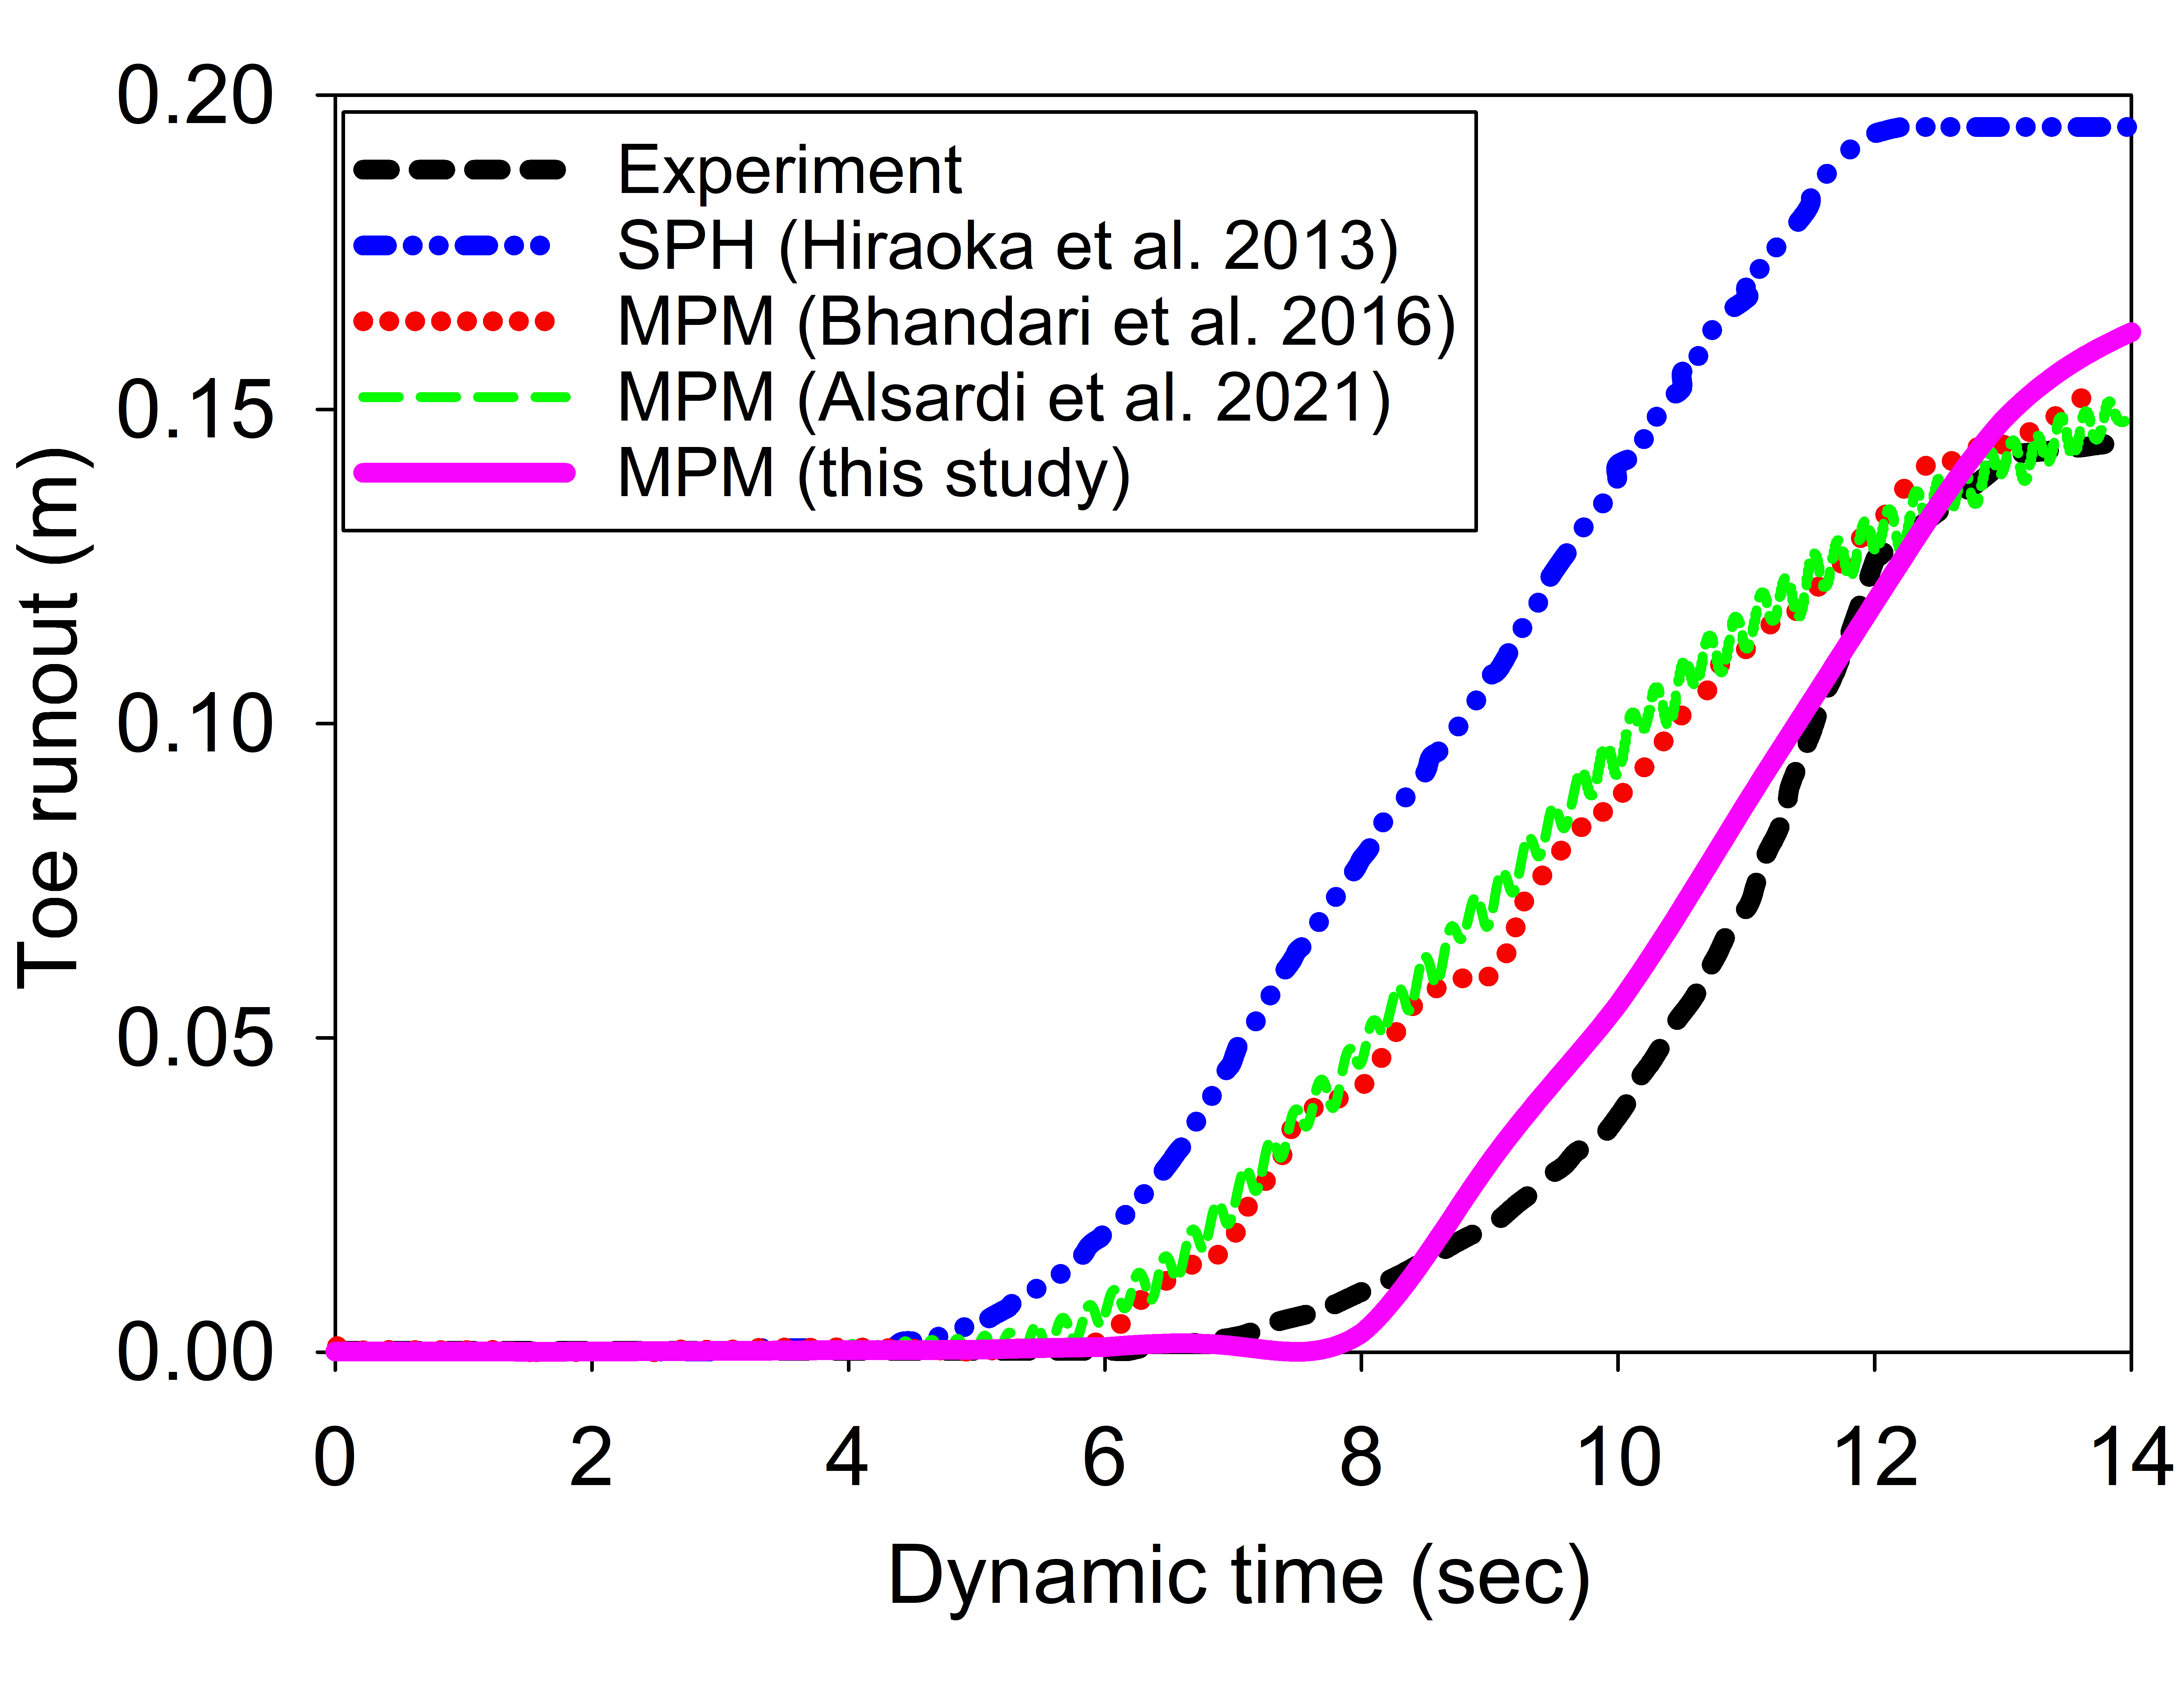
\includegraphics[scale=0.5]{Toe.jpg}
\caption{Displacement of the toe of the slope}
\label{fig:Toe}
\end {figure}
%
%

%_______________________________
\subsection{\textsf{Earthquake-induced submarine landslides}}
%
%
\begin{figure}[H]
\center
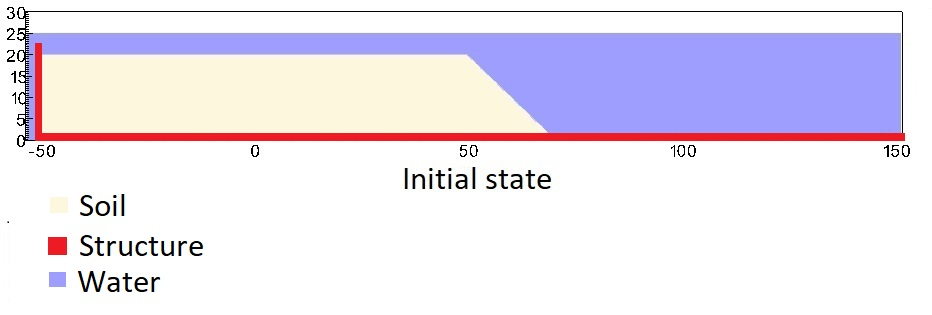
\includegraphics[scale=0.5]{schematic.jpeg}
\caption{Numerical simulation of the earthquake-induced submarine landslide}
\label{fig:scheme}
\end {figure}
%
%
\begin{figure}[H]
\center
%add desired spacing between images, e. g. ~, \quad, \qquad, \hfill etc. 
%(or a blank line to force the subfigure onto a new line)
\begin{subfigure}[c]{0.5\linewidth}
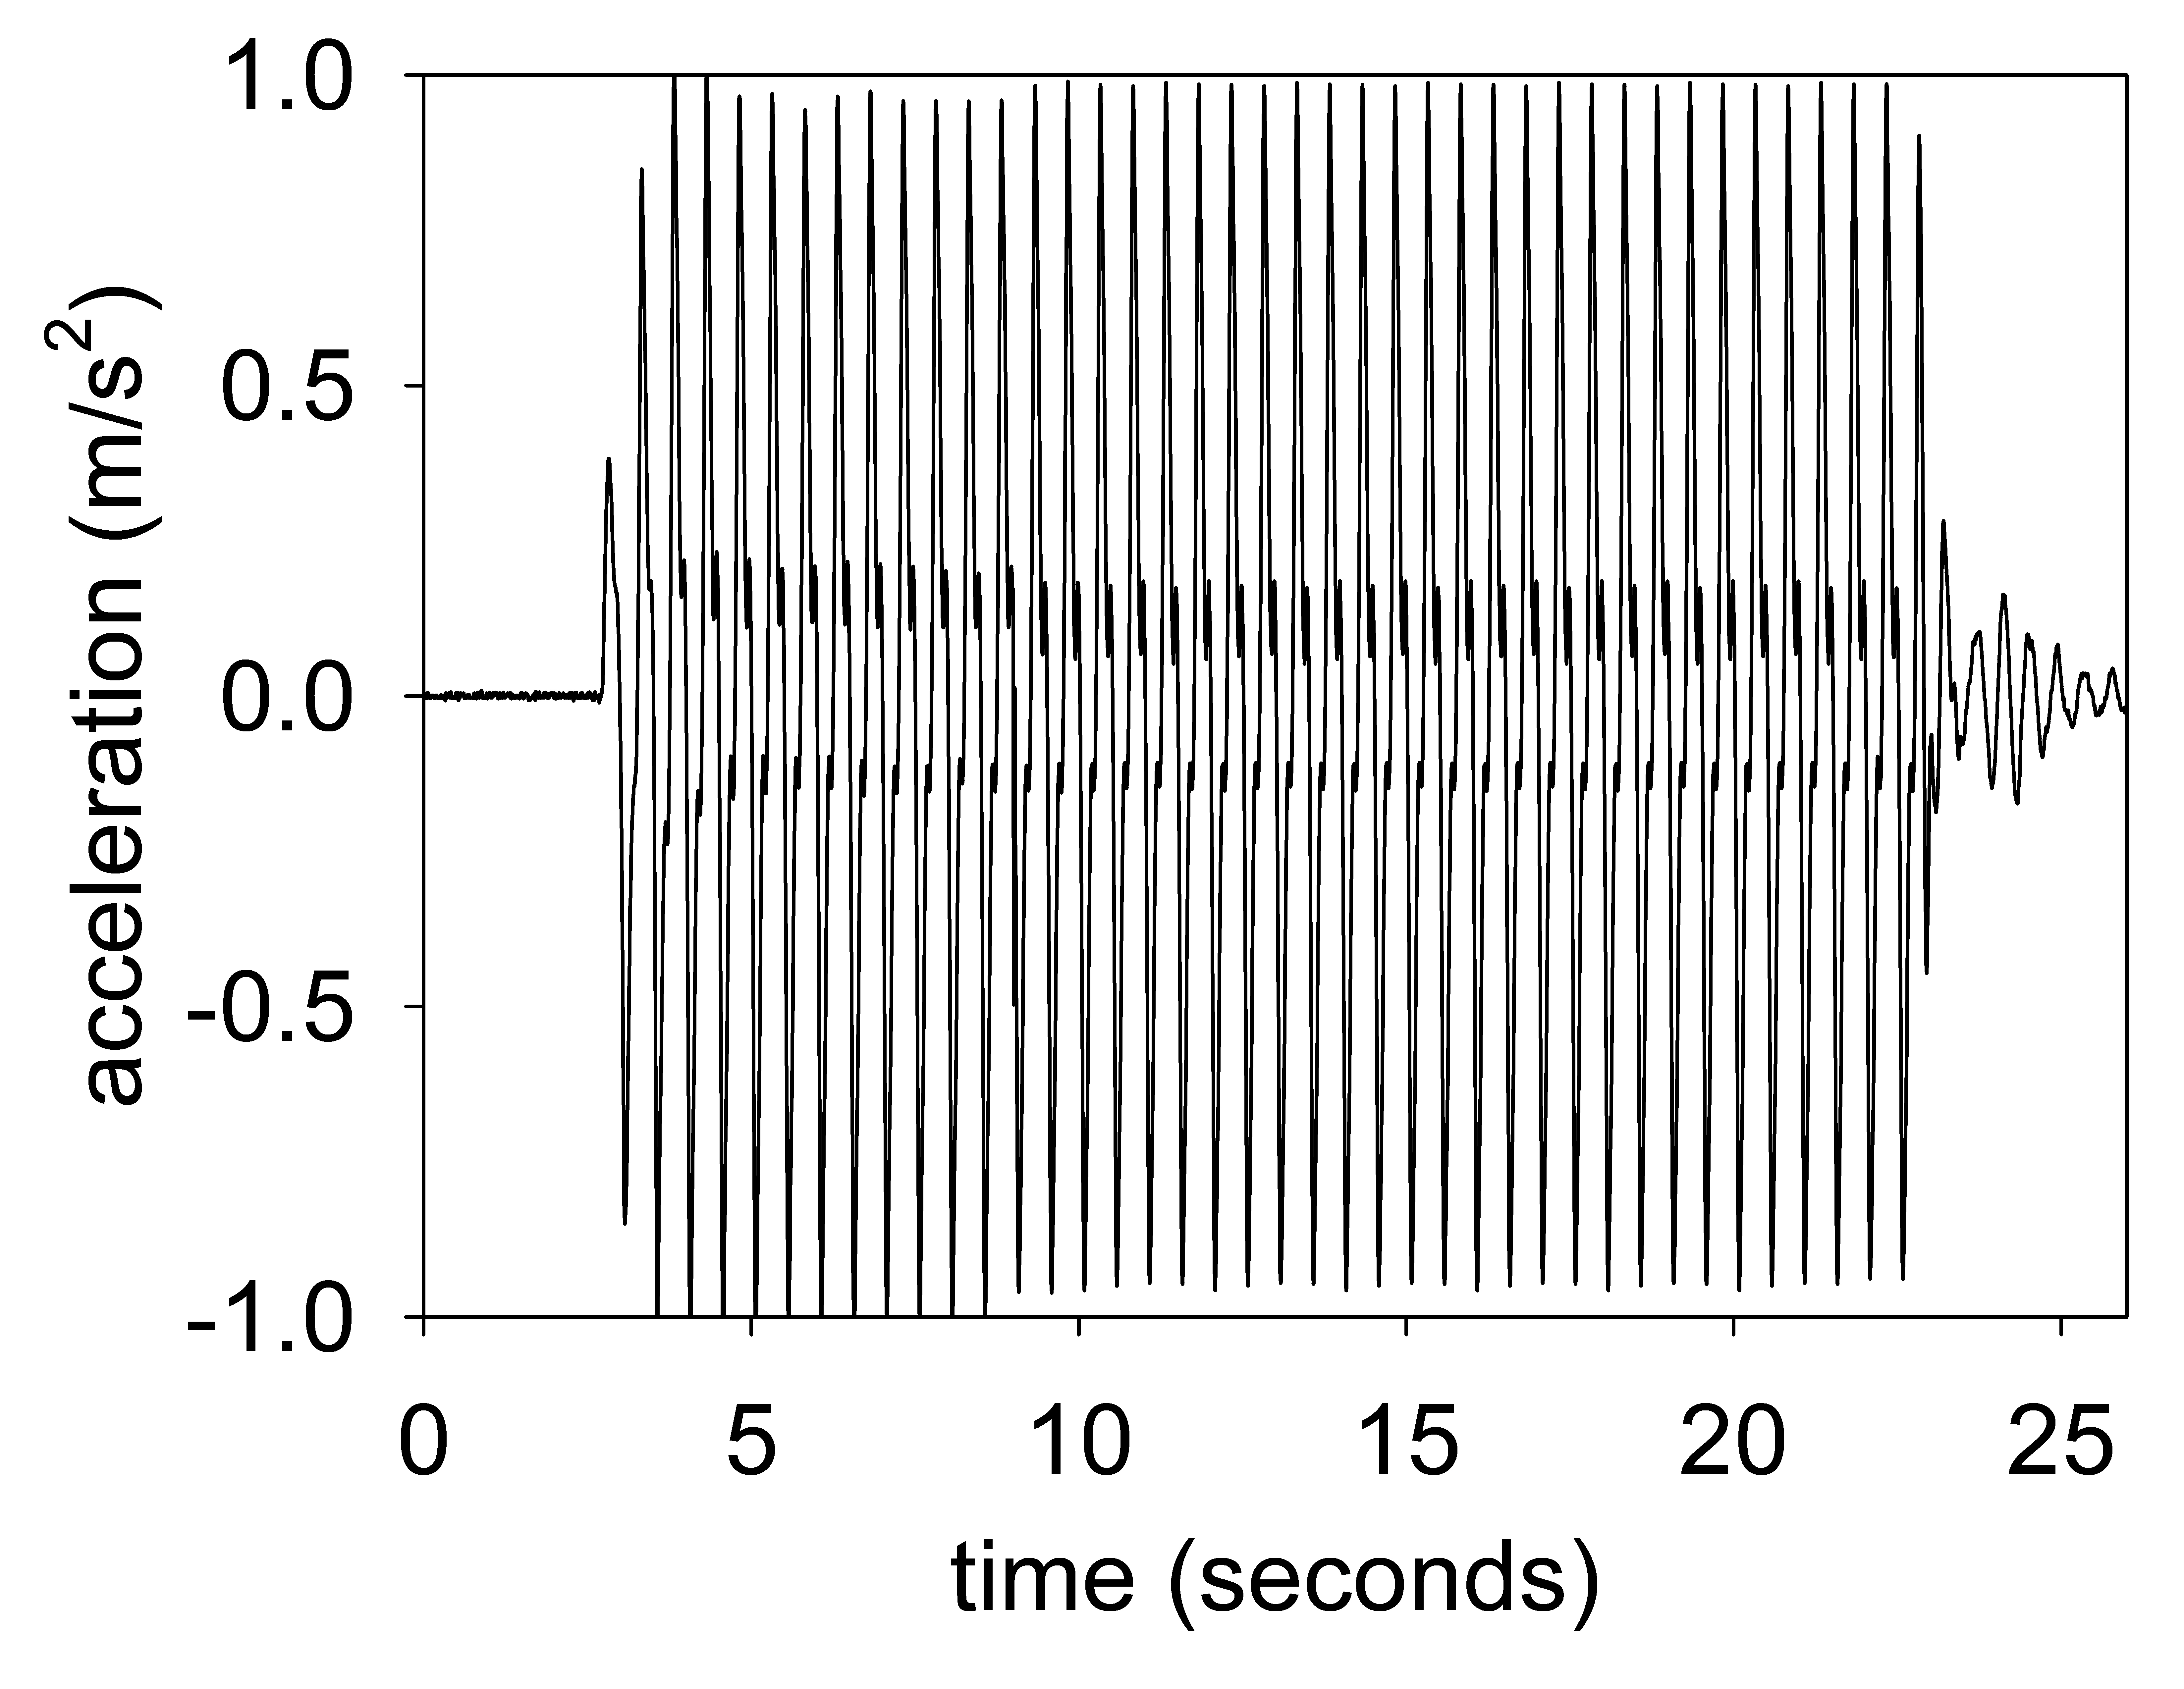
\includegraphics[width=\linewidth]{acer.jpg}
\caption{accerleration}
\label{groundacceleration_accerleration}
\end {subfigure}\hfill    
\begin{subfigure}[d]{0.5\linewidth}
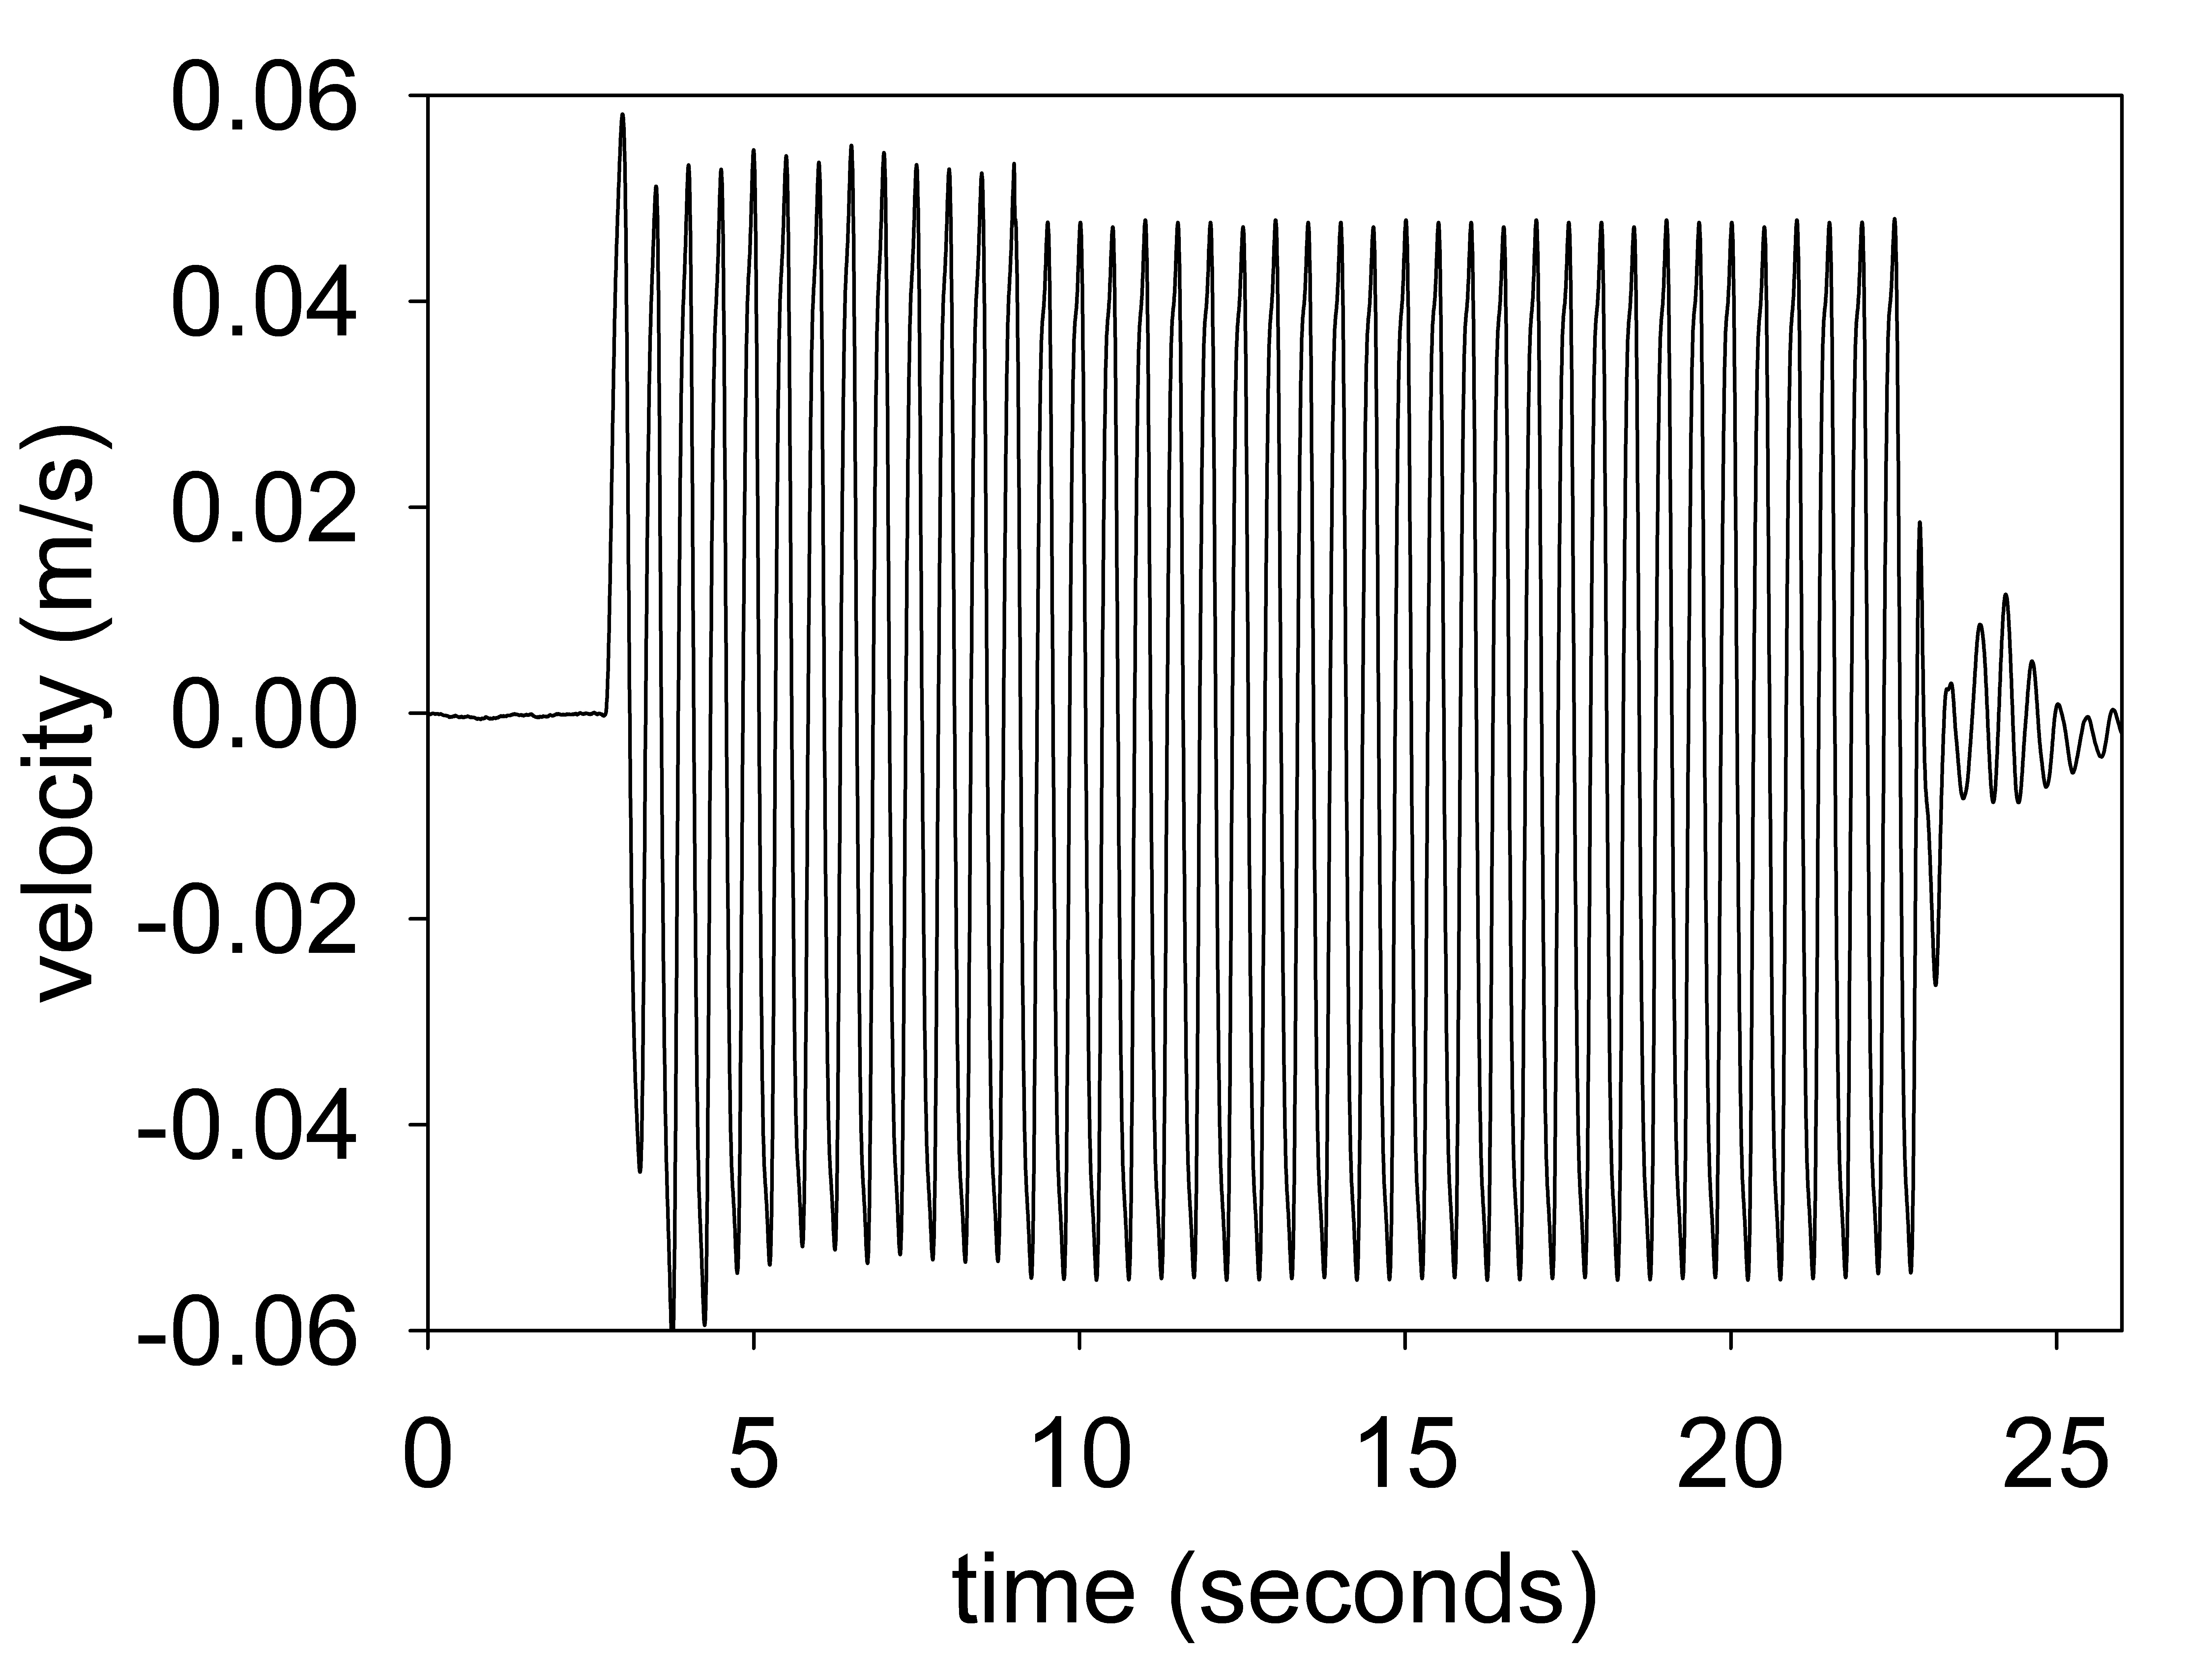
\includegraphics[width=\linewidth]{vel1.jpg}
\caption{velocity}
\label{groundacceleration_velocity}
\end {subfigure}
\caption{Ground acceleration profile, frequency of 2Hz and magnitude of 1g}
\label{groundacceleration}
\end {figure}
In the final example, we perform numerical analysis of the earthquake induced submarine landslides. A plane strain model with the slope under water is shown in Figure \ref{fig:scheme}. A 20m high slope with slope gradient of 45 degrees is placed in a horizontal and vertical structure which was used to be a skaing table to apply earthquake loading. We simplify the earthquake loading by simulating the ground shaking for 20 seconds with the constanct ground acceleration of 1g and a constant frequency of 2Hz (Figure \ref{groundacceleration_accerleration}). The ground motion is applied in terms of velocity (Figure \ref{groundacceleration_velocity}). An earthquake of this magnitude is possible. For instance, in the case of the 2023 Turkey-Syria Earthquake, significant ground shaking with peak ground acceleration exceeding 1g was observed at numerous locations. This serves as an example of the practical occurrence of such high levels of ground acceleration during seismic events. To generate the seismic loading, the same method was used as presented in the previous numerical example.
%
%
\begin{figure}[H]
\center
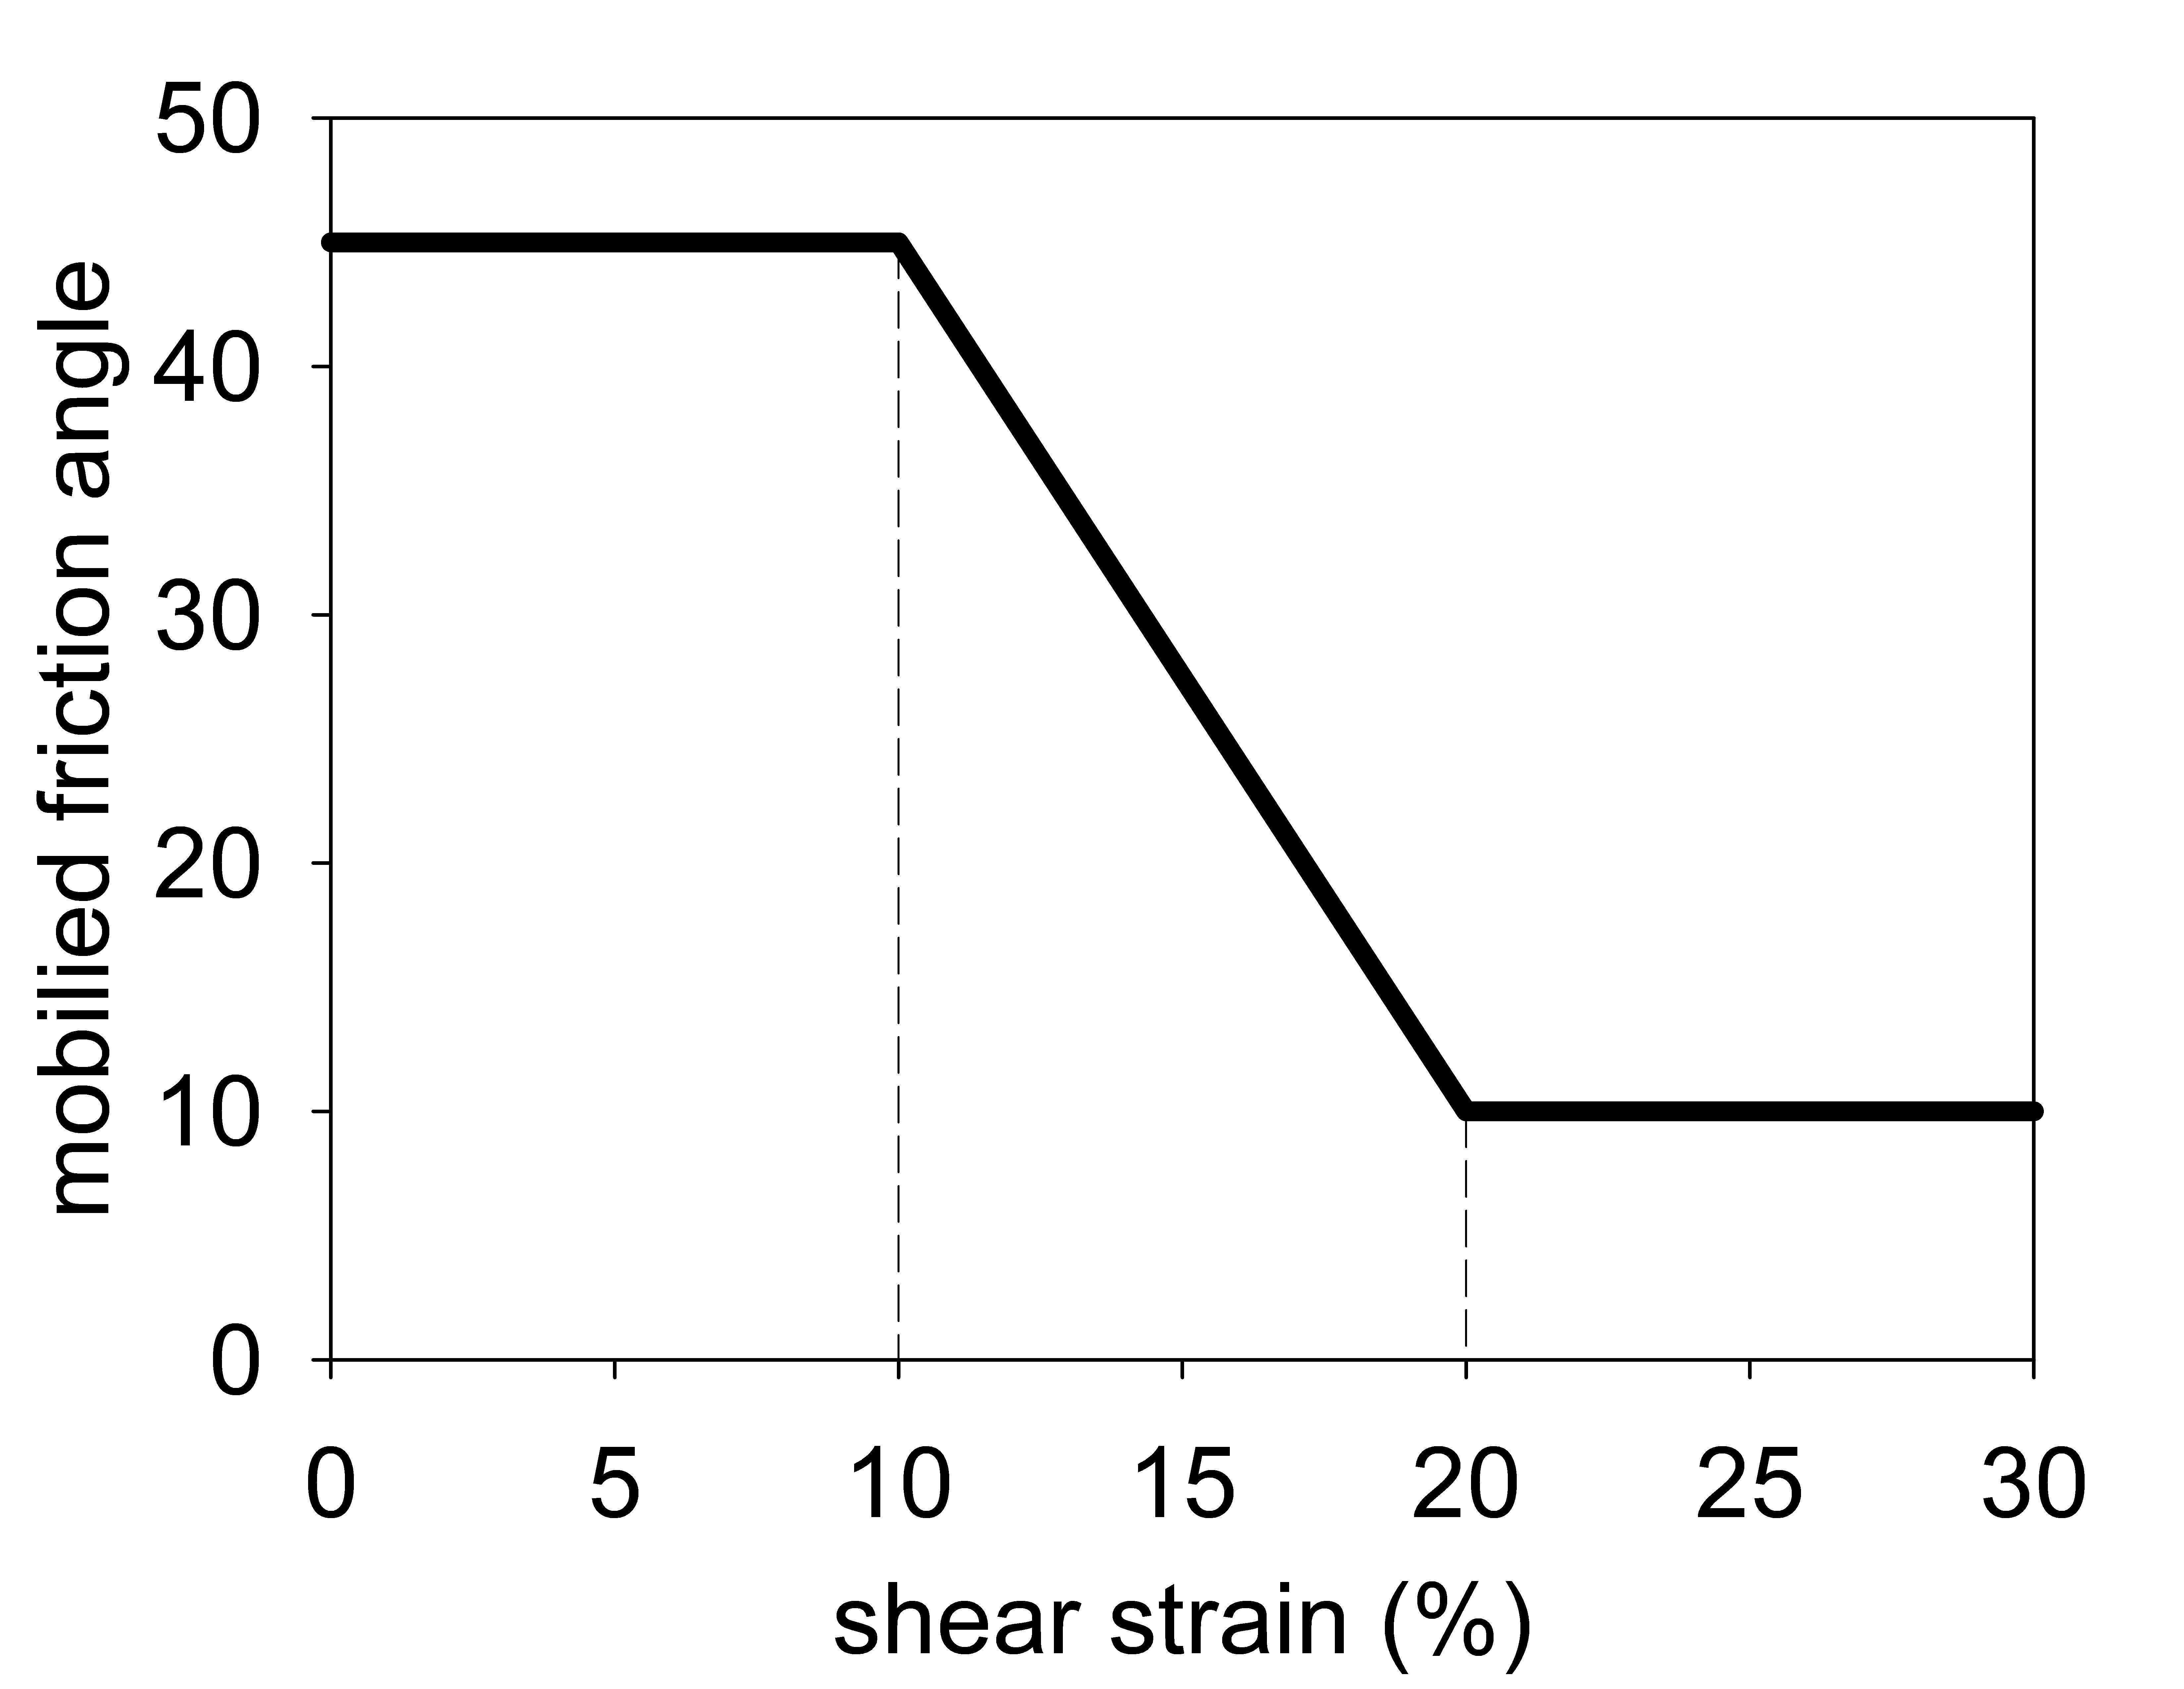
\includegraphics[scale=0.25]{model.jpg}
\caption{Mobilized friction angle in Mohr Coulomb model}
\label{fig:model}
\end {figure}
%
%
A non-associated Mohr-Coulomb model is used for the soil. The soil grain has the density of 2650 kg/$m^3$, Young's modulus of 10 kPa and Poisson's ratio of 0.3 and zero cohesion. The mobilized friction angle $\phi^\prime_m$ is governed following the softening curve (see Figure \ref{fig:model}) with the peak friction angle $\phi^\prime_p$ of 45 degrees and the residual friction angle $\phi^\prime_r$ of 10 degrees. The porosity is 0.3 and the average grain size of the soil is around 0.1 $\mu$m to mimic the undrained behavior. The mobilized dilatancy angle is calculated from the Rowe's stress dilatancy theory  \cite{Wood} as follow:
%
%
\begin{equation}
  \sin{\psi^\prime}_m = \frac{\sin{\phi^\prime}_m - \sin{\phi^\prime}_{r}}{1 - (\sin{\phi^\prime}_{r}\sin{\phi^\prime}_m)}
\end {equation}
%
%
The solid plane is modeled as a rigid body acted as a shaking table. The contact between horizontal plane and the sand is the frictional contact with the friction coefficient of 0.1. No artificial damping is applied in the simulation. The contact between vertical plane and the sand is considered to be smooth with zero friction coefficient. On all boundary faces, the symmetric boundary condition is imposed, while the Neumman boundary condition is imposed at the top boundary for pressure (dp/dx = 0 kPa) and density (d$\rho$/dx = 0 $kg/m^3$). Symmetric boundary condition refers to a condition where the normal component of the velocity at the boundary face is set to zero, and the tangential component is equal to the tangential component of the neighboring cells. The mesh size is 0.25 x 025m with 300852 element cells and 142316 material points. The simulation takes a couple of hours to perform 60 seconds of the simulation using 4096 CPUs.
%
\begin{figure}[H]
\center
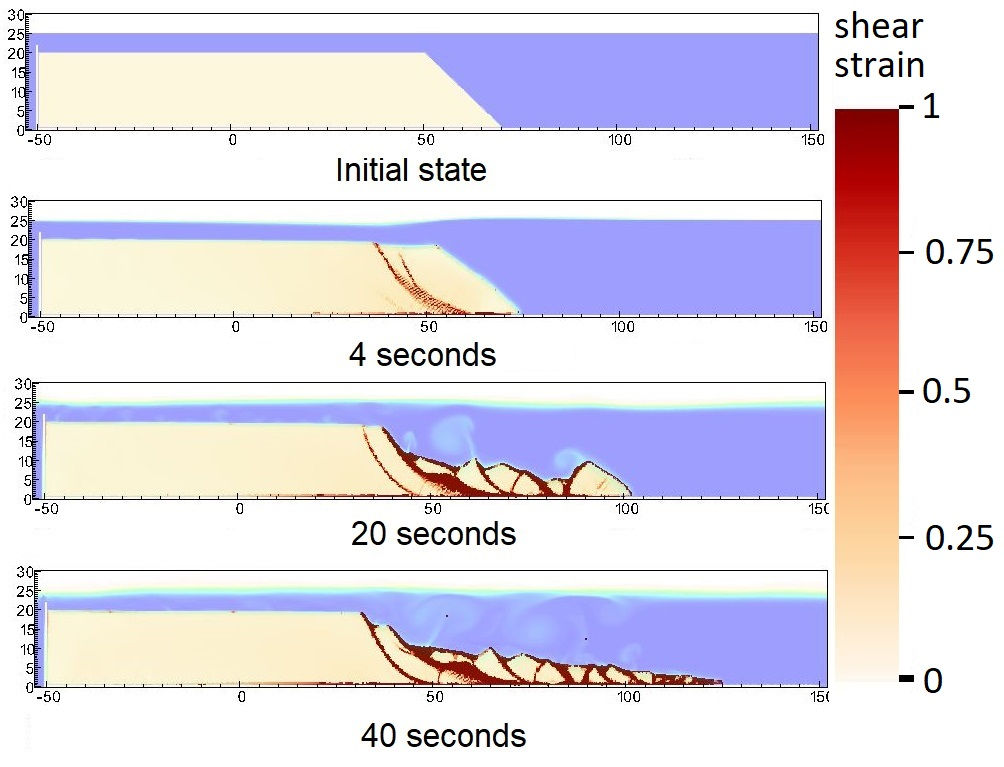
\includegraphics[scale=0.5]{landslide_gamma.jpeg}
\caption{Shear strain during the earthquake-induced submarine landslides}
\label{fig:gamma}
\end {figure}
%
%
We demonstrate the entire process and the mechanism of the earthquake-induced submarine landslides by showing the shear strain (Figure \ref{fig:gamma}), the pore water pressure in atm (Figure \ref{fig:PWP}) and the velocity (Figure \ref{fig:vel}). The failure mechanism can be characterized as the progressive failure mechanism. Here are some numerical observation:
\begin{enumerate}
\item At the initial of the seismic event, the seismic loading triggers the first slide at 3 seconds. At 4 seconds, the debris start to move with the maximum speed of around 2-3 m/s with multiple shear band developed in the slope. The wave generated from the submarine slide is around 2-3m towards the slide direction.
%
\begin{figure}[H]
\center
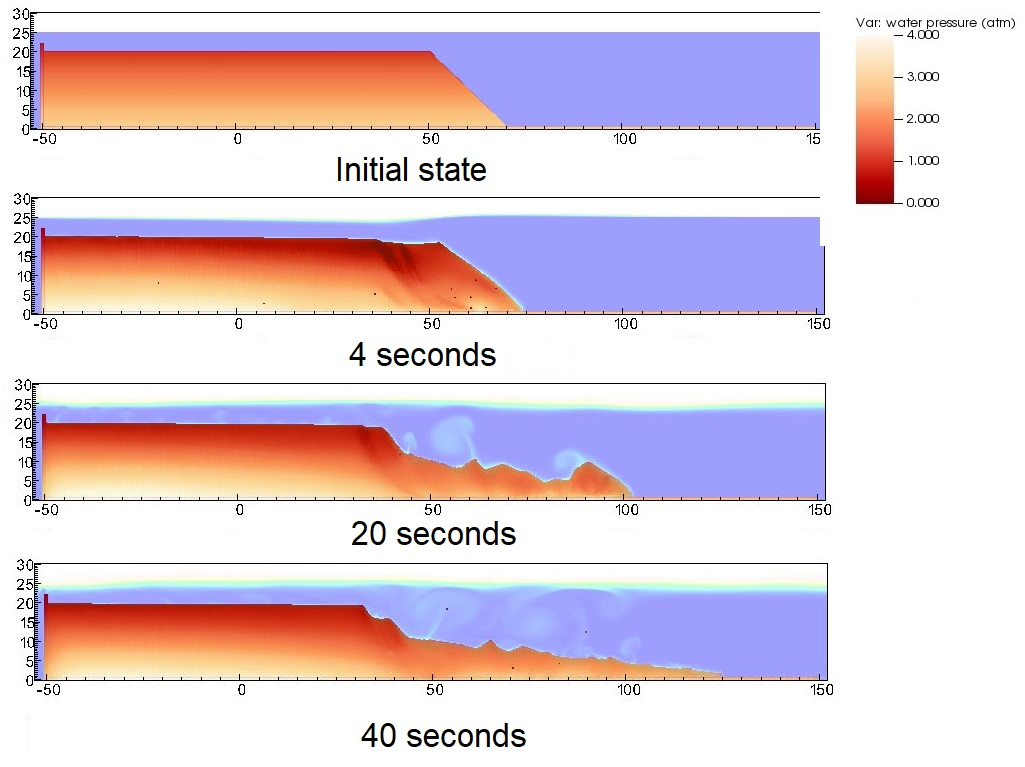
\includegraphics[scale=0.5]{PWP.jpeg}
\caption{pore water pressure during the earthquake-induced submarine landslides}
\label{fig:PWP}
\end {figure}
%
%
\item When the onset of the shear band occurs in the slope (for example at 4 seconds and 20 seconds), the negative excess pore water pressure is developed along this shear band with pore water pressure is under 1atm. This is a typical dilatancy behavior when the soil is sheared rapidly in the undrained behavior. 
\item  When the seismic loading ends at 23 seconds, the last shear band is mobilized and the slope soon reaches to the final deposition. No more progressive failure developed in the slope. The turbulent flow developed as the interaction between debris flow and seawater.
\end {enumerate}
%
Overall, we show the completed process of the earthquake-induced submarine landslides involving (1) earthquake triggering mechanism, (2) the onset of the shear band with the development of negative excess pore water pressure, (3) progressive failure mechanism, (4) submarine landslide induced wave to final deposition.
%
%
\begin{figure}[H]
\center
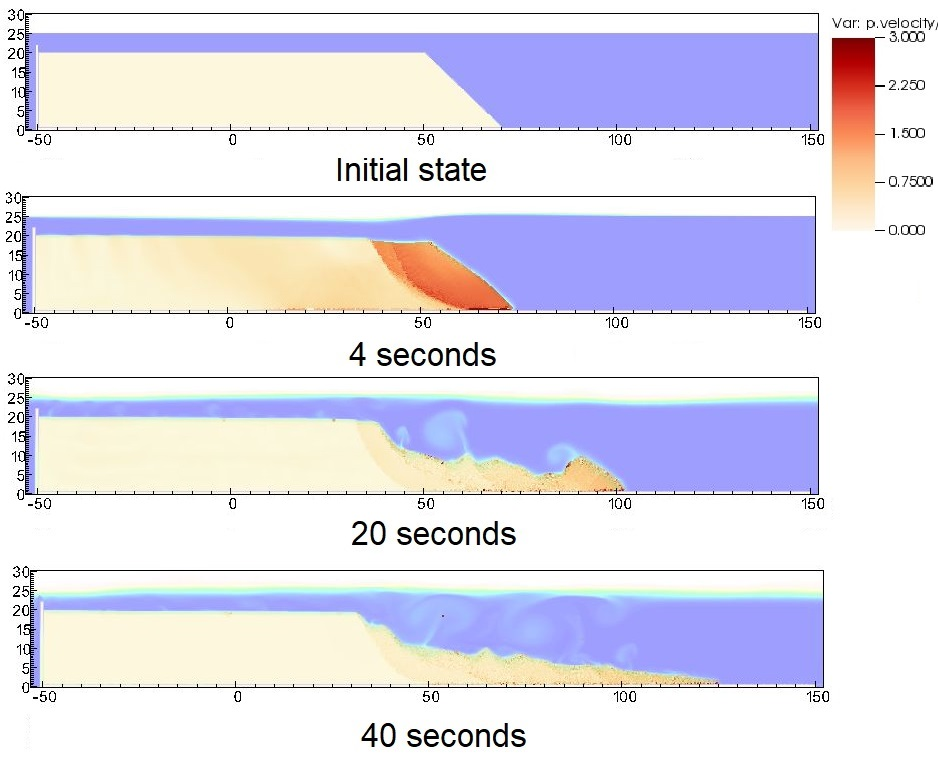
\includegraphics[scale=0.5]{landslide_vel.jpeg}
\caption{Velocity during the earthquake-induced submarine landslides}
\label{fig:vel}
\end {figure}
%
%
%_______________________________
\section{\textsf{Conclusions}}
We have presented a numerical approach MPMICE for the simulation of large deformation soil-fluid-structure interaction, emphasizing the simulation of the earthquake-induced submarine landslides. The model uses (1) the Material Point Method for capturing the large deformation of iso-thermal porous media and solid structures and (2) Implicit Continuous Eulerian (compressible, conservative multi-material CFD formulation) for modeling the complex fluid flow including turbulence. This model is implemented in the high-performance Uintah computational framework and validated against analytical solution and experiment. We then demonstrate the capability of the model to simulate the entire process of the earthquake induced submarine landslides.

%_______________________________
\section{\textsf{Acknowledgements}}
The authors gratefully acknowledge Dr. James Guilkey and Dr. Todd Harman from the University of Utah for sharing the insight on the theoretical framework of MPMICE which this work is based. This project has received funding from the European Union’s Horizon 2020 research and innovation program under the Marie Skłodowska-Curie Actions (MSCA) Individual Fellowship (Project SUBSLIDE “Submarine landslides and their impacts on offshore infrastructures”) grant agreement 101022007. The authors would also like to acknowledge the support from the Research Council of Norway through its Centers of Excellence funding scheme, project number 262644 Porelab. The computations were performed on High Performance Computing resources provided by UNINETT Sigma2 - the National Infrastructure for High Performance Computing and Data Storage in Norway.

%_______________________________
%\appendix

\section{\textsf{Appendix: Equation derivation}}
%
%
Before deriving the governing equation, we define the Lagrangian derivative for a state variable $f$ as:
%
%
\begin{equation}
\frac{D_f f}{Dt} =  \frac{\partial f}{\partial t} + \pmb{U_f} \cdot \nabla f \qquad
\frac{D_s f}{Dt} =  \frac{\partial f}{\partial t} + \pmb{U_s} \cdot \nabla f
\end {equation}
%
%
we use some definition following \cite{Kashiwa} as below:
%
%
\begin{gather}
-\frac{1}{V} \left[ \frac{\partial V_f}{\partial p} \right] \equiv \kappa_f \qquad \mbox{ isothermal compressibility of fluid} \\
\frac{1}{V} \left[ \frac{\partial V_f}{\partial T} \right] \equiv \alpha_f \qquad \mbox{ contant pressure thermal expansivity of fluid}
\end {gather}
%
%
Then, the rate of volume with incompressible solid grains are calculated as belows:
%
%
\begin{equation}
\label{fluidvolumerate}
\begin{gathered}
   \frac{1}{V} \frac{D_f V_f}{Dt} = \frac{1}{V} \left( \left[ \frac{\partial V_f}{\partial p} \right] \frac{D_f P_{eq}}{D t} + \left[ \frac{\partial V_f}{\partial T_f} \right] \frac{D_f T}{D t} \right) = \frac{1}{V} \left( -\kappa_f \frac{D_f P_{eq}}{D t} + \alpha_f \frac{D_f T_f}{D t} \right) \\
\end {gathered}
\end {equation}
%
%
\subsection{\textsf{Evolution of porosity}}
%
%
Solving the solid mass balance equation (\ref{massbalance}) with the definition of solid mass in equation (\ref{mass}), it leads to the rate of porosity as belows:
%
%
\begin{equation}
   \frac{D_sm_s}{Dt} = \frac{D_s(\phi_s \rho_s V)}{Dt} = \rho_s V \frac{D_s \phi_s}{Dt} + \phi_s V \frac{D_s \rho_s}{Dt} + \phi_s \rho_s  \frac{D_s V}{Dt} = 0  
\end {equation}
%
%
The soil grains are assumed to be incompressible, therefore, term 2 in the right hand side is zero. leading to:
%
%
\begin{equation}
  V \frac{D_s \phi_s}{Dt} + \phi_s \frac{D_s V}{Dt} = 0  
\end {equation}
%
%
Dividing all terms with $V$ with the equation $\frac{1}{V} \frac{D_s V}{Dt} = \nabla \cdot \pmb{U}_s $, it leads to:
%
%
\begin{equation}
  \frac{D_s n}{Dt} = \frac{\partial n}{\partial t} + \pmb{U}_s \cdot \nabla n = 
  \phi_s \nabla \cdot \pmb{U}_s  
\end {equation}
%
%
\subsection{\textsf{Momentum conservation}}
\label{Momentum}
%
%
The linear momentum balance equations for the fluid phases based on mixture theory are:\\
%
%
\begin{equation}
    \frac{1}{V}\frac{D_f(m_f \pmb{U}_f)}{Dt} = 
    \nabla \cdot (-\phi_f p_f\pmb{I}) + \nabla \cdot \pmb{\tau}_f + \overline{\rho}_f \pmb{b} +  \sum \pmb{f}_{d} + \pmb{f}_b
\end {equation}
%
%
On the right hand sand, the first term is the divergence of partial fluid phase stress, the third term is the body force, the fourth term is the drag force (momentum exchange) and the fifth term is the buoyant force described in \cite{DRUMHELLER} for the immiscible mixtures. The buoyant force is in the form as belows:
%
%
\begin{equation}
    \pmb{f}_b = \pmb{\sigma}_f\nabla (n)
\end {equation}
%
%
As a result, the linear momentum balance equations for the fluid phases become as:
%
%
\begin{equation}
    \label{fluidmom}
     \frac{1}{V}\frac{D_f(m_f \pmb{U}_f)}{Dt} =  \frac{1}{V} \left[ \frac{\partial (m_f \pmb{U}_f)}{\partial t} + \nabla \cdot  (m_f \pmb{U}_f \pmb{U}_f) \right] = -\phi_f \nabla p_f + \nabla \cdot \pmb{\tau}_f +  \overline{\rho}_f \pmb{b} +  \sum  \pmb{f}_{d}
\end {equation}
%
%
The Reynolds stress component can be included in the term $\pmb{\tau}_f$ to consider the turbulent effects if needed. To derive the linear momentum balance equation for the solid phase, we begin with the linear momentum balance equation for the mixture as:
%
%
\begin{equation}
    \label{totalmom}
     \frac{1}{V}\frac{D_f(m_f \pmb{U}_f)}{Dt}
    +  \frac{1}{V}\frac{D_s(m_s \pmb{U}_s)}{Dt} = 
    \nabla \cdot (\pmb{\sigma}) + \overline{\rho}_f \pmb{b} 
    + \overline{\rho}_s \pmb{b}
\end {equation}
%
%
Combining Terzaghi's equation (\ref{Terzaghi}) and subtracting both sides with equation (\ref{fluidmom}), we obtain the linear momentum balance equations for the solid phase as:
%
%
\begin{equation}
    \label{solidmom}
     \frac{1}{V}\frac{D_s(m_s \pmb{U}_s)}{Dt} = 
    \nabla \cdot (\pmb{\sigma}^\prime) - \phi_s \nabla p_f 
    + \overline{\rho}_s \pmb{b}   -  \sum \pmb{f}_{d} +  \sum \pmb{f}_{fric}
\end {equation}
%
%
Here the $\pmb{f}_{fric}$ stems from the soil-structure interaction following the contact law between the soil/structure interfaces.
\subsection{\textsf{Energy conservation}}
We adopt the general form of the total energy balance equation for the porous media from \cite{Hassanizadeh}, the total energy balance equations for the fluid phases are:
%
%
\begin{equation}
\label{e1}
     \frac{1}{V}\frac{D_f(m_f (e_f+0.5\pmb{U}_f^2))}{Dt} = \nabla \cdot (-np_f\pmb{I}) \cdot \pmb{U}_f + \nabla \cdot \pmb{q}_f + (\overline{\rho}_f \pmb{b}) \cdot \pmb{U}_f +  \sum \pmb{f}_{d} \cdot \pmb{U}_f +  \sum q_{sf}
\end {equation}
%
%
Applying the product rule $D(m\pmb{U}^2)=D(m \pmb{U} \cdot \pmb{U}) = 2 \pmb{U} \cdot D(m \pmb{U})$, the left hand side of equation (\ref{e1}) becomes:\\
%
%
\begin{equation}
\label{e2}
     \frac{1}{V}\frac{D_f(m_f (e_f+0.5\pmb{U}_f^2))}{Dt}  = \frac{1}{V}\frac{D_f(m_f e_f)}{Dt} + \frac{1}{V}\frac{D_f(m_f \pmb{U}_f)}{Dt} \cdot \pmb{U}_f 
\end {equation}
%
%
Combining equations (\ref{fluidmom}), (\ref{e1}), (\ref{e2}), we obtain the final form of the internal energy balance equation for the fluid phases as:
%
%
\begin{equation}
     \frac{1}{V}\frac{D_f(m_f e_f)}{Dt} = \frac{1}{V} \left[ \frac{\partial (m_f e_f)}{\partial t} + \nabla \cdot  (m_f e_f \pmb{U}_f) \right] 
   = \overline{\rho}_f p_f  \frac{D_f\upsilon_f}{Dt} + \nabla \cdot \pmb{q}_f +  \sum q_{sf}
\end {equation}
%
%
On the right hand side, the terms include the average pressure-volume work, the average viscous dissipation, the thermal transport and the energy exchange between solid and fluid respectively. The heat flux is $\pmb{q}_f = \overline{\rho}_f \beta_f \nabla T_f$ with $\beta_f$ being the thermal conductivity coefficient. To derive the internal energy balance equation for the solid phase, we introduce the rate of the internal energy  for the thermoelastic materials as a function of elastic strain tensor $\pmb{\epsilon}_s^e$ and temperature $T_s$ as belows:
%
%
\begin{equation}
   \frac{m_s}{V} \frac{D_s( e_s)}{Dt} = \pmb{\sigma}^\prime :\frac{D_s( \pmb{\epsilon}_s^e)}{Dt} + \frac{D_s( e_s)}{D_s (T_s)} \frac{D_s( T_s)}{Dt} = \pmb{\sigma}^\prime :\frac{D_s( \pmb{\epsilon}_s^e)}{Dt} + c_v \frac{D_s( T_s)}{Dt}
\label{internalEnergy}
\end {equation}
%
%
$c_v$ is the specific heat at the constant volume of the solid materials. The total energy balance equation for the mixture based on \cite{Hassanizadeh} can be written as:\\
%
%
\begin{equation}
\label{e3}
\begin{gathered}
     \frac{1}{V}\frac{D_f(m_f (e_f+0.5\pmb{U}_f^2))}{Dt} + \frac{1}{V}\frac{D_s(m_s (e_s+0.5\pmb{U}_s^2))}{Dt} = \nabla \cdot (-\phi_f p_f\pmb{I}) \cdot \pmb{U}_f \\
     + \nabla \cdot (\pmb{\sigma}^\prime-\phi_s p_f\pmb{I}) \cdot \pmb{U}_s + (-\phi_f p_f\pmb{I}) : \nabla \pmb{U}_f + \pmb{\sigma}^\prime : \nabla \pmb{U}_s \\
     + (\overline{\rho}_f \pmb{b}) \cdot \pmb{U}_f + (\overline{\rho}_s \pmb{b}) \cdot \pmb{U}_s
     + \nabla \cdot \pmb{q}_f + \nabla \cdot \pmb{q}_s +  \sum \pmb{f}_{d} \cdot (\pmb{U}_f - \pmb{U}_s)  
\end {gathered}
\end {equation}
%
%
Subtracting equation (\ref{e3}), (\ref{internalEnergy}) to equations (\ref{e1}) and (\ref{solidmom}), we obtained the internal energy balance equation for solid phase as:
%
%
\begin{equation}
      \pmb{\sigma}^\prime :\frac{D_s( \pmb{\epsilon}_s^e)}{Dt}  + \frac{m_s}{V} c_v \frac{D_s( T_s)}{Dt} = \Delta W_{s} +  \Delta W_{friction} + \nabla \cdot \pmb{q}_s -  \sum q_{sf} 
\end {equation}
%
%
On the right hand side, the terms include the work rate from frictional sliding between solid materials  $\Delta W_{friction}$, thermal transport and energy exchange between solid and fluid respectively. The heat flux is $\pmb{q}_s = \overline{\rho}_s \beta_s \nabla T_s$ with $\beta_s$ being the thermal conductivity of the solid materials, the mechanical work rate $\Delta W_{s} = \pmb{\sigma}^\prime :\frac{D_s( \pmb{\epsilon}_s)}{Dt}  = \pmb{\sigma}^\prime : (\frac{D_s( \pmb{\epsilon}_s^e)}{Dt}  + \frac{D_s( \pmb{\epsilon}_s^p)}{Dt}) $ computed from the constitutive model with $\pmb{\epsilon}_s^p$ is the plastic strain tensor, . By subtracting the term $\pmb{\sigma}^\prime : \frac{D_s( \pmb{\epsilon}_s^e)}{Dt}$, we get the final form of the energy balance equation as:
%
%
\begin{equation}
      \frac{m_s}{V} c_v \frac{D_s( T_s)}{Dt} = \pmb{\sigma}^\prime : \frac{D_s( \pmb{\epsilon}_s^p)}{Dt} +  \Delta W_{friction} + \nabla \cdot \pmb{q}_s -  \sum q_{sf} 
\end {equation}
%
%
\subsection{\textsf{Advanced Fluid Pressure}}
The discretization of the pressure equation begins with the Lagrangian cell face velocity and the equation for the pressure as:
%
\begin{equation}
 \label{append:pressure1}
  \overline{\rho}_{f,FC} \frac{\pmb{U}_{f,FC}^{n+1} - \pmb{U}_{f,FC}^{n}}{dt} 
  = n \nabla^{FC} P_{f,c}^{n+1} + \overline{\rho}_{f,FC} \pmb{b}
\end {equation}
%
%
\begin{equation}
\label{append:pressure2}
  \kappa \frac{dP}{dt} = \nabla^c \cdot \pmb{U}_{f,FC}^{n+1}
\end {equation}
%
The divergence of the equation (\ref{append:pressure1}) with $ \nabla \cdot \pmb{b} = 0$ is:
%
\begin{equation}
\label{append:pressure3}
  \nabla^c \cdot \pmb{U}_{f,FC}^{n+1} - \nabla^c \cdot \pmb{U}_{f,FC}^{n}
  = \nabla^c \frac{\delt}{\rho_{f,FC}^n} \cdot \nabla^{FC} (P_{f,c}^{n} + \Delta P_{f,c}^{n})
\end {equation}
%
To solve this equation, we define the cell face intermediate velocity $ \pmb{U}_{f,FC}^{*}$ as:
%
\begin{equation}
 \label{append:pressure4}
  \overline{\rho}_{f,FC} \frac{\pmb{U}_{f,FC}^{*} - \pmb{U}_{f,FC}^{n}}{\delt} 
  = n \nabla^{FC} P_{f,c}^{n} + \overline{\rho}_{f,FC} \pmb{b}
\end {equation}
%
%
The divergence of the equation (\ref{append:pressure4}) is:
%
\begin{equation}
\label{append:pressure5}
  \nabla^c \cdot \pmb{U}_{f,FC}^{*} - \nabla^c \cdot \pmb{U}_{f,FC}^{n}
  = \nabla^c \frac{\delt}{\rho_{f,FC}^n} \cdot \nabla^{FC} P_{f,c}^{n}
\end {equation}
%
Combining equations (\ref{append:pressure2}, \ref{append:pressure3}, \ref{append:pressure5}), it leads to:
\begin{equation}
\label{append:pressure6}
  \left(  
   \kappa - \nabla^c \frac{\delt}{\rho_{f,FC}^n} \cdot \nabla^{FC}
  \right) \Delta P_{fc}^{n} = - \nabla^c \cdot \pmb{U}_{f,FC}^{*}
\end {equation}
When the fluid is incompressible, $\kappa$ approaches to zero and the equation (\ref{append:pressure6}) becomes the Poisson's equation for the incompressible fluid flow.
%
%
\subsection{\textsf{Momentum and Energy exchange with an implicit solver}}
%
%
Considering the fluid momentum balance equation as: 
%
\begin{equation}
  (m\pmb{U})_{f,FC}^{n+1} =  (m\pmb{U})_{f,FC}^{n} - \delt (V n \nabla^{FC} P_{f,c}^{n} + m_f \pmb{b}) + V K \delt (\pmb{U}_{s,FC}^{n+1} - \pmb{U}_{f,FC}^{n+1})
\end {equation}
%
%
And assuming $m_{f,FC}^{n+1} = m_{f,FC}^n$, we get:
%
\begin{equation}
  \pmb{U}_{f,FC}^{n+1} =  \pmb{U}_{f,FC}^{n} - \delt (\frac{\nabla^{FC} P_{fc}^{n}} {\rho_{f,FC}^n} + \pmb{b}) + \frac{\delt K}{\overline{\rho}_{f,FC}^n} (\pmb{U}_{s,FC}^{n+1} - \pmb{U}_{f,FC}^{n+1})
\end {equation}
%
%
As defined in the section 'Advanced Fluid Pressure', the cell face intermediate fluid velocity $\pmb{U}_{f,FC}^{*} = \delt (\nabla^{FC} P_{fc}^{n} / \rho_{f,FC}^n + \pmb{b})$ is computed as:
%
\begin{equation}
\label{append:exchange1}
  \pmb{U}_{f,FC}^{n+1} =  \pmb{U}_{f,FC}^{*} +  \frac{\delt K}{\overline{\rho}_{f,FC}^n} (\pmb{U}_{s,FC}^{n+1} - \pmb{U}_{f,FC}^{n+1})
\end {equation}
%
%
Considering the solid momentum balance equation as:
%
\begin{equation}
  (m\pmb{U})_{s,FC}^{n+1} =  (m\pmb{U})_{s,FC}^{n} - \delt (V \nabla^{FC} \cdot \pmb{\sigma}^{'n} - V (1-n) \nabla^{FC} P_{f,c}^{n} + m_s \pmb{b}) - V K \delt (\pmb{U}_{s,FC}^{n+1} - \pmb{U}_{f,FC}^{n+1})
\end {equation}
%
%
We define the cell face intermediate solid velocity as $\pmb{U}_{s,FC}^{*} = \delt (\nabla^{FC} \cdot \pmb{\sigma}_c^{'n} / \overline{\rho}_{s,FC}  - \nabla^{FC} P_{f,c}^{n} / \rho_s + \pmb{b})$ leading to:
%
\begin{equation}
\label{append:exchange2}
  \pmb{U}_{s,FC}^{n+1} =  \pmb{U}_{s,FC}^{*} -  \frac{\delt K}{\overline{\rho}_{s,FC}^n} (\pmb{U}_{s,FC}^{n+1} - \pmb{U}_{f,FC}^{n+1})
\end {equation}
%
%
Combining equation (\ref{append:exchange1}) and (\ref{append:exchange2}) we get:
%
\begin{equation}
\begin{gathered}
\label{append:exchange3}
  \pmb{U}_{f,FC}^{*} + \Delta \pmb{U}_{f,FC} =  \pmb{U}_{f,FC}^{*} +  \frac{\delt K}{\overline{\rho}_{f,FC}^n} (\pmb{U}_{s,FC}^{*} + \Delta \pmb{U}_{s,FC} - \pmb{U}_{f,FC}^{*} - \Delta \pmb{U}_{f,FC}) \\
  \pmb{U}_{s,FC}^{*} + \Delta \pmb{U}_{s,FC} =  \pmb{U}_{s,FC}^{*} -  \frac{\delt K}{\overline{\rho}_{s,FC}^n} (\pmb{U}_{s,FC}^{*} + \Delta \pmb{U}_{s,FC} - \pmb{U}_{f,FC}^{*} - \Delta \pmb{U}_{f,FC})
\end {gathered}
\end {equation}
%
%
Rearranging the equation (\ref{append:exchange3}), it leads to the linear system of equations as belows:
%
\[ \begin{vmatrix} (1 + \beta_{12,FC})  &  -\beta_{12,FC} \\
                  -\beta_{21,FC}       &  (1 + \beta_{21,FC})
    \end {vmatrix}
    \begin{vmatrix} \Delta \pmb{U}_{f,FC} \\
                    \Delta \pmb{U}_{s,FC}
    \end {vmatrix}
    =
    \begin{vmatrix}  \beta_{12,FC}(\pmb{U}_{s,FC}^{*} - \pmb{U}_{f,FC}^{*}) \\
                    \beta_{21,FC}(\pmb{U}_{f,FC}^{*} - \pmb{U}_{s,FC}^{*})
    \end {vmatrix}                
\]
%
%
Solving this linear equations with $\beta_{12,FC} = (\delt K)/\overline{\rho}_{f,FC}^n$ and $\beta_{21,FC} = (\delt K)/\overline{\rho}_{s,FC}^n$ with K is the momentum exchange coefficient. Similar derivation can be performed to computed the cell-center velocity increment leading to:
%
\[ \begin{vmatrix} (1 + \beta_{12c})  &  -\beta_{12c} \\
                  -\beta_{21c}       &  (1 + \beta_{21c})
    \end {vmatrix}
    \begin{vmatrix} \Delta \pmb{U}_{f,c} \\
                    \Delta \pmb{U}_{sc}
    \end {vmatrix}
    =
    \begin{vmatrix}  \beta_{12c}(\pmb{U}_{sc}^{*} - \pmb{U}_{f,c}^{*}) \\
                    \beta_{21c}(\pmb{U}_{f,c}^{*} - \pmb{U}_{sc}^{*})
    \end {vmatrix}                
\]
%
%
with $\beta_{12c} = (\delt K)/\overline{\rho}_{f,c}^n$ and $\beta_{21c} = (\delt K)/\overline{\rho}_{sc}^n$ and the cell-centered intermediate velocity can be calculated by:
%
\begin{equation}
\begin{gathered}
\pmb{U}_{f,c}^{*} = \pmb{U}_{f,c}^{n} + \delt (-\frac{\nabla P_{f,c}^{n+1}}{\rho_{f,c}^n}  + \frac {\nabla \cdot \pmb{\tau}_{f,c}^{n}}{\overline{\rho}^n_{f,c}} + \pmb{b}) \\
\pmb{U}_{sc}^{*} = \pmb{U}_{sc}^{n} + \delt (\frac{\nabla \cdot \pmb{\sigma}_c^{'n}}{\overline{\rho}^n_{sc}}    - \frac{\nabla P_{f,c}^{n+1}}{\rho_s}  + \pmb{b})
\end {gathered}
\end {equation}
%
For generalize multi materials i,j = 1:N, the linear equations is in the form as:
%
%
\[ \begin{vmatrix} (1 + \beta_{ij})  &  -\beta_{ij} \\
                  -\beta_{ji}       &  (1 + \beta_{ji})
    \end {vmatrix}
    \begin{vmatrix} \Delta \pmb{U}_{i} \\
                    \Delta \pmb{U}_{j}
    \end {vmatrix}
    =
    \begin{vmatrix}  \beta_{ij}(\pmb{U}_{i}^{*} - \pmb{U}_{j}^{*}) \\
                    \beta_{ji}(\pmb{U}_{j}^{*} - \pmb{U}_i^{*})
    \end {vmatrix}                
\]
Similar approach applied for the ernergy exchange term leading to:
%
%
\[ \begin{vmatrix} (1 + \eta_{ij})  &  -\eta_{ij} \\
                  -\eta_{ji}       &  (1 + \eta_{ji})
    \end {vmatrix}
    \begin{vmatrix} \Delta T_{i} \\
                    \Delta T_{j}
    \end {vmatrix}
    =
    \begin{vmatrix}  \eta_{ij}(T_{i}^{n} - T_{j}^{n}) \\
                    \eta_{ji}(T_{j}^{n} - T_i^{n})
    \end {vmatrix}                
\]
with $\eta$ is the energy exchange coefficient.
%
%

%
%
%% The Appendices part is started with the command \appendix;
%% appendix sections are then done as normal sections
%% \appendix

%% \section{}
%% \label{}

%% If you have bibdatabase file and want bibtex to generate the
%% bibitems, please use
%%
%%\bibliographystyle{elsarticle-num} 
%%\bibliography{<MPMICE2>}

%% else use the following coding to input the bibitems directly in the
%% TeX file.

%% \begin{thebibliography}{00}
%% \bibitem{label}
%% Text of bibliographic item
%% \end {thebibliography}

\bibliography{MPMICE2}
\end{document}
\endinput
%%
%% End of file `elsarticle-template-num.tex'.
